
\documentclass{beamer}

\usetheme[secheader]{Boadilla}
\setbeamertemplate{footline} {
  %\leavevmode%
  \hbox{%
  \begin{beamercolorbox}[wd=.5\paperwidth,ht=2.25ex,dp=1ex,left]{author in head/foot}%
    \usebeamerfont{author in head/foot}\hspace*{2ex}\insertshortauthor~~(adraeger@cern.ch)
  \end{beamercolorbox}%
  \begin{beamercolorbox}[wd=.5\paperwidth,ht=2.25ex,dp=1ex,right]{date in head/foot}%
    \usebeamerfont{date in head/foot}\insertshorttitle,~
    \insertshortdate{}\hspace*{1em}
    \insertframenumber{} / \inserttotalframenumber\hspace*{2ex}
  \end{beamercolorbox}}%
  \vskip0pt%
}
\beamertemplatenavigationsymbolsempty

\usepackage[percent]{overpic}
\usepackage{tikz}
%\usetikzlibrary{positioning,fit,shapes.arrows,shapes.geometric,shapes.misc,shapes.multipart,calc,shadows}
\tikzstyle{every picture}+=[remember picture]
\usepackage{booktabs}
\usepackage{graphicx}
\usepackage{rotating}
\usepackage{wasysym}
\usepackage{marvosym}
\usepackage{subcaption}
\graphicspath{{../../logo/}{figures/}{../../graphic-common/}}

\usepackage{amsmath}
\usepackage{cancel}
\usepackage{xspace}
\usepackage{xcolor}

% editing
\newcommand{\todo}[1]{\textcolor{red}{{\textbf{TODO: }\textit{#1}}}\xspace}
\newcommand{\fixme}[1]{\textcolor{red}{{\textbf{FIXME: }\textit{#1}}}}

% helpers
\newcommand{\emptybox}[1]{\parbox[c][#1]{0pt}{}}

% boxes
\newcommand{\cfbox}[2]{{\color{#1}\fbox{\normalcolor#2}}}

% Sectioning
\newcommand{\qsec}[1]{Section~\ref{#1}}
\newcommand{\qfig}[1]{Fig.~\ref{#1}}
\newcommand{\qtab}[1]{Table~\ref{#1}}
\newcommand{\qeq}[1]{\eqref{#1}}

% Particles
\newcommand{\W}{\ensuremath{\text{W}}\xspace}
\newcommand{\Z}{\ensuremath{\text{Z}}\xspace}

% Processes
\newcommand{\ZInv}{\ensuremath{\text{Z}\rightarrow\nu\bar{\nu}}\xspace}
\newcommand{\ZInvJets}{\ensuremath{\text{Z}\rightarrow\nu\bar{\nu}\,+\,\text{jets}}\xspace}
\newcommand{\Zmumu}{\ensuremath{\text{Z}\rightarrow\mu\bar{\mu}}\xspace}
\newcommand{\Zll}{\ensuremath{\text{Z}\rightarrow\text{ll}}\xspace}
\newcommand{\Zee}{\ensuremath{\text{Z}\rightarrow\text{ee}}\xspace}
\newcommand{\ttbar}{\ensuremath{\text{t}\bar{\text{t}}}\xspace}
\newcommand{\bbbar}{\ensuremath{\text{b}\bar{\text{b}}}\xspace}
\newcommand{\ccbar}{\ensuremath{\text{c}\bar{\text{c}}}\xspace}
\newcommand{\wpj}{\ensuremath{\text{W}+\text{jets}}\xspace}
\newcommand{\photonJet}{\ensuremath{\gamma+\text{jet}}\xspace}
\newcommand{\photonJets}{\ensuremath{\gamma+\text{jets}}\xspace}
\newcommand{\ZJet}{\ensuremath{\text{Z}+\text{jet}}\xspace}
\newcommand{\ZJets}{\ensuremath{\text{Z}+\text{jets}}\xspace}
\newcommand{\photonZJet}{\ensuremath{\text{photon}/Z+\text{jet}}\xspace}
\newcommand{\muonJets}{\ensuremath{\mu+\text{jets}}\xspace}
\newcommand{\hadtau}{\ensuremath{\tau_{Had}}\xspace}
\newcommand{\wtotau}{\ensuremath{\text{W}\rightarrow\tau}\xspace}
\newcommand{\wtotautomu}{\ensuremath{\text{W}\rightarrow\tau\rightarrow\mu}\xspace}
\newcommand{\wtohadtau}{\ensuremath{\text{W}\rightarrow\tau_{Had}}\xspace}
\newcommand{\wtomu}{\ensuremath{\text{W}\rightarrow\mu}\xspace}
\newcommand{\wtolnu}{\ensuremath{\text{W}\rightarrow \text{l}\nu}\xspace}
\newcommand{\wtoe}{\ensuremath{\text{W}\rightarrow\text{e}}\xspace}
% Units
\newcommand{\tev}{\ensuremath{\;\text{Te}\kern-0.06667em\text{V}}\xspace}
\newcommand{\gev}{\ensuremath{\;\text{Ge}\kern-0.06667em\text{V}}\xspace}
\newcommand{\gevbrackets}{\ensuremath{\;[\text{Ge}\kern-0.06667em\text{V}]}\xspace}
\newcommand{\mev}{\ensuremath{\;\text{Me}\kern-0.06667em\text{V}}\xspace}
\newcommand{\kev}{\ensuremath{\;\text{ke}\kern-0.06667em\text{V}}\xspace}
\newcommand{\ev}{\ensuremath{\;\text{e}\kern-0.06667em\text{V}}\xspace}
\newcommand{\km}{\ensuremath{\;\text{km}}\xspace}
\newcommand{\m}{\ensuremath{\;\text{m}}\xspace}
\newcommand{\cm}{\ensuremath{\;\text{cm}}\xspace}
\newcommand{\mm}{\ensuremath{\;\text{mm}}\xspace}
\newcommand{\mum}{\ensuremath{\;\mu\text{m}}\xspace}
\newcommand{\hour}{\ensuremath{\;\text{h}}\xspace}
\newcommand{\second}{\ensuremath{\;\text{s}}\xspace}
\newcommand{\ns}{\ensuremath{\;\text{ns}}\xspace}
\newcommand{\kg}{\ensuremath{\;\text{kg}}\xspace}
\newcommand{\tons}{\ensuremath{\;\text{t}}\xspace}
\newcommand{\tesla}{\ensuremath{\;\text{T}}\xspace}
\newcommand{\kelvin}{\ensuremath{\;\text{K}}\xspace}
\newcommand{\nbinv}{\ensuremath{\;\text{nb}^{-1}}\xspace}
\newcommand{\pbinv}{\ensuremath{\;\text{pb}^{-1}}\xspace}
\newcommand{\fbinv}{\ensuremath{\;\text{fb}^{-1}}\xspace}
\newcommand{\pb}{\ensuremath{\;\text{pb}}\xspace}
\newcommand{\fb}{\ensuremath{\;\text{fb}}\xspace}
\newcommand{\mb}{\ensuremath{\;\text{mb}}\xspace}
\newcommand{\Hz}{\ensuremath{\;\text{Hz}}\xspace}

\newcommand{\gevnospace}{\ensuremath{\text{Ge}\kern-0.06667em\text{V}}\xspace}
\newcommand{\tevnospace}{\ensuremath{\text{Te}\kern-0.06667em\text{V}}\xspace}

% Quantities
\newcommand{\et}{\ensuremath{E_{\text{T}}}\xspace}
\newcommand{\met}{\ensuremath{\slash\mkern-12mu{E}_{\text{T}}}\xspace}
\newcommand{\metvec}{\ensuremath{\slash\mkern-12mu{\vec{E}}_{\text{T}}}\xspace}
\newcommand{\jetht}{\ensuremath{H_{\text{T}}}\xspace}
\newcommand{\mht}{\ensuremath{\slash\mkern-12mu{H}_{\text{T}}}\xspace}
\newcommand{\HT}{\ensuremath{H_{\text{T}}}\xspace}
\newcommand{\MHT}{\ensuremath{\slash\mkern-12mu{H}_{\text{T}}}\xspace}
\newcommand{\pt}{\ensuremath{p_{\text{T}}}\xspace}
\newcommand{\ptsup}[1]{\ensuremath{p^{#1}_{\text{T}}}\xspace}
\newcommand{\ptvec}{\ensuremath{\vec{p}_{\text{T}}}\xspace}
\newcommand{\ptvecsup}[1]{\ensuremath{\vec{p}^{#1}_{\text{T}}}\xspace}
\newcommand{\pti}[1]{\ensuremath{p_{\text{T},#1}}\xspace}
\newcommand{\ptivec}[1]{\ensuremath{\vec{p}_{\text{T},#1}}\xspace}
\newcommand{\ptjeti}[1]{\ensuremath{p^{\text{jet#1}}_{\text{T}}}\xspace}
\newcommand{\ptsub}[1]{\ensuremath{p_{\text{T},#1}}\xspace}
\newcommand{\ptvecsub}[1]{\ensuremath{\vec{p}_{\text{T},#1}}\xspace}
\newcommand{\ptdijet}{\ensuremath{p^{\text{dijet}}_{\text{T}}}\xspace}
\newcommand{\ptave}{\ensuremath{p^{\text{ave}}_{\text{T}}}\xspace}
\newcommand{\ptavemin}{\ensuremath{p^{\text{ave,min}}_{\text{T}}}\xspace}
\newcommand{\ptavemax}{\ensuremath{p^{\text{ave,max}}_{\text{T}}}\xspace}
\newcommand{\ptgen}{\ensuremath{p^{\text{gen}}_{\text{T}}}\xspace}
\newcommand{\ptgenave}{\ensuremath{p^{\text{gen,ave}}_{\text{T}}}\xspace}
\newcommand{\ptgenrel}{\ensuremath{p^{\text{gen,rel}}_{\text{T,3}}}\xspace}
\newcommand{\ptgeni}[1]{\ensuremath{p^{\text{gen}}_{\text{T},#1}}\xspace}
\newcommand{\pthat}{\ensuremath{\hat{p}_{\text{T}}}\xspace}
\newcommand{\pthatmin}{\ensuremath{\hat{p}^{\text{min}}_{\text{T}}}\xspace}
\newcommand{\pthatmax}{\ensuremath{\hat{p}^{\text{max}}_{\text{T}}}\xspace}
\newcommand{\pttrue}{\ensuremath{p^{\text{true}_{}}_{\text{T}}}\xspace}
\newcommand{\pttruei}[1]{\ensuremath{p^{\text{true}_{}}_{\text{T,}#1}}\xspace}
\newcommand{\ptmeas}{\ensuremath{p^{\text{meas}_{}}_{\text{T}}}\xspace}
\newcommand{\ptmeasi}[1]{\ensuremath{p^{\text{meas}_{}}_{\text{T,}#1}}\xspace}
\newcommand{\ptreco}{\ensuremath{p^{\text{reco}_{}}_{\text{T}}}\xspace}
\newcommand{\ptrel}{\ensuremath{\alpha}\xspace}
\newcommand{\ptrelmax}{\ensuremath{\alpha_{\text{max}}}\xspace}
\newcommand{\ptmin}{\ensuremath{p^{\text{min}_{}}_{\text{T}}}\xspace}
\newcommand{\ptmax}{\ensuremath{p^{\text{max}_{}}_{\text{T}}}\xspace}
\newcommand{\ptcalo}{\ensuremath{p^{\text{calo}_{}}_{\text{T}}}\xspace}
\newcommand{\ptcaloi}[1]{\ensuremath{p^{\text{calo}_{}}_{\text{T},#1}}\xspace}
\newcommand{\ptparticle}{\ensuremath{p^{\text{particle}_{}}_{\text{T}}}\xspace}
\newcommand{\ptparton}{\ensuremath{p^{\text{parton}_{}}_{\text{T}}}\xspace}
\newcommand{\ptref}{\ensuremath{p^{\text{ref}_{}}_{\text{T}}}\xspace}
\newcommand{\ppgen}{\ensuremath{p^{\text{gen}}_{||}}\xspace}
\newcommand{\ppgeni}[1]{\ensuremath{p^{\text{gen}}_{||,#1}}\xspace}
\newcommand{\pp}{\ensuremath{p_{||}}\xspace}
\newcommand{\ppi}[1]{\ensuremath{p_{||,#1}}\xspace}
\newcommand{\ppirel}[1]{\ensuremath{p^{\text{rel}}_{||,#1}}\xspace}
\newcommand{\etajeti}[1]{\ensuremath{\eta^{\text{jet#1}}}\xspace}
\newcommand{\etamin}{\ensuremath{\eta^{\text{min}}}\xspace}
\newcommand{\etamax}{\ensuremath{\eta^{\text{max}}}\xspace}
\newcommand{\fasym}{\ensuremath{f_{\text{Asym}}}\xspace}
\newcommand{\fasymdata}{\ensuremath{f^{\text{Data}}_{\text{Asym}}}\xspace}
\newcommand{\fasymmc}{\ensuremath{f^{\text{MC}}_{\text{Asym}}}\xspace}
\newcommand{\fresp}{\ensuremath{f_{\text{Resp}}}\xspace}
\newcommand{\alphat}{\ensuremath{\alpha_{\text{T}}}\xspace}
\newcommand{\resp}{\ensuremath{\mathcal{R}}\xspace}
\newcommand{\respmctruth}{\ensuremath{\mathcal{R}_{\text{MC}}}\xspace}
\newcommand{\sigmatruth}{\ensuremath{\sigma_{\text{MC}}}\xspace}
\newcommand{\asym}{\ensuremath{\mathcal{A}}\xspace}
\newcommand{\datasimratio}{\ensuremath{\rho}\xspace}
\newcommand{\NJets}{\ensuremath{N_{\text{jets}}}\xspace}
\newcommand{\BTags}{\ensuremath{B_{\text{tags}}}\xspace}
\newcommand{\Mass}[1]{\ensuremath{\text{M}_{\text{#1}}\xspace}}
\newcommand{\mass}[1]{\ensuremath{\text{m}_{\text{#1}}\xspace}}
\newcommand{\mtw}{\ensuremath{m_{T}(\text{W})\xspace}}
\newcommand{\mt}{\ensuremath{m_{T}\xspace}}

\newcommand{\deltaphi}{\ensuremath{\Delta\phi}\xspace}
\newcommand{\mindeltaphi}{\ensuremath{\Delta\phi_{N}^{min}}\xspace}
\newcommand{\dphin}{\ensuremath{\Delta \hat\phi_{\mathrm{min}}}\xspace}
\newcommand{\deltaR}{\ensuremath{\Delta R}\xspace}

% Symbols
\newcommand{\dif}[1]{\ensuremath{\text{d}#1}\xspace}
\newcommand{\e}{\,\text{e}}
\newcommand{\nup}[1]{$^{\text{\scriptsize #1}}$}
\newcommand{\dgr}{\ensuremath{\,^{\circ}}}
\newcommand{\mean}[1]{\ensuremath{\langle#1\rangle}}
\newcommand{\gqq}[1]{\ensuremath{\glqq#1\grqq}}
\newcommand{\rarr}{\ensuremath{\rightarrow}\xspace}

% Words and characters
\newcommand{\sm}{SM\xspace}
\newcommand{\diagonalsout}[1]{\ensuremath{\cancel{\text{#1}}}}
\newcommand{\genjet}{GenJet\xspace}
\newcommand{\genjets}{GenJets\xspace}
\newcommand{\calojet}{CaloJet\xspace}
\newcommand{\calojets}{CaloJets\xspace}
\newcommand{\window}[2]{\ensuremath{#1-#2\,\sigma}}
\newcommand{\windowinf}[1]{\ensuremath{#1\,\sigma - \infty}}
\newcommand{\pythia}{\textsc{Pythia}\xspace}
\newcommand{\pythiasix}{\textsc{Pythia6}\xspace}
\newcommand{\herwigpp}{\textsc{Herwig++}\xspace}
\newcommand{\herwig}{\textsc{Herwig}\xspace}
\newcommand{\madgraph}{\textsc{Madgraph}\xspace}
\newcommand{\CL}{C.\,L.\xspace}

% Jet related
\newcommand{\antikt}{anti-$k_{\text{T}}$\xspace}

% SUSY related
\newcommand{\susy}{SUSY\xspace}
\newcommand{\mssm}{MSSM\xspace}
\newcommand{\cmssm}{cMSSM\xspace}
\newcommand{\pmssm}{pMSSM\xspace}
\newcommand{\lsp}{LSP\xspace}
\newcommand{\mzero}{\ensuremath{m_{0}}\xspace}
\newcommand{\monehalf}{\ensuremath{m_{1/2}}\xspace}
\newcommand{\squark}{\ensuremath{\tilde{q}}\xspace}
\newcommand{\gluino}{\ensuremath{\tilde{g}}\xspace}
\newcommand{\msquark}{\ensuremath{m_{\tilde{q}}}\xspace}
\newcommand{\mgluino}{\ensuremath{m_{\tilde{g}}}\xspace}
\newcommand{\mneutralino}{\ensuremath{m_{\tilde{\chi}^{0}}}\xspace}
\newcommand{\tanbeta}{\ensuremath{\tan\beta}\xspace}
\newcommand{\stau}{\ensuremath{\tilde{\tau}}\xspace}
\newcommand{\neutralino}{\ensuremath{\tilde{\chi}^{0}}\xspace}

% Higgs related
\newcommand{\phitobb}{\ensuremath{\Phi\rightarrow\text{b}\bar{\text{b}}}\xspace}
\newcommand{\mhiggs}{\ensuremath{m_{\text{H}}}\xspace}
\newcommand{\mA}{\ensuremath{m_{\text{A}}}\xspace}
\newcommand{\mh}{\ensuremath{m_{\text{h}}}\xspace}
\newcommand{\mH}{\ensuremath{m_{\text{H}}}\xspace}
\newcommand{\mPhi}{\ensuremath{M_{\Phi}}\xspace}
\newcommand{\btageff}{\ensuremath{\epsilon(\text{b-tag})}\xspace}
\newcommand{\mjj}{\ensuremath{M_{12}}\xspace}
\newcommand{\xjjj}{\ensuremath{X_{123}}\xspace}
\newcommand{\mhmax}{\ensuremath{m^{\text{max}}_{h}}\xspace}


% Abbrevations
\newcommand{\etc}{etc.\ }
\newcommand{\wrt}{w.\,r.\,t.\ }
\newcommand{\cf}{cf.\ }
\newcommand{\ie}{i.\,e.\ }
\newcommand{\siehe}{s.\ }
\newcommand{\zb}{z.\,B.\ }
\newcommand{\ca}{ca.\ }
\newcommand{\eg}{e.\,g.\ }
\newcommand{\vs}{vs.\ }
\newcommand{\NB}{N.\,B.\xspace}

% Misc
\newcommand{\solidline}[1]{\textcolor{#1}{---}}
\newcommand{\dashedline}[1]{\textcolor{#1}{- -}}
\newcommand{\opencircle}[1]{\textcolor{#1}{$\circ$}}
\newcommand{\solidcircle}[1]{\textcolor{#1}{$\bullet$}}
\newcommand{\solidsquare}[1]{\textcolor{#1}{\small $\blacksquare$}}
\newcommand{\solidtriangle}[1]{\textcolor{#1}{\small $\blacktriangle$}}
\newcommand{\opensquare}[1]{\textcolor{#1}{\small $\square$}}
\newcommand{\opentriangle}[1]{\textcolor{#1}{\small $\triangle$}}
\newcommand{\opendiamond}[1]{\textcolor{#1}{\small $\diamond$}}
\newcommand{\greencheck}{\textcolor{beamerGreen}{\ensuremath{\checkmark}}\xspace}
\newcommand{\bibbullet}{\includegraphics[width=1em]{../../graphic-common/eyeCandy/freehand-book.png}}

% Colours
\definecolor{beamerGreen}{rgb}{0,0.6,0}
\definecolor{darkGreen}{rgb}{0,0.6,0}
\definecolor{beamerYellow}{rgb}{1.,0.745,0}
\definecolor{gray}{rgb}{0.4,0.4,0.4}
\definecolor{darkgreen}{RGB}{000,100,000}
\definecolor{kGreen2}{RGB}{000,153,000}
\definecolor{theme_blue}{RGB}{051,051,178}
\definecolor{theme_blue_light}{HTML}{ADADE0}

\newcommand{\blue}[1]{\textcolor{blue}{#1}}
\newcommand{\themeblue}[1]{\textcolor{theme_blue}{#1}}
\newcommand{\red}[1]{\textcolor{red}{#1}}
\newcommand{\orange}[1]{\textcolor{orange}{#1}}
\newcommand{\green}[1]{\textcolor{green}{#1}}
\newcommand{\yellow}[1]{\textcolor{yellow}{#1}}
\newcommand{\white}[1]{\textcolor{white}{#1}}
\newcommand{\grey}[1]{\textcolor{gray}{#1}}
\newcommand{\link}[2]{\href{#1}{\textcolor{theme_blue}{\underline{#2}}}}

% Libre-Office colours
\definecolor{oochart2}{HTML}{FF420E}  % orange
\definecolor{oochart7}{HTML}{314004}  % dark green
\definecolor{oochart11}{RGB}{197,001,012} % dark red
\definecolor{oochart12}{RGB}{001,132,209} % light blue


% ROOT colors
\definecolor{kBlack}{HTML}{000000}
\definecolor{kRed}{HTML}{FF0000}
\definecolor{kRedUp2}{HTML}{6B0C0C}
\definecolor{kYellow}{HTML}{FEFE12}
\definecolor{kBlue}{HTML}{0000FF}
\definecolor{kOrange}{HTML}{FFCC00}
\definecolor{kGreen}{HTML}{59D454}
\definecolor{kGreenUp2}{HTML}{009900}
\definecolor{kMagenta}{HTML}{FF00FF}
\definecolor{kCyan}{HTML}{00FFFF}

% Colored symbols
\newcommand{\mysquare}[1][black]{\scriptsize\textcolor{#1}{\ensuremath\blacksquare}}
\newcommand{\mycirc}[1][black]{\scriptsize\textcolor{#1}{\ensuremath\bullet}}
\newcommand{\mylozenge}[1][black]{\small\textcolor{#1}{\ensuremath\blacklozenge}}
\newcommand{\mytriangle}[1][black]{\small\textcolor{#1}{\ensuremath\blacktriangle}}
\newcommand{\mydtriangle}[1][black]{\small\textcolor{#1}{\ensuremath\blacktriangledown}}
\newcommand{\mystar}[1][black]{\Large\textcolor{#1}{\ensuremath\star}} %% or \bigstar

\newcommand{\lib}[1]{\tiny #1}

% Title etc
\title[Inc. SUSY searches Meeting]{Status Report from RA2/b \\ Lost-Lepton Background Estimation Methods \\ \& \ttbar, \wpj Background Rejection Studies }
\subtitle{using phys14 Samples}
\author[Arne-Rasmus~Dr\"ager]{
  Arne-Rasmus~Dr\"ager (Uni Hamburg) \\ on behalf of the RA2/b team
}
\date[January 23, 2015]{January 23, 2015
%   \vskip1cm
  \begin{center}
    
\includegraphics[height=1.5cm]{Universitaet-Hamburg-Logo.jpg}
    \hskip8cm
    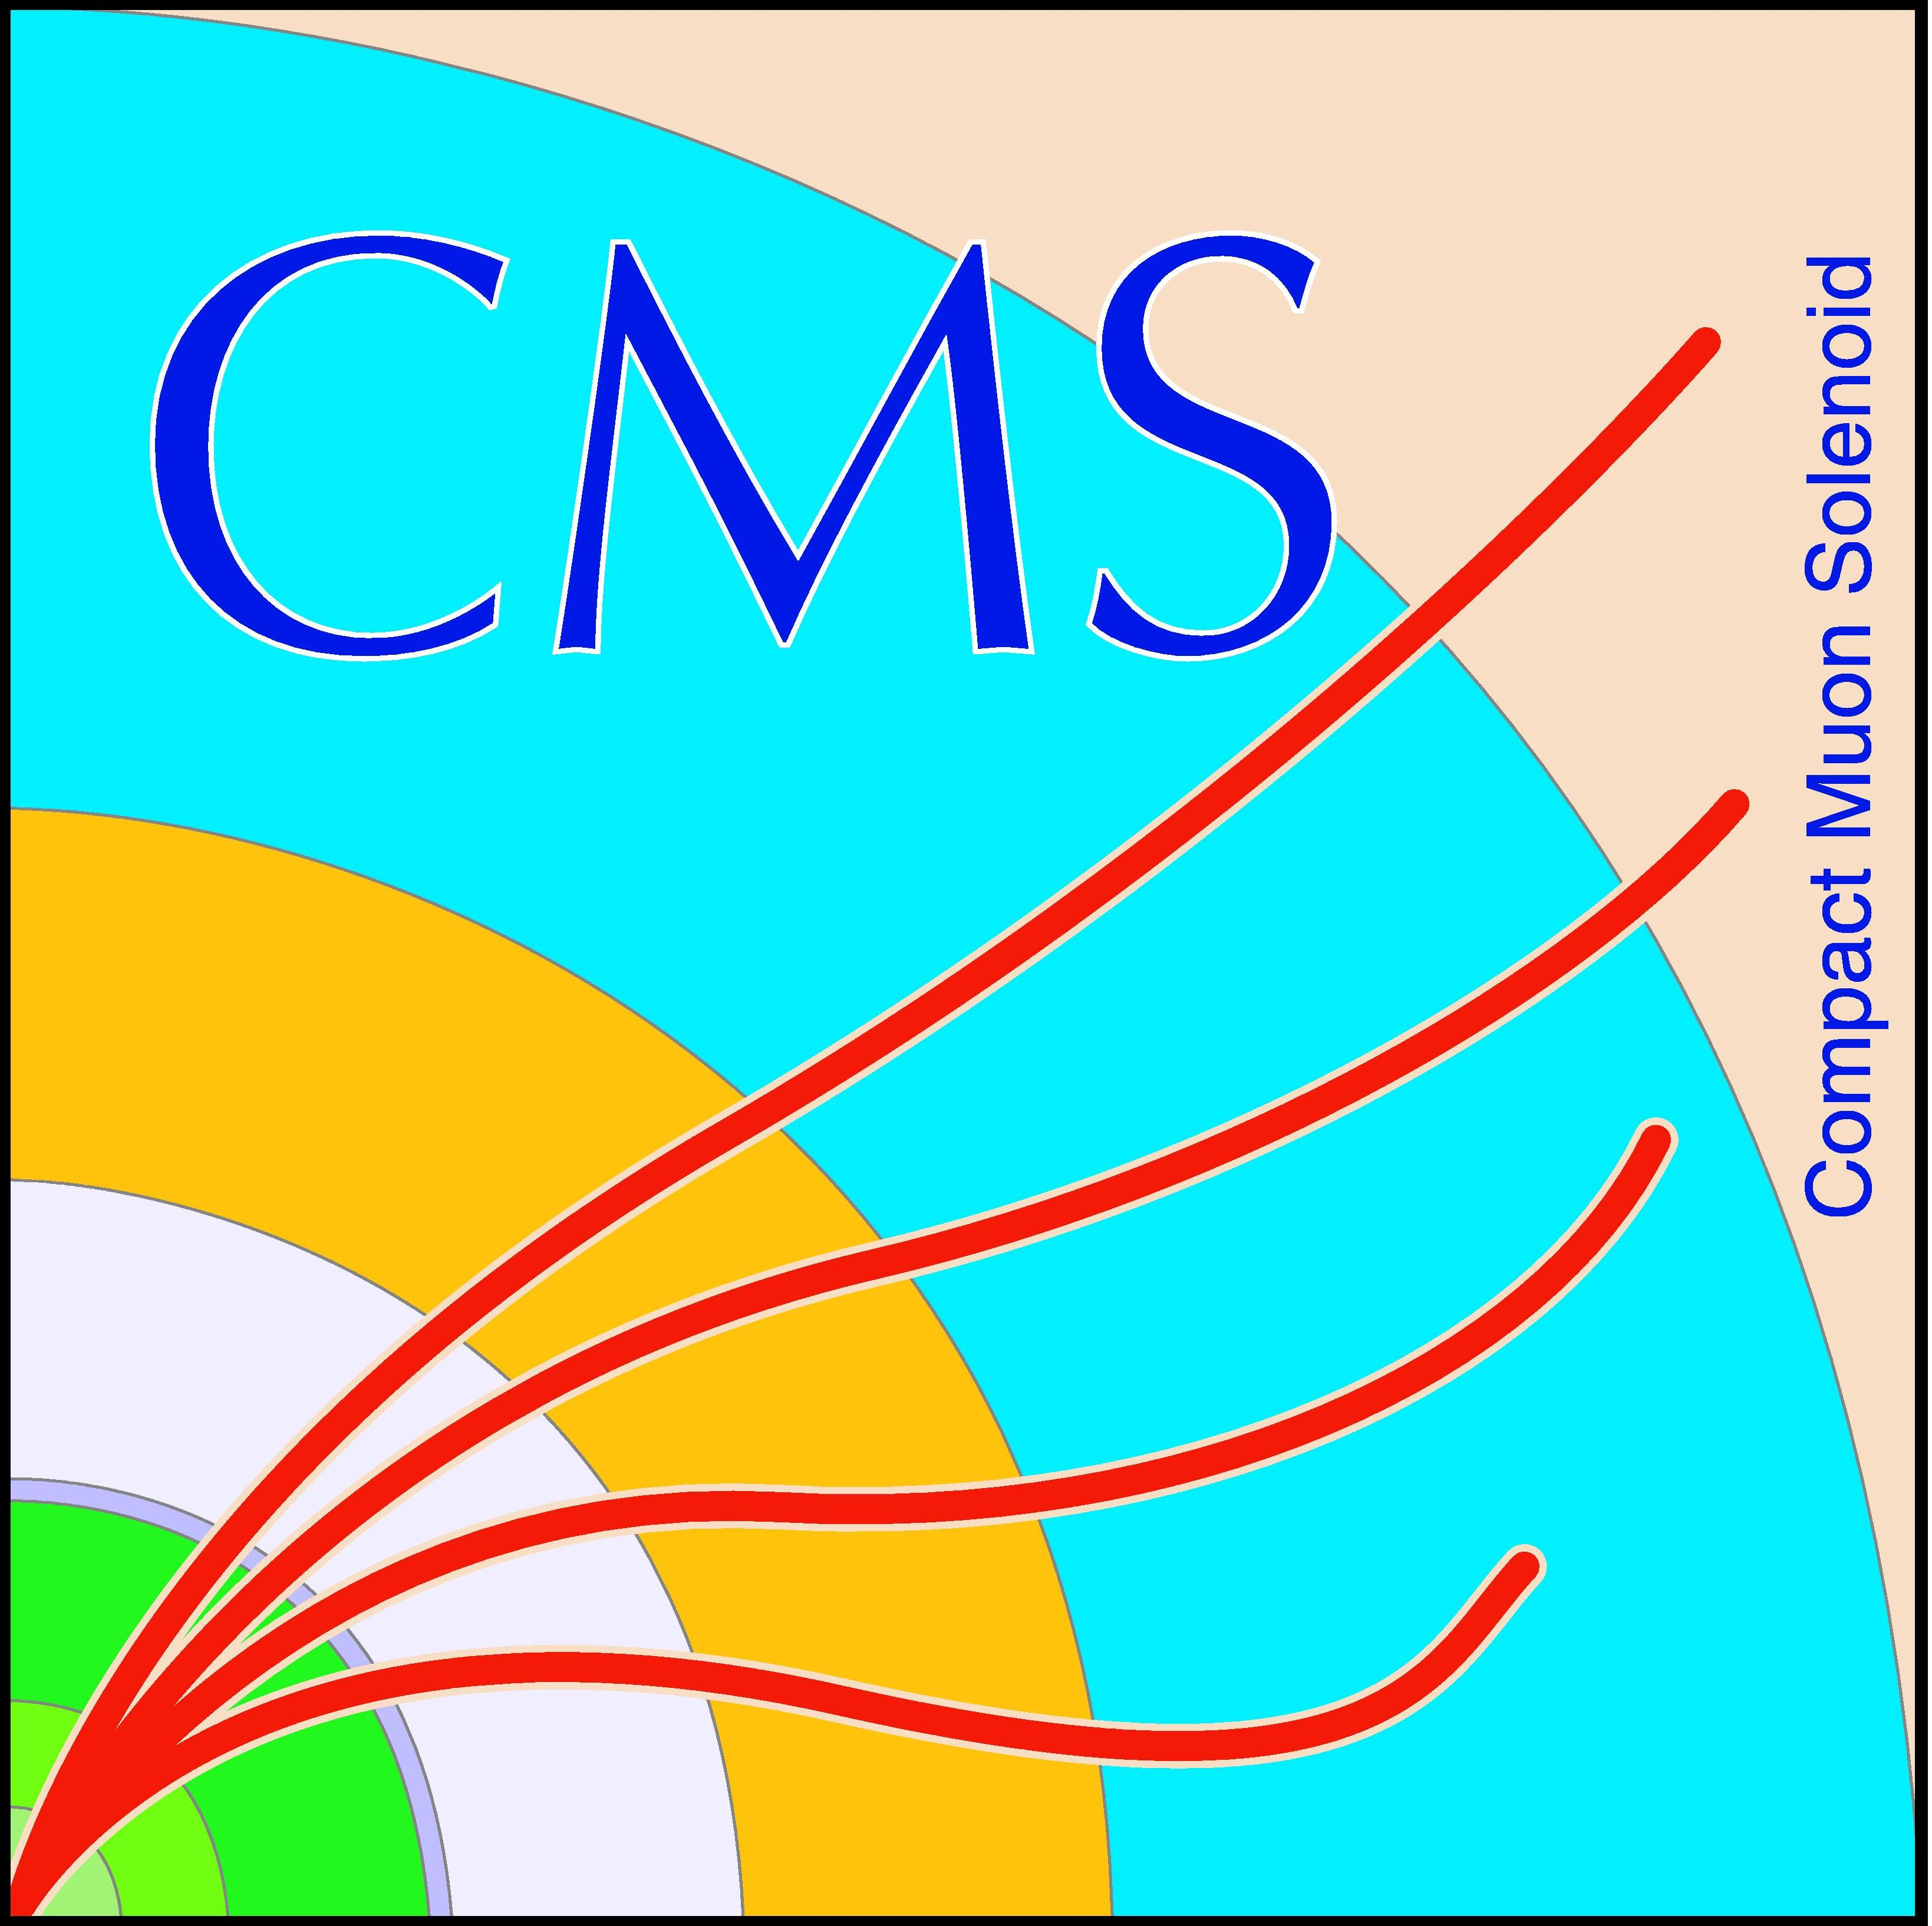
\includegraphics[height=1.5cm]{CMSlogo.jpeg}
  \end{center}
}

% pdflatex packages
\hypersetup{bookmarks=true}
\hypersetup{unicode=false}
\hypersetup{pdftitle={Lost-Lepton RA2/b}}
\hypersetup{pdfauthor={Arne-Rasmus~Dr\"ager}}


\begin{document}
% ==================================================
% --------------------------------------------------
\begin{frame}
  \titlepage
\end{frame}


% --------------------------------------------------
\section{Introduction}


\begin{frame}
  \frametitle{Lost-lepton Motivation}
  \begin{figure}
    \centering
    \begin{subfigure}[b]{0.3\textwidth}
      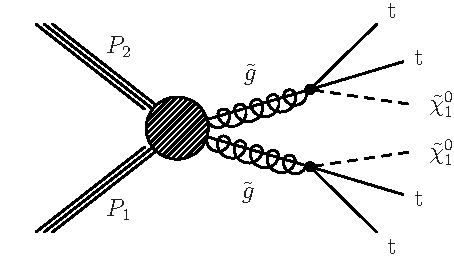
\includegraphics[width=\textwidth]{figures/jacks_Studies/T1tttt_feyn}
    \end{subfigure}%
    \begin{subfigure}[b]{0.3\textwidth}
      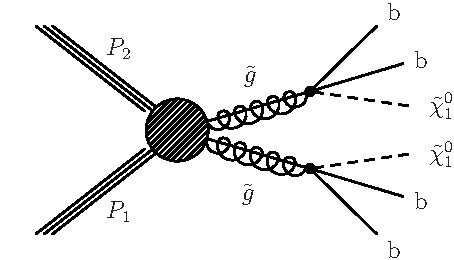
\includegraphics[width=\textwidth]{figures/jacks_Studies/T1bbbb_feyn}
    \end{subfigure}
    \begin{subfigure}[b]{0.3\textwidth}
      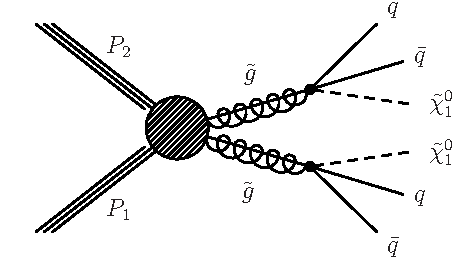
\includegraphics[width=\textwidth]{figures/jacks_Studies/T1qqqq}
    \end{subfigure}
    % \label{fig:models}
  \end{figure}
  \begin{itemize}
  \item RA2/b: inclusive hadronic analyses targeting gluino production (T1tttt, T1bbbb, T1qqqq)
  \item In most sensitive bins, main background is \ttbar events with lost-leptons
  \item T1tttt events have leptons $\sim 70 \%$ of the time
  \begin{itemize}
   \item Are rejected if any lepton passes isolation definition
   \item Enter control sample for background estimation methods
  \end{itemize}  
  \end{itemize}
\end{frame}

\begin{frame}
\frametitle{Baseline selection}
\normalsize
\begin{itemize}
 \item $\HT >500 \gev$
 \begin{itemize}
       \item Jets: $\pt>30\gev$, $|\eta|<2.5$
      \end{itemize}
 \item $\MHT >200 \gev$
  \begin{itemize}
       \item Jets: $\pt>30\gev$, $|\eta|<5.0$
      \end{itemize}
 \item $\NJets\ge 4$, \HT jets
 \item $\BTags$= {$0,1,2,\geq3$} CSVM ($>0.814$), $\pt>30\gev$
 \item $\deltaphi_{1,2,3}>0.5,0.5,0.3$
\item Veto Muons: \href{https://twiki.cern.ch/twiki/bin/view/CMSPublic/SWGuideMuonId\#Tight\_Muon}{2012 ``tight'' ID}: $p_T > 10$ GeV, $I_{rel}\; (\Delta R<0.4) < 0.2$    
    \item Veto Electrons: \href{https://twiki.cern.ch/twiki/bin/viewauth/CMS/CutBasedElectronIdentificationRun2\#CSA14\_selection\_conditions\_25ns}{Phys14 POG ID}:  $p_T > 10$ GeV, $I_{rel}\;
      (\Delta R<0.3) < 0.33 / 0.38$
      \item Under study:
      \begin{itemize}


    \item Taus: \href{https://indico.cern.ch/event/359233/contribution/4/material/slides/0.pdf}{Phys14 POG ID}: $p_T > 10$ GeV, $|\eta| < 2.3$,
      chargedIsoPtSum $(\Delta R<0.5)$ < 1.0 GeV (no neutral isolation yet)
    \item Isolated tracks: $p_T > 15$ GeV, $I_{rel}\;(\Delta R<0.3) < 0.1$ -- just charged candidates
      \end{itemize}
\end{itemize}
% \begin{block}{}
% \centering
% \Large
% \end{block}
\end{frame}

\section{Classical Lost-Lepton Method}
\begin{frame}
  \begin{center}
    {\Large
     Classical Lost-Lepton Prediction Method \\(Arne-Rasmus Draeger)}
  \end{center}
\end{frame}
\subsection{Basic concept}
\begin{frame}
  \frametitle{Mainly \ttbar and \wpj events where prompt electrons or muons are lost}
   \begin{figure}
 \centering
  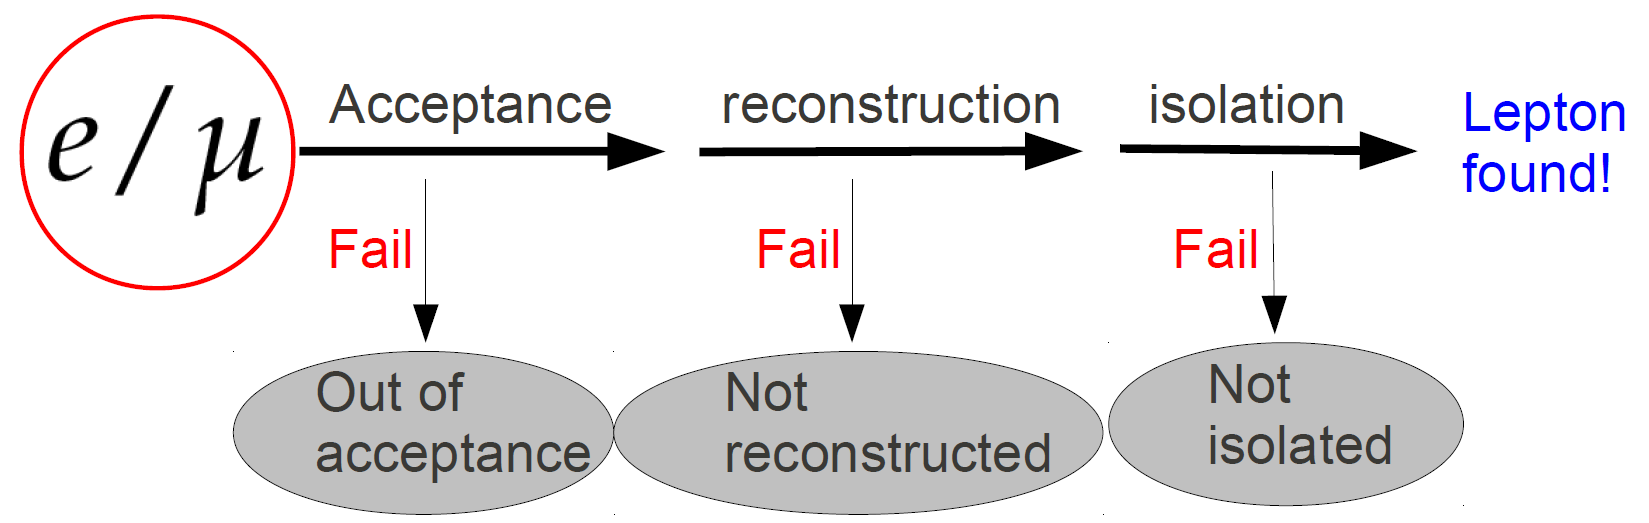
\includegraphics[width = 0.65\textwidth]{figures/lepton_veto_sketch.png}
%  \caption{Awesome figure}
 \end{figure}
      \begin{itemize}
      \item Select a control sample (CS) of exactly one well isolated \\electron, $\mu$ within the acceptance
        \begin{itemize}
        \item Weight each CS event according to efficiencies for each identification step
        \item Predict expected di-leptonic \ttbar contribution to lost-lepton background independently using the same single $e,\mu$ control sample (about 1\%)
        \item Combine independent prediction from single electron and $\mu$ for final prediction of lost-leptons
        \end{itemize}
      \end{itemize}
\end{frame}


\begin{frame}
\begin{itemize}
 \item Signal and other SM processes can contribute to e/$\mu$ control sample
 \item Suppress contamination by requiring trans. mass $\mt < 100 \gev$ \\
\end{itemize}
\vspace{0.5cm}
\hspace{0.5cm}$m_{T} = \sqrt{2 \cdot p_{T}(\mu/e)\cdot \met (1 - \cos(\Delta \Phi))}$

  \begin{columns}
    \begin{column}{0.5\textwidth}

      \begin{itemize}
      \item Removes about 10\% of e/$\mu$ CS due to:
        \begin{itemize}
        \item di-leptonic \ttbar decays
        \item Mismeasured jets
        \item Highly virtual W
        \end{itemize}
      \begin{centering}
      \end{centering}
      \item Correction for as a function of lepton $p_{T}$ \& activity around the lepton (motivation \& definition on the next slides)
      \end{itemize}
      \vspace{0.3cm}
    \end{column}
    \begin{column}{0.5\textwidth}
      \centering
    %  \begin{overpic}[width=0.8\textwidth]{figures/lost-lepton/ControlSample__MTW__MCPrMTWDiLepTTbar+MCPrMTWDiLepW__mu_control_sample.pdf}
%        \begin{overpic}[width=0.95\textwidth]{figures/deltaphicut/control-sample/ControlSample_Combined_searchbins__MTW__MCEx_vs_MuPrMTWDiLep+ElecPrMTWDiLep__Baseline.pdf}
\begin{overpic}[width=0.95\textwidth]{figures/deltaphicut/control-sample/mtw.png}
       \put(53.93,80){\color{black}\line(0,-1){67}}
    %\put(90,90){\rotatebox{-45}{\scriptsize \Large Arne}}
      \end{overpic}
    \end{column}
  \end{columns}

\end{frame}

%--------------------------------------------------------------------
\subsection{Efficiency Parametrization}
\begin{frame}
 \begin{columns}
  \begin{column}{0.4\textwidth}
  \normalsize
   \begin{itemize}
  \item In order to achieve good closure well parametrized and binned efficiency maps needed!
  \item Classical approach of lepton \pt (jet \pt) \& $\Delta R$ shows strong variation of efficiency and is strongly correlated with lepton isolation definition
  \item Severe problem when applying method in low statistical regions most sensitive search regions (hand full of events)
 \end{itemize}
  \end{column}
  \begin{column}{0.6\textwidth}
 
     \centering
     \small  Typical $\mu$ isolation efficiency
   \begin{overpic}[width=1.\textwidth]{figures/deltaphicut/efficiencies/8TeV/DataTAPmuIso.pdf}
     \end{overpic} \\
      
 Example: Region with 3 gen but only 1 CS event \\
   \begin{overpic} [width=0.45\textwidth]{figures/deltaRLowStat.pdf}
     \end{overpic}
     \begin{overpic} [width=0.45\textwidth]{figures/deltaRLowStatReco.pdf}
     \end{overpic} \\
    Here: Control sample lepton in high eff. region\\  $\rightarrow$ low weight $\rightarrow$ under-prediction
 
  \end{column}
 \end{columns}
%  \begin{itemize}
%   \item Low statistics in control sample combined with strong variation in efficiency leads to high uncertainties in most sensitive bins
%  \end{itemize}


\end{frame}
\begin{frame}
 \frametitle{Parametrization Problem \& 8 TeV solution}
  \begin{columns}
  \begin{column}{0.5\textwidth}
    \begin{itemize}
 \item Two main problems:
 \begin{itemize}
  \item Lepton isolation definition and $\Delta R<IsoCone$ combined with relative \pt are strongly correlated
  \item Steep drop in efficiency approaching IsoCone combined with low statistics of control sample in most sensitive search regions leads to high uncertainties
 \end{itemize}
 \end{itemize}
 \end{column}
 \begin{column}{0.5\textwidth}
  \begin{overpic}[width=1.\textwidth]{figures/deltaphicut/efficiencies/8TeV/DataTAPmuIso.pdf}
     \end{overpic} \\
 \end{column}

  \end{columns}

\begin{itemize}

\item In 8TeV RA2 used efficiencies binned in search variables following closely search region definition
  \begin{itemize}
  \item Good closure
   \item Relatively high statistical uncertainties on efficiency maps
   \item Could not be obtained from data only indirect validation via Tag \& Probe method
  \end{itemize}
  \end{itemize}
 

\end{frame}

\begin{frame}
 \frametitle{13 TeV Attempt (unoptimized)}
 \begin{itemize}
  \item New Ansatz: Lepton \pt together with activity ($A$) around the lepton in a larger fixed cone size (replace $\Delta R$)
 \begin{itemize}
  \item Not orthogonal but also not fully correlated to isolation definition $\rightarrow$ subset of energy in cone around lepton
 \item Capture event kinematics in a more broader framer 'averaging' over range of strong drop in $\Delta R$
 \end{itemize}
   \item Can in principle be obtained from data. % Capability of capturing kinematic differences between \Zmumu and \wpj, \ttbar need to be evaluated
   \item Integrate over some event information but gain more resistance against low statistics region fluctuations
  \item Muon activity:
  \begin{itemize}
   \item $A = \sum_{Jet}^{\Delta R<1.0} \pt(Jet) * (ChargedEMFraction + ChargedHadFraction) $
  \end{itemize}
    \item Electron activity:
  \begin{itemize}
   \item $A = \sum_{Jet}^{\Delta R<1.0} \pt(Jet) * (ChargedHadFraction) $
  \end{itemize}
 \end{itemize}

\end{frame}


% \begin{frame}
%  \frametitle{Solving parametrization problem (first attempt)}
%  \begin{itemize}
%   \item In 8TeV RA2 used efficiencies binned in search variables following closely search region definition
%   \begin{itemize}
%    \item Good closure
%    \item Relatively high statistical uncertainties on efficiency maps
%    \item Could not be obtained from data only indirect validation via Tag \& Probe method
%   \end{itemize}
%   \item Ansatz: Lepton \pt together with activity ($A$) around the lepton in a larger fixed cone size (replace $\Delta R$)
%   \begin{itemize}
%    \item 'Average' over $\Delta R$ capture event activity in a more broader picture. More activity in event more likely to lose lepton
%    \item Can in principle be obtained from data. % Capability of capturing kinematic differences between \Zmumu and \wpj, \ttbar need to be evaluated
%    \item Integrate over some event information but gain more resistance against low statistics region fluctuations
%   \end{itemize}
%    \item Muon activity:
%   \begin{itemize}
%    \item $A = \sum_{Jet}^{\Delta R<1.0} \pt(Jet) * (ChargedEMFraction + ChargedHadFraction) $
%   \end{itemize}
%     \item Electron activity:
%   \begin{itemize}
%    \item $A = \sum_{Jet}^{\Delta R<1.0} \pt(Jet) * (ChargedHadFraction) $
%   \end{itemize}
%   \end{itemize}
%
% %  \begin{block}{}
% %  \centering
% %  \Large First tests using this new variable for the reconstruction and isolation efficiencies
% %  \end{block}
% \end{frame}

%--------------------------------------------------------------------

\subsection{Closure Test}
\begin{frame}


\begin{itemize}
\item Closure test combining single $\mu$ \& $e$ control sample prediction
\end{itemize}
  \begin{columns}
    \begin{column}{0.5\textwidth}
     \centering
      \begin{overpic}[width=0.57\textwidth]{figures/deltaphicut/Closure_New_Parametrization/Closure_Combined__HT__MCEx_vs_MuPrMTWDiLep+ElecPrMTWDiLep__Baseline.pdf}
     \end{overpic}
           \begin{overpic}[width=0.57\textwidth]{figures/deltaphicut/Closure_New_Parametrization/Closure_Combined__NJets__MCEx_vs_MuPrMTWDiLep+ElecPrMTWDiLep__Baseline.pdf}
     \end{overpic}
    \end{column}
    \begin{column}{0.5\textwidth}
      \centering
            \begin{overpic}[width=0.57\textwidth]{figures/deltaphicut/Closure_New_Parametrization/Closure_Combined__MHT__MCEx_vs_MuPrMTWDiLep+ElecPrMTWDiLep__Baseline.pdf}
     %     \put(90,90){\rotatebox{-45}{\scriptsize \Large Arne}}
     \end{overpic}
     \begin{overpic}[width=0.57\textwidth]{figures/deltaphicut/Closure_New_Parametrization/Closure_Combined__BTags__MCEx_vs_MuPrMTWDiLep+ElecPrMTWDiLep__Baseline.pdf}
%       \begin{overpic}[width=0.57\textwidth]{figures/lost-lepton/Closure__NVtx__MCPrMTWDiLep_vs_MCEx__csa_Baseline.pdf}
      \end{overpic}
    \end{column}
  \end{columns}
  \begin{itemize}
  \item $\HT > 500 \gev$ , $\MHT>200 \gev$, $\NJets\ge 3$ , $\Delta\Phi_{1,2,3}>$0.5, 0.5, 0.3
   \item Reasonable closure (exp $3862.1 \pm 17.9$, pred $3742.9 \pm 27.4$)
  \end{itemize}


 
\end{frame}
  \begin{frame}
  \begin{center}
    {
     \large Extension of Classical Lost-Lepton Method:\\ \Large Extrapolation from mdium to high \MHT regions \\(Owen Long)}
  \end{center}
\end{frame}
\section{Extrapolation Method}
\begin{frame}
 \begin{itemize}
  \item Idea:
  \begin{itemize}
  \item Lost-lepton method limited by single lepton control sample statistics in some high \MHT search regions
   \item Reduce statistical uncertainties in high \MHT regions by extrapolating from medium to high \MHT regions using W decay helicity distributions (well known physics $\rightarrow$ MC reliable).
  \end{itemize}

 \end{itemize}
 \begin{center}
 


\begin{overpic}[width=0.85\textwidth]{figures/LostLeptonExtraPolationScatch.png}
%       \begin{overpic}[width=0.57\textwidth]{figures/lost-lepton/Closure__NVtx__MCPrMTWDiLep_vs_MCEx__csa_Baseline.pdf}
      \end{overpic}
       \end{center}
       \begin{itemize}
 \item Concept:
 \begin{itemize}
  \item Use single lepton data control sample to measure $\pt(W)$ spectrum
  \item Use cos($\Delta \Theta_{T}$) distribution from MC to predict lost-lepton \MHT spectrum
 \end{itemize}

\end{itemize}
\end{frame}
\begin{frame}
 \frametitle{Status of extrapolation technique}
 \begin{columns}
  \begin{column}{0.6\textwidth}
  \begin{itemize}
   \item Use classic lost-lepton method to estimate background at medium \MHT [200,500] and a \MHT ratio as a function of cos($\Delta \Theta_{T}$) to extrapolate to high \MHT    
   \item First try shows good closure in the relavant high \MHT search regions
   \item Increase in control sample statistics up to a factor of 4 to 7 in respect to single lepton estimation method
   \item \wpj and di-leptonic \ttbar events need to be accounted for as well
   \item Uncertainties need to evaluated and compared to classical method to judge on the gain
  \end{itemize}

   
  \end{column}
  \begin{column}{0.4\textwidth}
   \begin{overpic}[width=0.90\textwidth]{figures/LostLeptonHelicityPlot.png}
      \end{overpic}\\
         \begin{overpic}[width=0.90\textwidth]{figures/LostLeptonExtrapolationClosure.png}
      \end{overpic}\\
  \end{column}


 \end{columns}
  \centering
\small More information: Presentation \href{https://indico.cern.ch/event/334951/contribution/0/material/slides/0.pdf}{1}, \href{https://indico.cern.ch/event/360073/contribution/0/material/slides/0.pdf}{2}
\end{frame}




\subsection{Conclusion}
\begin{frame}
 \frametitle{Lost-Lepton Methods Conclusion}
 \begin{itemize}
 \item Classic lost-lepton method:
 \begin{itemize}
  \item Extension of lost-lepton method from using single $e$ \& $\mu$ control sample with an important improvement of statistical uncertainty $\sqrt{2}$ (largest uncertainty in many very sensitive bins at 8 TeV data) works
  \item Activity variable shows good performance as lepton efficiency parametrization
  \item Further studies are ongoing exploring various variables for binning the efficiencies
 \end{itemize}
 \item Lost-lepton extrapolation method:
 \begin{itemize}
  \item Attempt of further decreasing of statistical uncertainty in some of the most sensitive bins by extrapolating from medium to high \MHT region
  \item First attempt shows good closure
  \item Gain in respect to classical lost-lepton method statistics by a factor of 4-7 for relevant bins
  \item Uncertainties need to be evaluated and compared with classical lost-lepton approach to judge on expected improvement
 \end{itemize}

 \end{itemize}

\end{frame}


\section{Optimization Studies}
  \begin{frame}
  \begin{center}
    {
     \large Optimization Studies on \ttbar \& \wpj background event rejection \\(Jack Bradmiller-Feld)}
  \end{center}
\end{frame}

\subsection{Optimization}
\begin{frame}
  \frametitle{Lepton composition at truth level}
  \begin{columns}[c] % the "c" option specifies center vertical alignment
    \column{.5\textwidth} % column designated by a command
    After baseline selection, more than $\sim60\%$ of $t\bar{t}$
    events contain taus
    \begin{figure}
      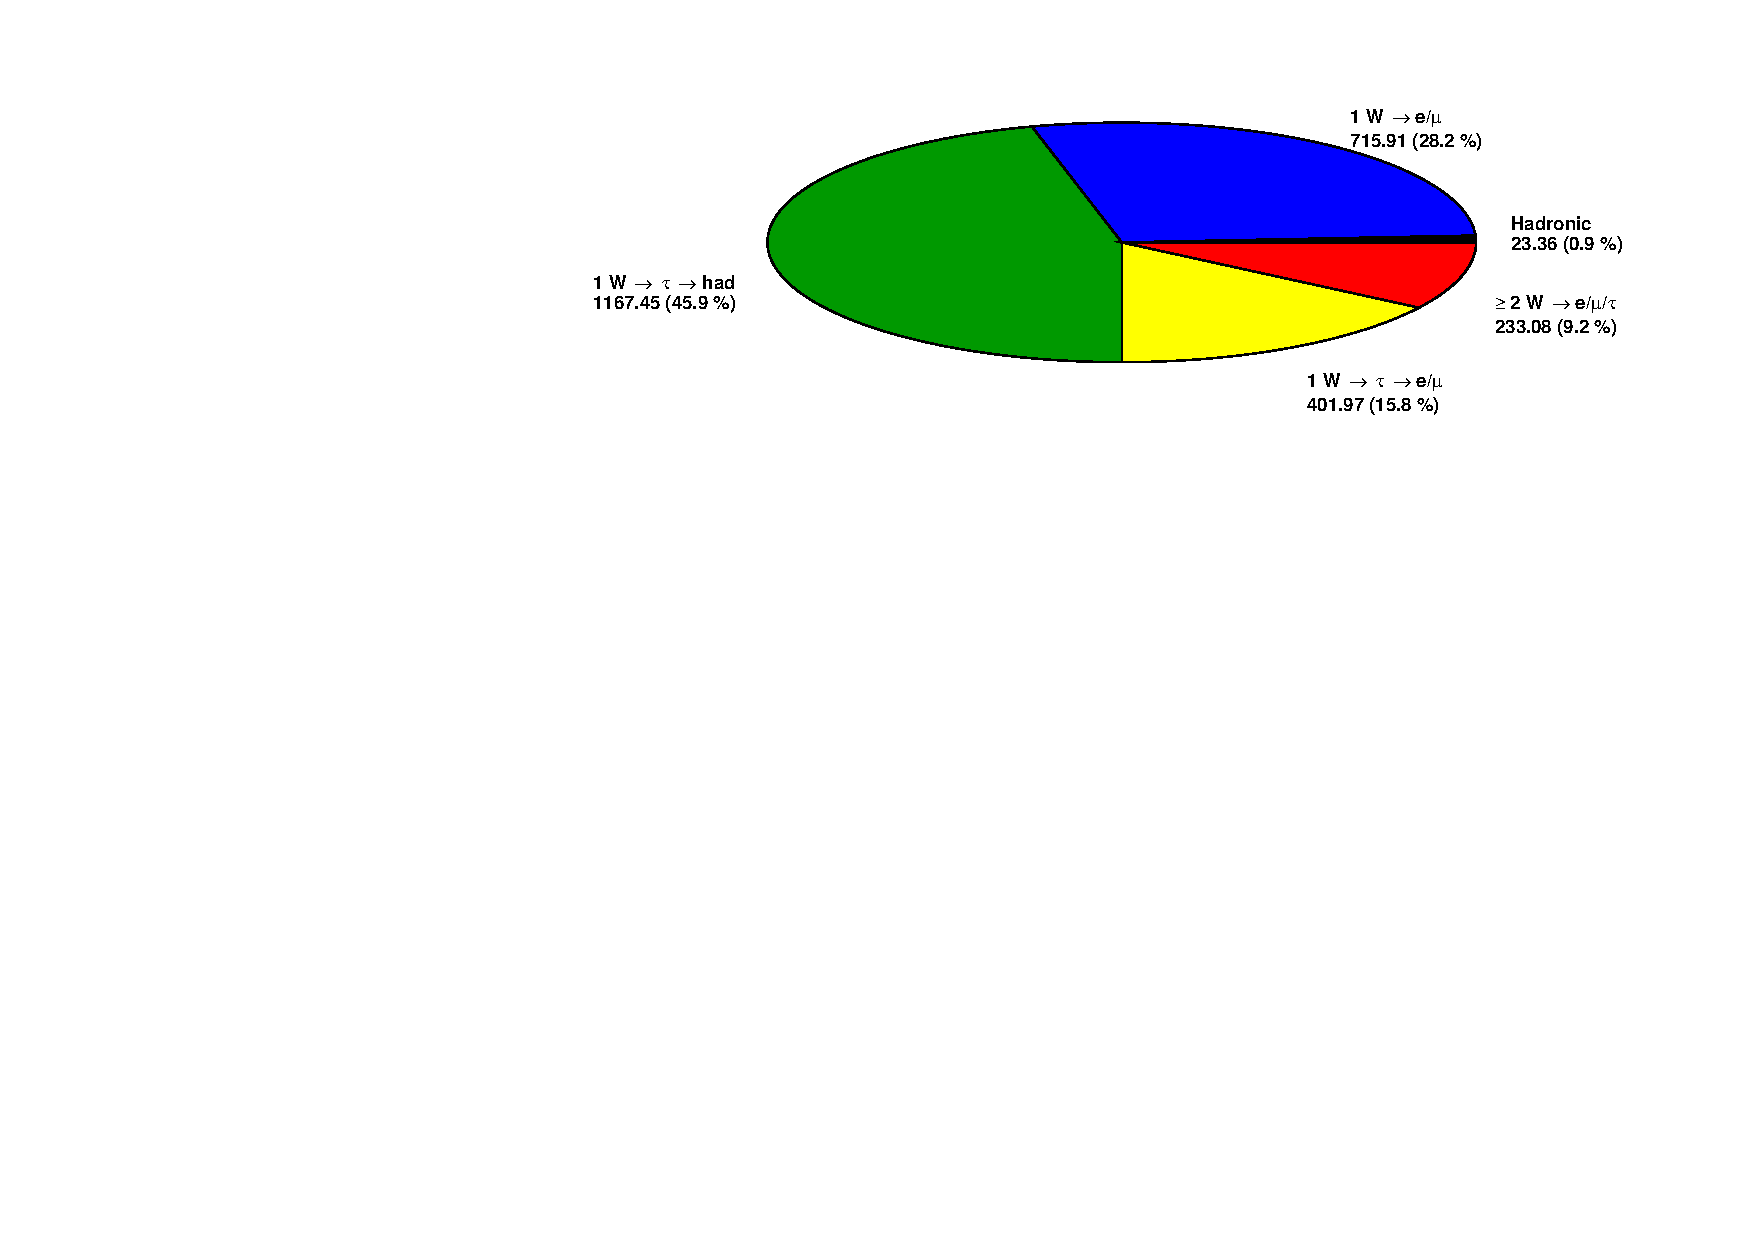
\includegraphics[width=1.2\textwidth]{figures/jacks_Studies/lepton_piechart_ttbar_baseline_117}
    \end{figure}
    \column{.5\textwidth}
    About $\sim40\%$ of T1tttt events contain $e/\mu$
    \begin{figure}
      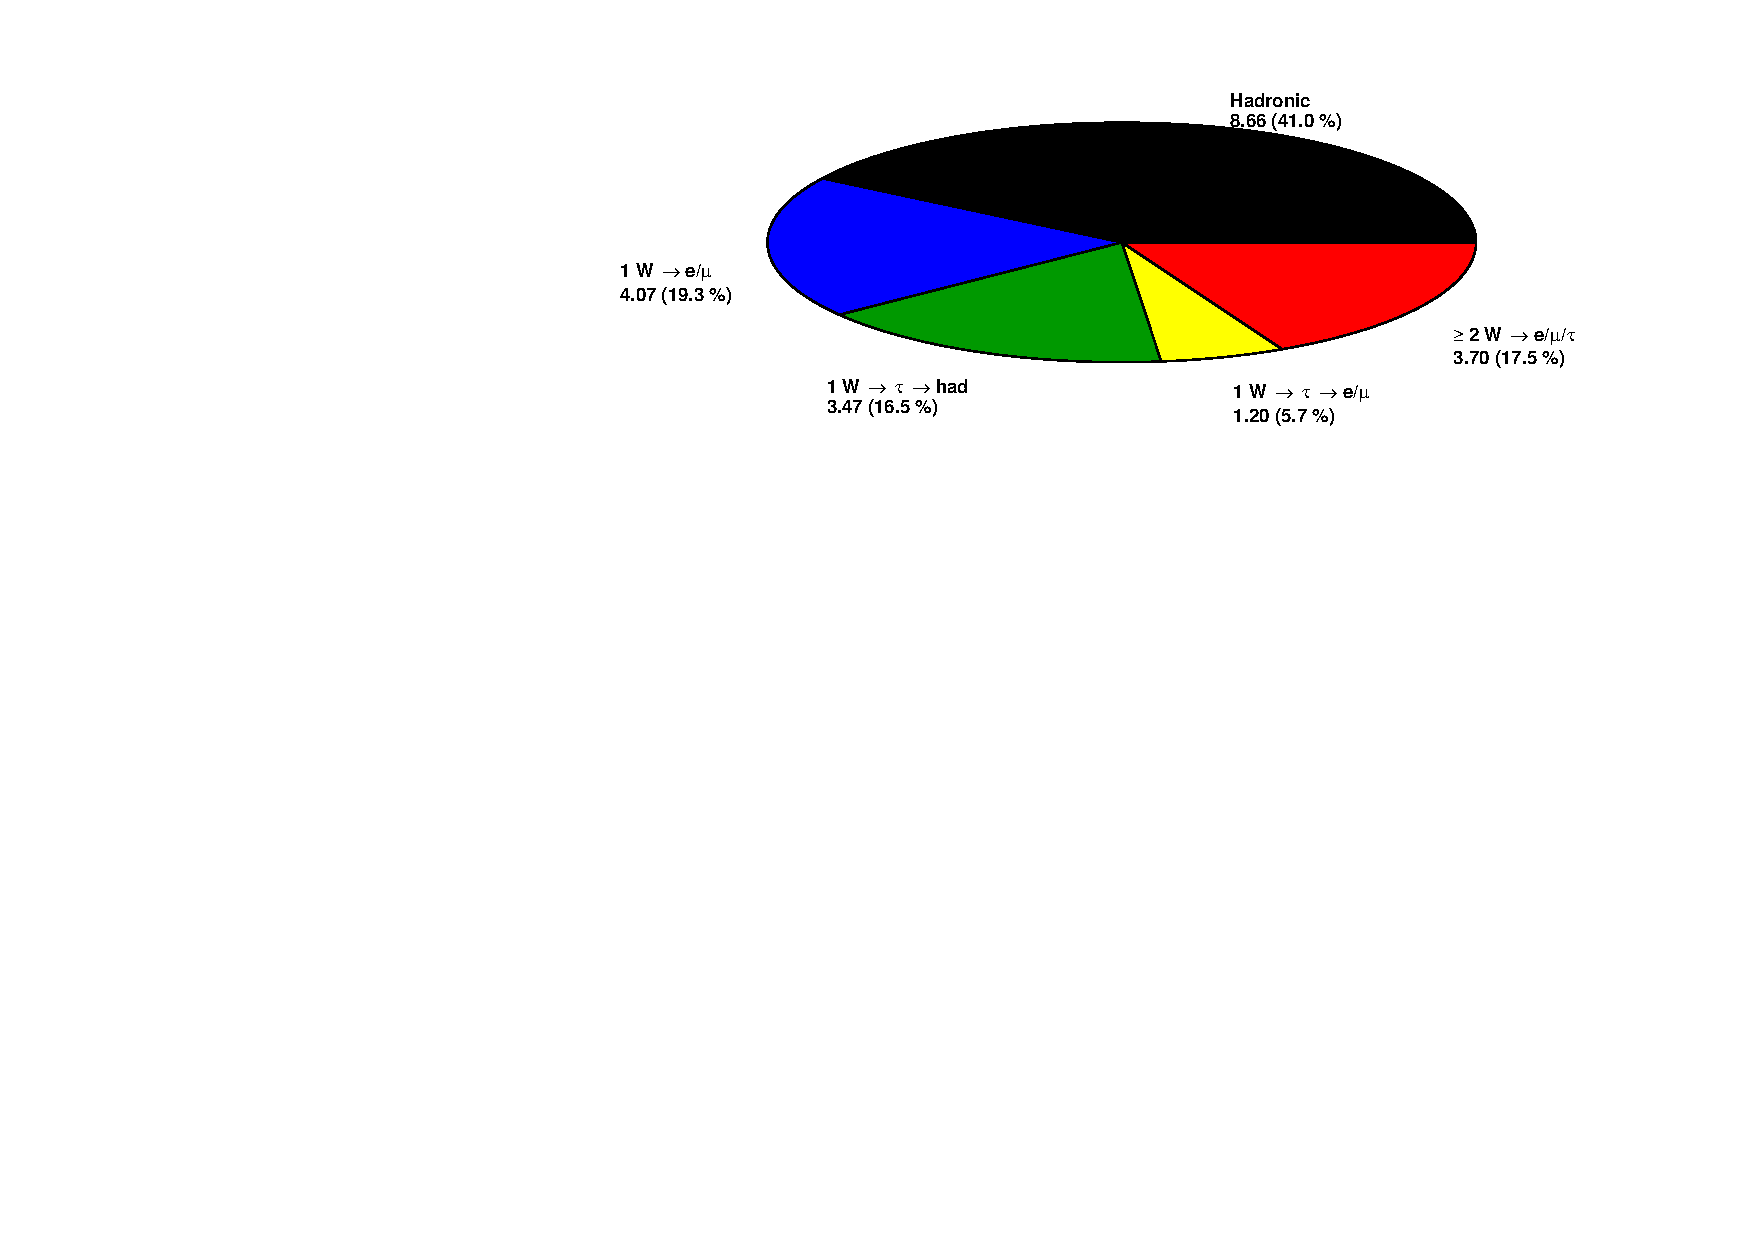
\includegraphics[width=1.2\textwidth]{figures/jacks_Studies/lepton_piechart_t1tttt_1500_100_baseline_117}
    \end{figure}
  \end{columns}
  \begin{itemize}
  \item Try to reject more $t\bar{t}$ \wpj BG with
    \begin{itemize}
    \item Single-prong tau veto
    \item Isolated track veto
    \end{itemize}
  \item For each object, compute and cut at $m_T(W) <100 \gev$
  \begin{itemize}
   \item Good efficiency for SM events
   \item Strong rejection of expected signal events
  \end{itemize}

  \item Can we save signal by not vetoing events with taus/tracks
    with $m_T>100$ GeV?
  \end{itemize}
\end{frame}

\begin{frame}
  \frametitle{Using $m_T(W)$ to save signal}
  \begin{itemize}
  \item We know that events with 1 true lepton and one source of MET
    ($W\rightarrow l\nu$ decay) are efficiently selected with $m_T<100$ GeV (90\%)
  \item If we only reject events with single isolated e or $\mu$ (taus or
    tracks) satisfying the above (or $m_T<100$), can we save any signal?
  \item This idea was also suggested by \href{https://indico.cern.ch/event/339666/session/2/contribution/50/material/slides/0.pdf}{Jason Gran / MT2 group}
  \end{itemize}
  \begin{figure}[h]
    \centering
    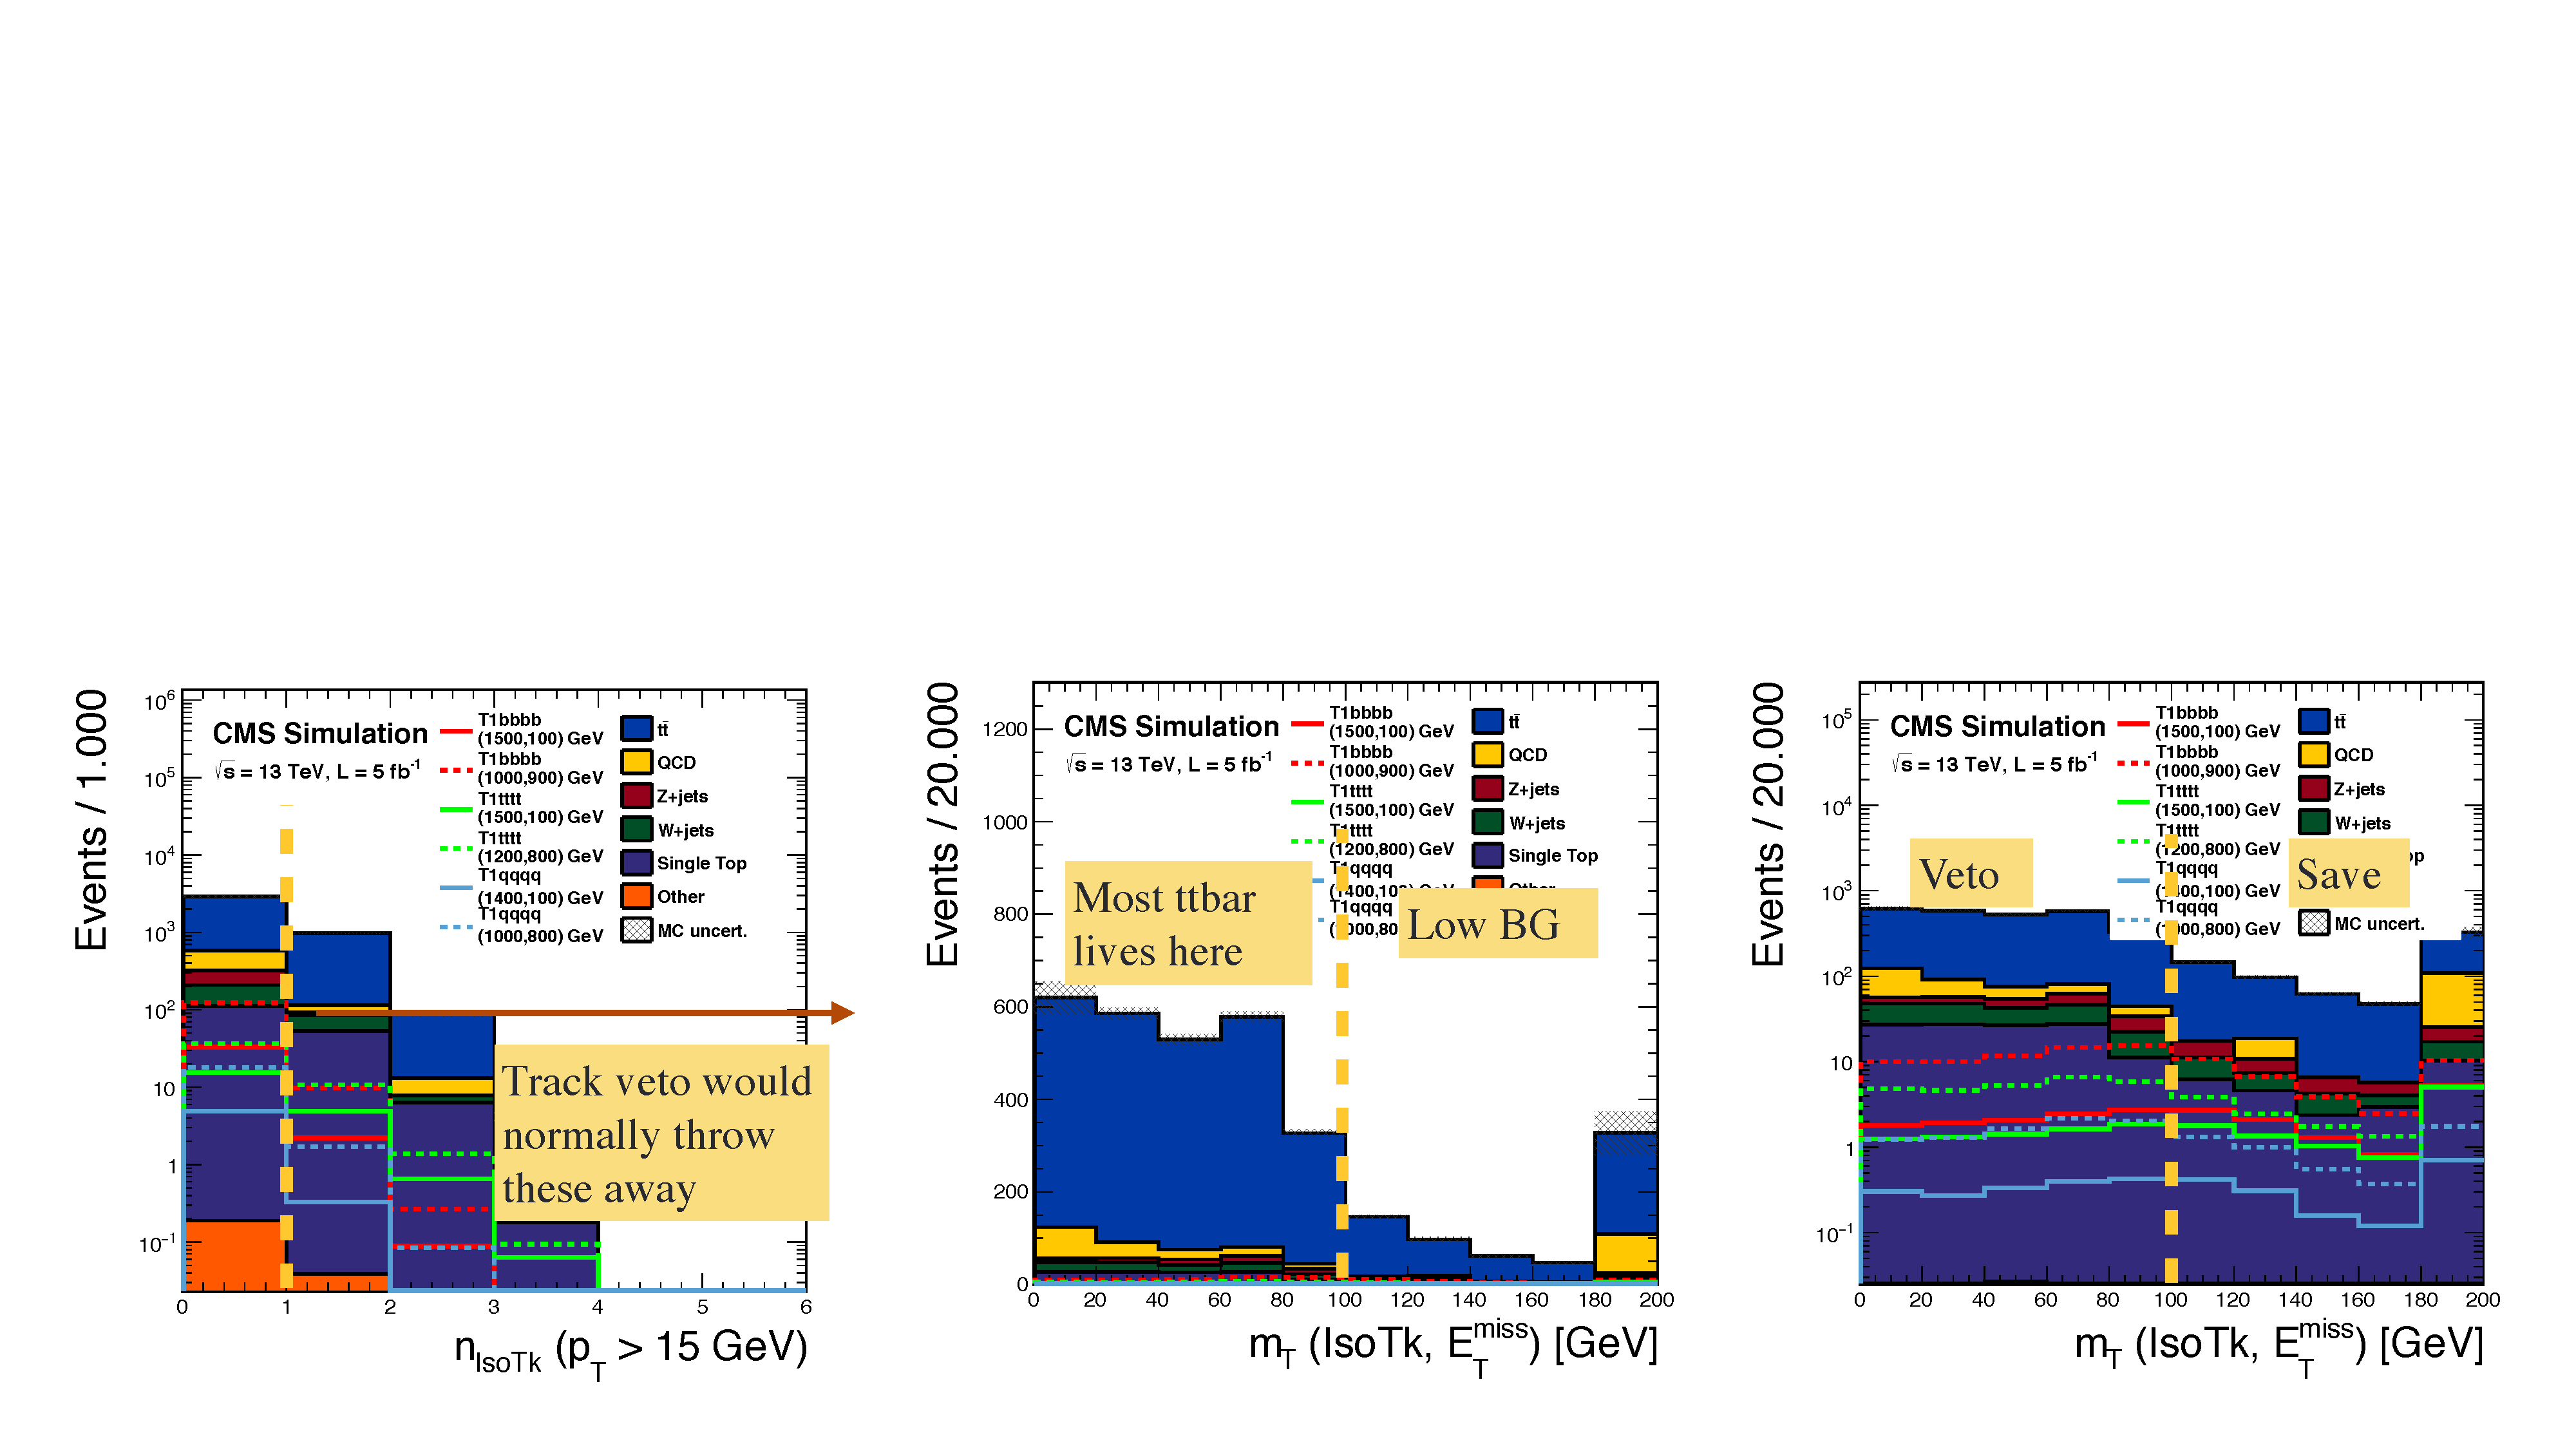
\includegraphics[width=\textwidth]{figures/jacks_Studies/mTIsoTracks}
  \end{figure}
\end{frame}

\begin{frame}
  \frametitle{Lepton event rejection cut flow $(5\mathrm{fb}^{-1})$}
  \begin{columns}[c] % the "c" option specifies center vertical alignment
    \column{.7\textwidth}
    \begin{figure}[h]
      \centering
      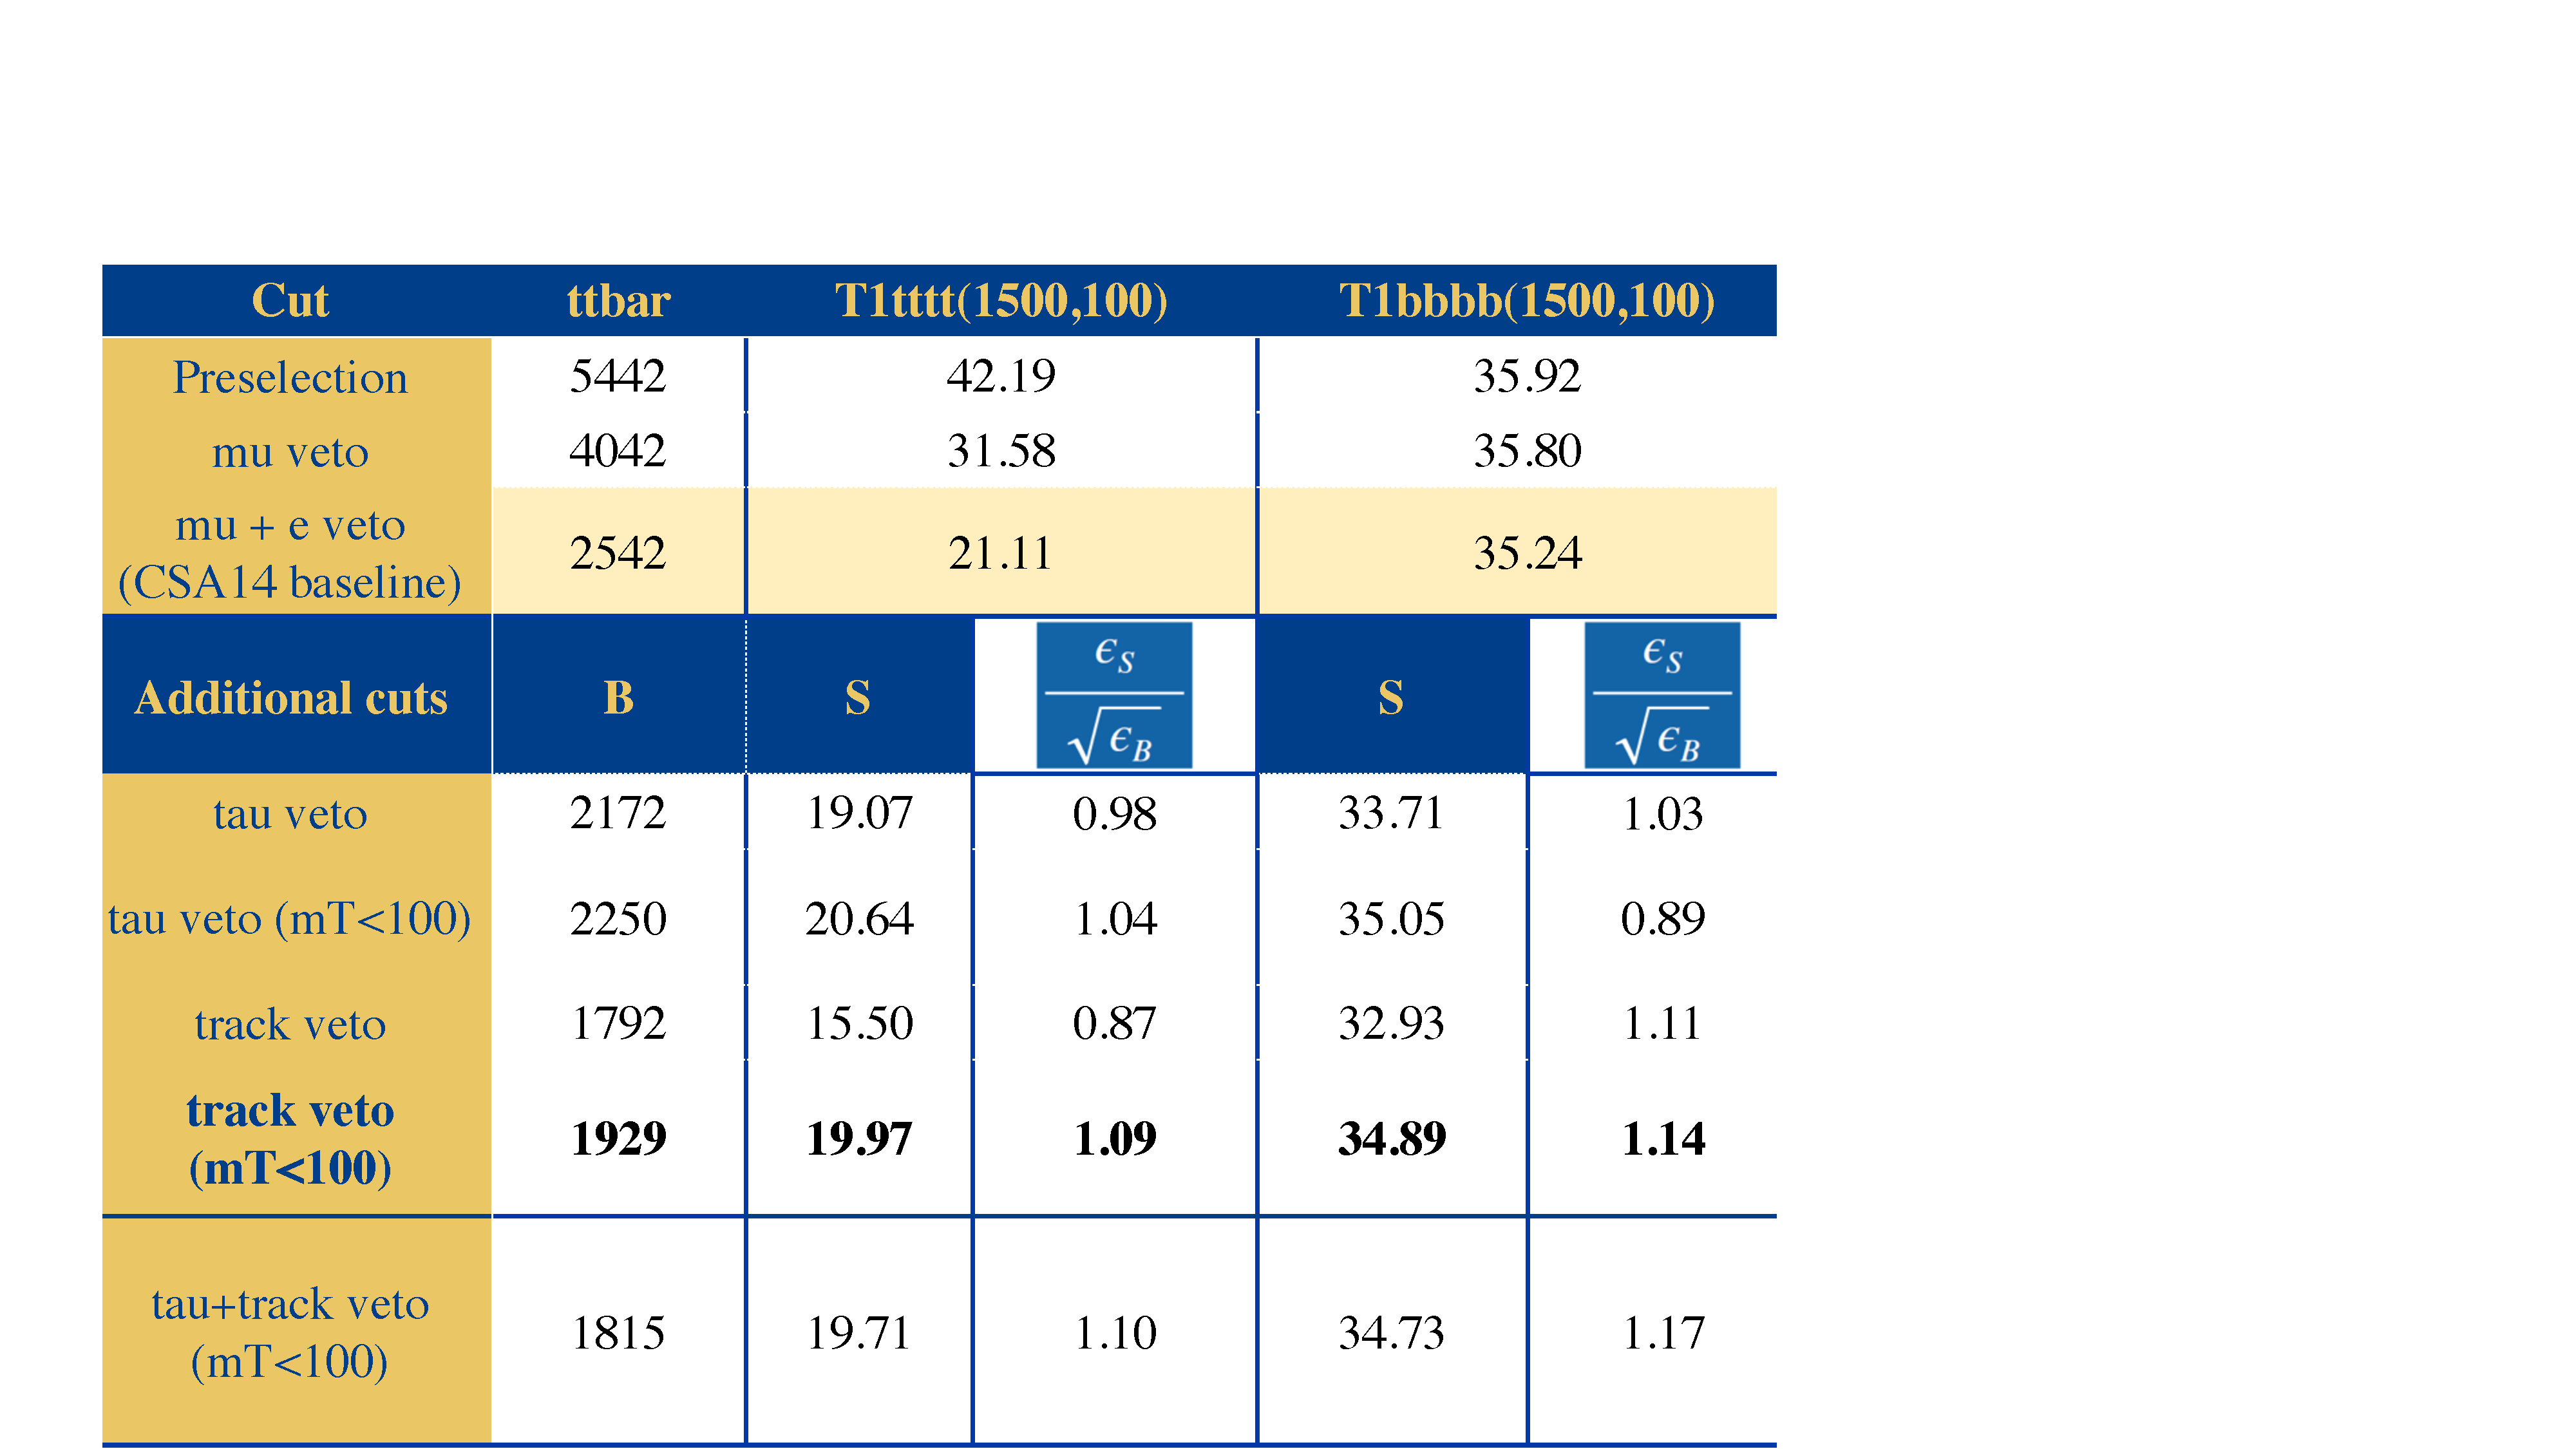
\includegraphics[width=\textwidth]{figures/jacks_Studies/cutflow_baseline}
    \end{figure}
    \column{.3\textwidth}
    \begin{itemize}
    \item Only rejecting events with $m_T(\tau,\;
      E_{T}^{\mathrm{miss}})$ or $m_T(tk,\; E_{T}^{\mathrm{miss}}) <
      100$ saves both T1bbbb and T1tttt
    \item Track veto seems most effective--for Phys14 AN, will only use
      this, skip $\tau$ veto
    \end{itemize}
  \end{columns}
  \vskip1cm
  \centering
\small More information: \href{https://indico.cern.ch/event/360072/contribution/0/material/slides/0.pdf}{Presentation}
\end{frame}


\subsection{Conclusion}
\begin{frame}
  \frametitle{Lepton \& Track Veto: Conclusions}
  \begin{itemize}
  \item Isolated track veto with $m_T<100$ restriction shows great
    improvement in sensitivity $(10-15\%)$ gain in
    $S/\sqrt{B}$
    \item Will be used for Phys14 on top of standard
    $e/\mu$ veto.
    \item Optimization of lepton \& isolated track definition
  \item Want to further reduce hadronic $\tau$ background:
    \begin{itemize}
    \item Looking into separate isolation recipes for hadronic tracks vs. $e/\mu$
      tracks
    \item Want to use neutral PFcands to calculate isolation as well, may
      help to characterize $\tau$ decays.
    \end{itemize}
  \item $\tau$ veto may also be useful at some point.
  \item Lost-lepton background estimation methods are being extended for isolated track veto
  \end{itemize}
\end{frame}










% --------------------------------------------------
% --------------------------------------------------
\section{MinDeltaPhiN}
\begin{frame}
  \begin{center}
    {\Large MinDeltaPhiN vs DeltaPhi123 cut}
  \end{center}
\end{frame}

\begin{frame}
\frametitle{Parametrization of Efficiencies}
  \begin{columns}
    \begin{column}{0.5\textwidth}
     \centering
     \deltaphi 
             \begin{itemize}


        \item Isolation
   \begin{itemize}
    \item Lep \pt Activity
   \end{itemize}
   \item Reconstruction
   \begin{itemize}
    \item Activity
   \end{itemize}
   \item Acceptance
   \begin{itemize}
    \item \BTags \NJets
   \end{itemize}
   \item Purity (only electron CS)
   \begin{itemize}
    \item \MHT \NJets
   \end{itemize}
      \item Di-lep contamination
   \begin{itemize}
    \item \NJets
   \end{itemize}
   \item Di-lep efficiency
   \begin{itemize}
    \item \NJets
   \end{itemize}
   \item \mt cut efficiency
   \begin{itemize}
    \item Activity
   \end{itemize}
     \end{itemize}
    \end{column}
    \begin{column}{0.5\textwidth}
      \centering
      \mindeltaphi
                   \begin{itemize}


        \item Isolation
   \begin{itemize}
    \item Lep \pt Activity
   \end{itemize}
   \item Reconstruction
   \begin{itemize}
    \item Activity
   \end{itemize}
   \item Acceptance
   \begin{itemize}
    \item\MHT \NJets
   \end{itemize}
   \item Purity (only electron CS)
   \begin{itemize}
    \item \MHT \NJets
   \end{itemize}
      \item Di-lep contamination
   \begin{itemize}
    \item \NJets
   \end{itemize}
   \item Di-lep efficiency
   \begin{itemize}
    \item \NJets
   \end{itemize}
   \item \mt cut efficiency
   \begin{itemize}
    \item Activity
   \end{itemize}
     \end{itemize}
    \end{column}
    \begin{column}{0.5\textwidth}

    \end{column}
  \end{columns}
\end{frame}

\subsection{Closure}
\begin{frame}
 \begin{center}
    {\Large Comparison \\ \deltaphi vs \mindeltaphi selection}
  \end{center}
\end{frame}

\begin{frame}
  \begin{columns}
    \begin{column}{0.5\textwidth}
     \centering
     \large \deltaphi cut \\
%       \begin{overpic}[width=0.70\textwidth]{figures/deltaphicut/Closure_Old_Parametrization/Closure__HT__MuPrMTWDiLep_vs_MCEx__Baseline.pdf}\put(100,60){\rotatebox{-90}{\scriptsize \deltaphi cut}}
%      \end{overpic}
      \begin{overpic}[width=0.70\textwidth]{figures/deltaphicut/Closure_New_Parametrization/Closure_Combined__HT__MCEx_vs_MuPrMTWDiLep+ElecPrMTWDiLep__Baseline.pdf} \end{overpic}
      \begin{overpic}[width=0.70\textwidth]{figures/deltaphicut/Closure_New_Parametrization/Closure_Combined__MHT__MCEx_vs_MuPrMTWDiLep+ElecPrMTWDiLep__Baseline.pdf} \end{overpic}

    \end{column}
    \begin{column}{0.5\textwidth}
      \centering
      \large \mindeltaphi cut \\
      \begin{overpic}[width=0.70\textwidth]{figures/mindeltaphicut/Closure/Closure_combined__HT__MCEx_vs_MuPrMTWDiLep+ElecPrMTWDiLep__Baseline.pdf} \end{overpic}
      \begin{overpic}[width=0.70\textwidth]{figures/mindeltaphicut/Closure/Closure_combined__MHT__MCEx_vs_MuPrMTWDiLep+ElecPrMTWDiLep__Baseline.pdf} \end{overpic}

    \end{column}
  \end{columns}
\end{frame}


\begin{frame}
  \begin{columns}
    \begin{column}{0.5\textwidth}
     \centering
     \large \deltaphi cut \\
%       \begin{overpic}[width=0.70\textwidth]{figures/deltaphicut/Closure_Old_Parametrization/Closure__HT__MuPrMTWDiLep_vs_MCEx__Baseline.pdf}\put(100,60){\rotatebox{-90}{\scriptsize \deltaphi cut}}
%      \end{overpic}
      \begin{overpic}[width=0.70\textwidth]{figures/deltaphicut/Closure_New_Parametrization/Closure_Combined__NJets__MCEx_vs_MuPrMTWDiLep+ElecPrMTWDiLep__Baseline.pdf} \end{overpic}
      \begin{overpic}[width=0.70\textwidth]{figures/deltaphicut/Closure_New_Parametrization/Closure_Combined__BTags__MCEx_vs_MuPrMTWDiLep+ElecPrMTWDiLep__Baseline.pdf} \end{overpic}

    \end{column}
    \begin{column}{0.5\textwidth}
      \centering
      \large \mindeltaphi cut \\
      \begin{overpic}[width=0.70\textwidth]{figures/mindeltaphicut/Closure/Closure_combined__NJets__MCEx_vs_MuPrMTWDiLep+ElecPrMTWDiLep__Baseline.pdf} \end{overpic}
      \begin{overpic}[width=0.70\textwidth]{figures/mindeltaphicut/Closure/Closure_combined__BTags__MCEx_vs_MuPrMTWDiLep+ElecPrMTWDiLep__Baseline.pdf} \end{overpic}

    \end{column}
  \end{columns}
\end{frame}

\subsection{Closure}
\begin{frame}
 \begin{center}
    {\Large Comparison \\ \deltaphi vs \mindeltaphi selection\\ Separate $\mu$ closure}
  \end{center}
\end{frame}

\begin{frame}
 \begin{center}
    {\Large $\mu$ iso closure}
  \end{center}
\end{frame}

\begin{frame}
  \begin{columns}
    \begin{column}{0.5\textwidth}
     \centering
     \large \deltaphi cut \\
%       \begin{overpic}[width=0.70\textwidth]{figures/deltaphicut/Closure_Old_Parametrization/Closure__HT__MuPrMTWDiLep_vs_MCEx__Baseline.pdf}\put(100,60){\rotatebox{-90}{\scriptsize \deltaphi cut}}
%      \end{overpic}
      \begin{overpic}[width=0.70\textwidth]{figures/deltaphicut/separate_closure/Mu_Closure_test__HT__MuExIso_vs_MuCSPrIso__Baseline.pdf} \end{overpic}
      \begin{overpic}[width=0.70\textwidth]{figures/deltaphicut/separate_closure/Mu_Closure_test__HT__MuExIso_vs_ElecCSPrIso__Baseline.pdf} \end{overpic}

    \end{column}
    \begin{column}{0.5\textwidth}
      \centering
      \large \mindeltaphi cut \\
      \begin{overpic}[width=0.70\textwidth]{figures/mindeltaphicut/separate_closure/Mu_Closure__HT__MuExIso_vs_MuCSPrIso__Baseline.pdf} \end{overpic}
      \begin{overpic}[width=0.70\textwidth]{figures/mindeltaphicut/separate_closure/Mu_Closure__HT__MuExIso_vs_ElecCSPrIso__Baseline.pdf} \end{overpic}

    \end{column}
  \end{columns}
\end{frame}


\begin{frame}
  \begin{columns}
    \begin{column}{0.5\textwidth}
     \centering
     \large \deltaphi cut \\
%       \begin{overpic}[width=0.70\textwidth]{figures/deltaphicut/Closure_Old_Parametrization/Closure__HT__MuPrMTWDiLep_vs_MCEx__Baseline.pdf}\put(100,60){\rotatebox{-90}{\scriptsize \deltaphi cut}}
%      \end{overpic}
      \begin{overpic}[width=0.70\textwidth]{figures/deltaphicut/separate_closure/Mu_Closure_test__MHT__MuExIso_vs_MuCSPrIso__Baseline.pdf} \end{overpic}
      \begin{overpic}[width=0.70\textwidth]{figures/deltaphicut/separate_closure/Mu_Closure_test__MHT__MuExIso_vs_ElecCSPrIso__Baseline.pdf} \end{overpic}

    \end{column}
    \begin{column}{0.5\textwidth}
      \centering
      \large \mindeltaphi cut \\
      \begin{overpic}[width=0.70\textwidth]{figures/mindeltaphicut/separate_closure/Mu_Closure__MHT__MuExIso_vs_MuCSPrIso__Baseline.pdf} \end{overpic}
      \begin{overpic}[width=0.70\textwidth]{figures/mindeltaphicut/separate_closure/Mu_Closure__MHT__MuExIso_vs_ElecCSPrIso__Baseline.pdf} \end{overpic}

    \end{column}
  \end{columns}
\end{frame}


\begin{frame}
  \begin{columns}
    \begin{column}{0.5\textwidth}
     \centering
     \large \deltaphi cut \\
%       \begin{overpic}[width=0.70\textwidth]{figures/deltaphicut/Closure_Old_Parametrization/Closure__HT__MuPrMTWDiLep_vs_MCEx__Baseline.pdf}\put(100,60){\rotatebox{-90}{\scriptsize \deltaphi cut}}
%      \end{overpic}
      \begin{overpic}[width=0.70\textwidth]{figures/deltaphicut/separate_closure/Mu_Closure_test__NJets__MuExIso_vs_MuCSPrIso__Baseline.pdf} \end{overpic}
      \begin{overpic}[width=0.70\textwidth]{figures/deltaphicut/separate_closure/Mu_Closure_test__NJets__MuExIso_vs_ElecCSPrIso__Baseline.pdf} \end{overpic}

    \end{column}
    \begin{column}{0.5\textwidth}
      \centering
      \large \mindeltaphi cut \\
      \begin{overpic}[width=0.70\textwidth]{figures/mindeltaphicut/separate_closure/Mu_Closure__NJets__MuExIso_vs_MuCSPrIso__Baseline.pdf} \end{overpic}
      \begin{overpic}[width=0.70\textwidth]{figures/mindeltaphicut/separate_closure/Mu_Closure__NJets__MuExIso_vs_ElecCSPrIso__Baseline.pdf} \end{overpic}

    \end{column}
  \end{columns}
\end{frame}

\begin{frame}
  \begin{columns}
    \begin{column}{0.5\textwidth}
     \centering
     \large \deltaphi cut \\
%       \begin{overpic}[width=0.70\textwidth]{figures/deltaphicut/Closure_Old_Parametrization/Closure__HT__MuPrMTWDiLep_vs_MCEx__Baseline.pdf}\put(100,60){\rotatebox{-90}{\scriptsize \deltaphi cut}}
%      \end{overpic}
      \begin{overpic}[width=0.70\textwidth]{figures/deltaphicut/separate_closure/Mu_Closure_test__BTags__MuExIso_vs_MuCSPrIso__Baseline.pdf} \end{overpic}
      \begin{overpic}[width=0.70\textwidth]{figures/deltaphicut/separate_closure/Mu_Closure_test__BTags__MuExIso_vs_ElecCSPrIso__Baseline.pdf} \end{overpic}

    \end{column}
    \begin{column}{0.5\textwidth}
      \centering
      \large \mindeltaphi cut \\
      \begin{overpic}[width=0.70\textwidth]{figures/mindeltaphicut/separate_closure/Mu_Closure__BTags__MuExIso_vs_MuCSPrIso__Baseline.pdf} \end{overpic}
      \begin{overpic}[width=0.70\textwidth]{figures/mindeltaphicut/separate_closure/Mu_Closure__BTags__MuExIso_vs_ElecCSPrIso__Baseline.pdf} \end{overpic}

    \end{column}
  \end{columns}
\end{frame}


\begin{frame}
 \begin{center}
    {\Large $\mu$ Reco closure}
  \end{center}
\end{frame}

\begin{frame}
  \begin{columns}
    \begin{column}{0.5\textwidth}
     \centering
     \large \deltaphi cut \\
%       \begin{overpic}[width=0.70\textwidth]{figures/deltaphicut/Closure_Old_Parametrization/Closure__HT__MuPrMTWDiLep_vs_MCEx__Baseline.pdf}\put(100,60){\rotatebox{-90}{\scriptsize \deltaphi cut}}
%      \end{overpic}
      \begin{overpic}[width=0.70\textwidth]{figures/deltaphicut/separate_closure/Mu_Closure_test__HT__MuExReco_vs_MuCSPrReco__Baseline.pdf} \end{overpic}
      \begin{overpic}[width=0.70\textwidth]{figures/deltaphicut/separate_closure/Mu_Closure_test__HT__MuExReco_vs_ElecCSPrReco__Baseline.pdf} \end{overpic}

    \end{column}
    \begin{column}{0.5\textwidth}
      \centering
      \large \mindeltaphi cut \\
      \begin{overpic}[width=0.70\textwidth]{figures/mindeltaphicut/separate_closure/Mu_Closure__HT__MuExReco_vs_MuCSPrReco__Baseline.pdf} \end{overpic}
      \begin{overpic}[width=0.70\textwidth]{figures/mindeltaphicut/separate_closure/Mu_Closure__HT__MuExReco_vs_ElecCSPrReco__Baseline.pdf} \end{overpic}

    \end{column}
  \end{columns}
\end{frame}


\begin{frame}
  \begin{columns}
    \begin{column}{0.5\textwidth}
     \centering
     \large \deltaphi cut \\
%       \begin{overpic}[width=0.70\textwidth]{figures/deltaphicut/Closure_Old_Parametrization/Closure__HT__MuPrMTWDiLep_vs_MCEx__Baseline.pdf}\put(100,60){\rotatebox{-90}{\scriptsize \deltaphi cut}}
%      \end{overpic}
      \begin{overpic}[width=0.70\textwidth]{figures/deltaphicut/separate_closure/Mu_Closure_test__MHT__MuExReco_vs_MuCSPrReco__Baseline.pdf} \end{overpic}
      \begin{overpic}[width=0.70\textwidth]{figures/deltaphicut/separate_closure/Mu_Closure_test__MHT__MuExReco_vs_ElecCSPrReco__Baseline.pdf} \end{overpic}

    \end{column}
    \begin{column}{0.5\textwidth}
      \centering
      \large \mindeltaphi cut \\
      \begin{overpic}[width=0.70\textwidth]{figures/mindeltaphicut/separate_closure/Mu_Closure__MHT__MuExReco_vs_MuCSPrReco__Baseline.pdf} \end{overpic}
      \begin{overpic}[width=0.70\textwidth]{figures/mindeltaphicut/separate_closure/Mu_Closure__MHT__MuExReco_vs_ElecCSPrReco__Baseline.pdf} \end{overpic}

    \end{column}
  \end{columns}
\end{frame}


\begin{frame}
  \begin{columns}
    \begin{column}{0.5\textwidth}
     \centering
     \large \deltaphi cut \\
%       \begin{overpic}[width=0.70\textwidth]{figures/deltaphicut/Closure_Old_Parametrization/Closure__HT__MuPrMTWDiLep_vs_MCEx__Baseline.pdf}\put(100,60){\rotatebox{-90}{\scriptsize \deltaphi cut}}
%      \end{overpic}
      \begin{overpic}[width=0.70\textwidth]{figures/deltaphicut/separate_closure/Mu_Closure_test__NJets__MuExReco_vs_MuCSPrReco__Baseline.pdf} \end{overpic}
      \begin{overpic}[width=0.70\textwidth]{figures/deltaphicut/separate_closure/Mu_Closure_test__NJets__MuExReco_vs_ElecCSPrReco__Baseline.pdf} \end{overpic}

    \end{column}
    \begin{column}{0.5\textwidth}
      \centering
      \large \mindeltaphi cut \\
      \begin{overpic}[width=0.70\textwidth]{figures/mindeltaphicut/separate_closure/Mu_Closure__NJets__MuExReco_vs_MuCSPrReco__Baseline.pdf} \end{overpic}
      \begin{overpic}[width=0.70\textwidth]{figures/mindeltaphicut/separate_closure/Mu_Closure__NJets__MuExReco_vs_ElecCSPrReco__Baseline.pdf} \end{overpic}

    \end{column}
  \end{columns}
\end{frame}

\begin{frame}
  \begin{columns}
    \begin{column}{0.5\textwidth}
     \centering
     \large \deltaphi cut \\
%       \begin{overpic}[width=0.70\textwidth]{figures/deltaphicut/Closure_Old_Parametrization/Closure__HT__MuPrMTWDiLep_vs_MCEx__Baseline.pdf}\put(100,60){\rotatebox{-90}{\scriptsize \deltaphi cut}}
%      \end{overpic}
      \begin{overpic}[width=0.70\textwidth]{figures/deltaphicut/separate_closure/Mu_Closure_test__BTags__MuExReco_vs_MuCSPrReco__Baseline.pdf} \end{overpic}
      \begin{overpic}[width=0.70\textwidth]{figures/deltaphicut/separate_closure/Mu_Closure_test__BTags__MuExReco_vs_ElecCSPrReco__Baseline.pdf} \end{overpic}

    \end{column}
    \begin{column}{0.5\textwidth}
      \centering
      \large \mindeltaphi cut \\
      \begin{overpic}[width=0.70\textwidth]{figures/mindeltaphicut/separate_closure/Mu_Closure__BTags__MuExReco_vs_MuCSPrReco__Baseline.pdf} \end{overpic}
      \begin{overpic}[width=0.70\textwidth]{figures/mindeltaphicut/separate_closure/Mu_Closure__BTags__MuExReco_vs_ElecCSPrReco__Baseline.pdf} \end{overpic}

    \end{column}
  \end{columns}
\end{frame}


\begin{frame}
 \begin{center}
    {\Large $\mu$ Acc closure}
  \end{center}
\end{frame}

\begin{frame}
  \begin{columns}
    \begin{column}{0.5\textwidth}
     \centering
     \large \deltaphi cut \\
%       \begin{overpic}[width=0.70\textwidth]{figures/deltaphicut/Closure_Old_Parametrization/Closure__HT__MuPrMTWDiLep_vs_MCEx__Baseline.pdf}\put(100,60){\rotatebox{-90}{\scriptsize \deltaphi cut}}
%      \end{overpic}
      \begin{overpic}[width=0.70\textwidth]{figures/deltaphicut/separate_closure/Mu_Closure_test__HT__MuExAcc_vs_MuCSPrAcc__Baseline.pdf} \end{overpic}
      \begin{overpic}[width=0.70\textwidth]{figures/deltaphicut/separate_closure/Mu_Closure_test__HT__MuExAcc_vs_ElecCSPrAcc__Baseline.pdf} \end{overpic}

    \end{column}
    \begin{column}{0.5\textwidth}
      \centering
      \large \mindeltaphi cut \\
      \begin{overpic}[width=0.70\textwidth]{figures/mindeltaphicut/separate_closure/Mu_Closure__HT__MuExAcc_vs_MuCSPrAcc__Baseline.pdf} \end{overpic}
      \begin{overpic}[width=0.70\textwidth]{figures/mindeltaphicut/separate_closure/Mu_Closure__HT__MuExAcc_vs_ElecCSPrAcc__Baseline.pdf} \end{overpic}

    \end{column}
  \end{columns}
\end{frame}


\begin{frame}
  \begin{columns}
    \begin{column}{0.5\textwidth}
     \centering
     \large \deltaphi cut \\
%       \begin{overpic}[width=0.70\textwidth]{figures/deltaphicut/Closure_Old_Parametrization/Closure__HT__MuPrMTWDiLep_vs_MCEx__Baseline.pdf}\put(100,60){\rotatebox{-90}{\scriptsize \deltaphi cut}}
%      \end{overpic}
      \begin{overpic}[width=0.70\textwidth]{figures/deltaphicut/separate_closure/Mu_Closure_test__MHT__MuExAcc_vs_MuCSPrAcc__Baseline.pdf} \end{overpic}
      \begin{overpic}[width=0.70\textwidth]{figures/deltaphicut/separate_closure/Mu_Closure_test__MHT__MuExAcc_vs_ElecCSPrAcc__Baseline.pdf} \end{overpic}

    \end{column}
    \begin{column}{0.5\textwidth}
      \centering
      \large \mindeltaphi cut \\
      \begin{overpic}[width=0.70\textwidth]{figures/mindeltaphicut/separate_closure/Mu_Closure__MHT__MuExAcc_vs_MuCSPrAcc__Baseline.pdf} \end{overpic}
      \begin{overpic}[width=0.70\textwidth]{figures/mindeltaphicut/separate_closure/Mu_Closure__MHT__MuExAcc_vs_ElecCSPrAcc__Baseline.pdf} \end{overpic}

    \end{column}
  \end{columns}
\end{frame}


\begin{frame}
  \begin{columns}
    \begin{column}{0.5\textwidth}
     \centering
     \large \deltaphi cut \\
%       \begin{overpic}[width=0.70\textwidth]{figures/deltaphicut/Closure_Old_Parametrization/Closure__HT__MuPrMTWDiLep_vs_MCEx__Baseline.pdf}\put(100,60){\rotatebox{-90}{\scriptsize \deltaphi cut}}
%      \end{overpic}
      \begin{overpic}[width=0.70\textwidth]{figures/deltaphicut/separate_closure/Mu_Closure_test__NJets__MuExAcc_vs_MuCSPrAcc__Baseline.pdf} \end{overpic}
      \begin{overpic}[width=0.70\textwidth]{figures/deltaphicut/separate_closure/Mu_Closure_test__NJets__MuExAcc_vs_ElecCSPrAcc__Baseline.pdf} \end{overpic}

    \end{column}
    \begin{column}{0.5\textwidth}
      \centering
      \large \mindeltaphi cut \\
      \begin{overpic}[width=0.70\textwidth]{figures/mindeltaphicut/separate_closure/Mu_Closure__NJets__MuExAcc_vs_MuCSPrAcc__Baseline.pdf} \end{overpic}
      \begin{overpic}[width=0.70\textwidth]{figures/mindeltaphicut/separate_closure/Mu_Closure__NJets__MuExAcc_vs_ElecCSPrAcc__Baseline.pdf} \end{overpic}

    \end{column}
  \end{columns}
\end{frame}

\begin{frame}
  \begin{columns}
    \begin{column}{0.5\textwidth}
     \centering
     \large \deltaphi cut \\
%       \begin{overpic}[width=0.70\textwidth]{figures/deltaphicut/Closure_Old_Parametrization/Closure__HT__MuPrMTWDiLep_vs_MCEx__Baseline.pdf}\put(100,60){\rotatebox{-90}{\scriptsize \deltaphi cut}}
%      \end{overpic}
      \begin{overpic}[width=0.70\textwidth]{figures/deltaphicut/separate_closure/Mu_Closure_test__BTags__MuExAcc_vs_MuCSPrAcc__Baseline.pdf} \end{overpic}
      \begin{overpic}[width=0.70\textwidth]{figures/deltaphicut/separate_closure/Mu_Closure_test__BTags__MuExAcc_vs_ElecCSPrAcc__Baseline.pdf} \end{overpic}

    \end{column}
    \begin{column}{0.5\textwidth}
      \centering
      \large \mindeltaphi cut \\
      \begin{overpic}[width=0.70\textwidth]{figures/mindeltaphicut/separate_closure/Mu_Closure__BTags__MuExAcc_vs_MuCSPrAcc__Baseline.pdf} \end{overpic}
      \begin{overpic}[width=0.70\textwidth]{figures/mindeltaphicut/separate_closure/Mu_Closure__BTags__MuExAcc_vs_ElecCSPrAcc__Baseline.pdf} \end{overpic}

    \end{column}
  \end{columns}
\end{frame}


\begin{frame}
 \begin{center}
    {\Large e iso closure}
  \end{center}
\end{frame}

\begin{frame}
  \begin{columns}
    \begin{column}{0.5\textwidth}
     \centering
     \large \deltaphi cut \\
%       \begin{overpic}[width=0.70\textwidth]{figures/deltaphicut/Closure_Old_Parametrization/Closure__HT__MuPrMTWDiLep_vs_MCEx__Baseline.pdf}\put(100,60){\rotatebox{-90}{\scriptsize \deltaphi cut}}
%      \end{overpic}
      \begin{overpic}[width=0.70\textwidth]{figures/deltaphicut/separate_closure/Elec_Closure_test__HT__ElecExIso_vs_MuCSPrIso__Baseline.pdf} \end{overpic}
      \begin{overpic}[width=0.70\textwidth]{figures/deltaphicut/separate_closure/Elec_Closure_test__HT__ElecExIso_vs_ElecCSPrIso__Baseline.pdf} \end{overpic}

    \end{column}
    \begin{column}{0.5\textwidth}
      \centering
      \large \mindeltaphi cut \\
      \begin{overpic}[width=0.70\textwidth]{figures/mindeltaphicut/separate_closure/Elec_Closure__HT__ElecExIso_vs_MuCSPrIso__Baseline.pdf} \end{overpic}
      \begin{overpic}[width=0.70\textwidth]{figures/mindeltaphicut/separate_closure/Elec_Closure__HT__ElecExIso_vs_ElecCSPrIso__Baseline.pdf} \end{overpic}

    \end{column}
  \end{columns}
\end{frame}


\begin{frame}
  \begin{columns}
    \begin{column}{0.5\textwidth}
     \centering
     \large \deltaphi cut \\
%       \begin{overpic}[width=0.70\textwidth]{figures/deltaphicut/Closure_Old_Parametrization/Closure__HT__MuPrMTWDiLep_vs_MCEx__Baseline.pdf}\put(100,60){\rotatebox{-90}{\scriptsize \deltaphi cut}}
%      \end{overpic}
      \begin{overpic}[width=0.70\textwidth]{figures/deltaphicut/separate_closure/Elec_Closure_test__MHT__ElecExIso_vs_MuCSPrIso__Baseline.pdf} \end{overpic}
      \begin{overpic}[width=0.70\textwidth]{figures/deltaphicut/separate_closure/Elec_Closure_test__MHT__ElecExIso_vs_ElecCSPrIso__Baseline.pdf} \end{overpic}

    \end{column}
    \begin{column}{0.5\textwidth}
      \centering
      \large \mindeltaphi cut \\
      \begin{overpic}[width=0.70\textwidth]{figures/mindeltaphicut/separate_closure/Elec_Closure__MHT__ElecExIso_vs_MuCSPrIso__Baseline.pdf} \end{overpic}
      \begin{overpic}[width=0.70\textwidth]{figures/mindeltaphicut/separate_closure/Elec_Closure__MHT__ElecExIso_vs_ElecCSPrIso__Baseline.pdf} \end{overpic}

    \end{column}
  \end{columns}
\end{frame}


\begin{frame}
  \begin{columns}
    \begin{column}{0.5\textwidth}
     \centering
     \large \deltaphi cut \\
%       \begin{overpic}[width=0.70\textwidth]{figures/deltaphicut/Closure_Old_Parametrization/Closure__HT__MuPrMTWDiLep_vs_MCEx__Baseline.pdf}\put(100,60){\rotatebox{-90}{\scriptsize \deltaphi cut}}
%      \end{overpic}
      \begin{overpic}[width=0.70\textwidth]{figures/deltaphicut/separate_closure/Elec_Closure_test__NJets__ElecExIso_vs_MuCSPrIso__Baseline.pdf} \end{overpic}
      \begin{overpic}[width=0.70\textwidth]{figures/deltaphicut/separate_closure/Elec_Closure_test__NJets__ElecExIso_vs_ElecCSPrIso__Baseline.pdf} \end{overpic}

    \end{column}
    \begin{column}{0.5\textwidth}
      \centering
      \large \mindeltaphi cut \\
      \begin{overpic}[width=0.70\textwidth]{figures/mindeltaphicut/separate_closure/Elec_Closure__NJets__ElecExIso_vs_MuCSPrIso__Baseline.pdf} \end{overpic}
      \begin{overpic}[width=0.70\textwidth]{figures/mindeltaphicut/separate_closure/Elec_Closure__NJets__ElecExIso_vs_ElecCSPrIso__Baseline.pdf} \end{overpic}

    \end{column}
  \end{columns}
\end{frame}

\begin{frame}
  \begin{columns}
    \begin{column}{0.5\textwidth}
     \centering
     \large \deltaphi cut \\
%       \begin{overpic}[width=0.70\textwidth]{figures/deltaphicut/Closure_Old_Parametrization/Closure__HT__MuPrMTWDiLep_vs_MCEx__Baseline.pdf}\put(100,60){\rotatebox{-90}{\scriptsize \deltaphi cut}}
%      \end{overpic}
      \begin{overpic}[width=0.70\textwidth]{figures/deltaphicut/separate_closure/Elec_Closure_test__BTags__ElecExIso_vs_MuCSPrIso__Baseline.pdf} \end{overpic}
      \begin{overpic}[width=0.70\textwidth]{figures/deltaphicut/separate_closure/Elec_Closure_test__BTags__ElecExIso_vs_ElecCSPrIso__Baseline.pdf} \end{overpic}

    \end{column}
    \begin{column}{0.5\textwidth}
      \centering
      \large \mindeltaphi cut \\
      \begin{overpic}[width=0.70\textwidth]{figures/mindeltaphicut/separate_closure/Elec_Closure__BTags__ElecExIso_vs_MuCSPrIso__Baseline.pdf} \end{overpic}
      \begin{overpic}[width=0.70\textwidth]{figures/mindeltaphicut/separate_closure/Elec_Closure__BTags__ElecExIso_vs_ElecCSPrIso__Baseline.pdf} \end{overpic}

    \end{column}
  \end{columns}
\end{frame}


\begin{frame}
 \begin{center}
    {\Large e Reco closure}
  \end{center}
\end{frame}

\begin{frame}
  \begin{columns}
    \begin{column}{0.5\textwidth}
     \centering
     \large \deltaphi cut \\
%       \begin{overpic}[width=0.70\textwidth]{figures/deltaphicut/Closure_Old_Parametrization/Closure__HT__MuPrMTWDiLep_vs_MCEx__Baseline.pdf}\put(100,60){\rotatebox{-90}{\scriptsize \deltaphi cut}}
%      \end{overpic}
      \begin{overpic}[width=0.70\textwidth]{figures/deltaphicut/separate_closure/Elec_Closure_test__HT__ElecExReco_vs_MuCSPrReco__Baseline.pdf} \end{overpic}
      \begin{overpic}[width=0.70\textwidth]{figures/deltaphicut/separate_closure/Elec_Closure_test__HT__ElecExReco_vs_ElecCSPrReco__Baseline.pdf} \end{overpic}

    \end{column}
    \begin{column}{0.5\textwidth}
      \centering
      \large \mindeltaphi cut \\
      \begin{overpic}[width=0.70\textwidth]{figures/mindeltaphicut/separate_closure/Elec_Closure__HT__ElecExReco_vs_MuCSPrReco__Baseline.pdf} \end{overpic}
      \begin{overpic}[width=0.70\textwidth]{figures/mindeltaphicut/separate_closure/Elec_Closure__HT__ElecExReco_vs_ElecCSPrReco__Baseline.pdf} \end{overpic}

    \end{column}
  \end{columns}
\end{frame}


\begin{frame}
  \begin{columns}
    \begin{column}{0.5\textwidth}
     \centering
     \large \deltaphi cut \\
%       \begin{overpic}[width=0.70\textwidth]{figures/deltaphicut/Closure_Old_Parametrization/Closure__HT__MuPrMTWDiLep_vs_MCEx__Baseline.pdf}\put(100,60){\rotatebox{-90}{\scriptsize \deltaphi cut}}
%      \end{overpic}
      \begin{overpic}[width=0.70\textwidth]{figures/deltaphicut/separate_closure/Elec_Closure_test__MHT__ElecExReco_vs_MuCSPrReco__Baseline.pdf} \end{overpic}
      \begin{overpic}[width=0.70\textwidth]{figures/deltaphicut/separate_closure/Elec_Closure_test__MHT__ElecExReco_vs_ElecCSPrReco__Baseline.pdf} \end{overpic}

    \end{column}
    \begin{column}{0.5\textwidth}
      \centering
      \large \mindeltaphi cut \\
      \begin{overpic}[width=0.70\textwidth]{figures/mindeltaphicut/separate_closure/Elec_Closure__MHT__ElecExReco_vs_MuCSPrReco__Baseline.pdf} \end{overpic}
      \begin{overpic}[width=0.70\textwidth]{figures/mindeltaphicut/separate_closure/Elec_Closure__MHT__ElecExReco_vs_ElecCSPrReco__Baseline.pdf} \end{overpic}

    \end{column}
  \end{columns}
\end{frame}


\begin{frame}
  \begin{columns}
    \begin{column}{0.5\textwidth}
     \centering
     \large \deltaphi cut \\
%       \begin{overpic}[width=0.70\textwidth]{figures/deltaphicut/Closure_Old_Parametrization/Closure__HT__MuPrMTWDiLep_vs_MCEx__Baseline.pdf}\put(100,60){\rotatebox{-90}{\scriptsize \deltaphi cut}}
%      \end{overpic}
      \begin{overpic}[width=0.70\textwidth]{figures/deltaphicut/separate_closure/Elec_Closure_test__NJets__ElecExReco_vs_MuCSPrReco__Baseline.pdf} \end{overpic}
      \begin{overpic}[width=0.70\textwidth]{figures/deltaphicut/separate_closure/Elec_Closure_test__NJets__ElecExReco_vs_ElecCSPrReco__Baseline.pdf} \end{overpic}

    \end{column}
    \begin{column}{0.5\textwidth}
      \centering
      \large \mindeltaphi cut \\
      \begin{overpic}[width=0.70\textwidth]{figures/mindeltaphicut/separate_closure/Elec_Closure__NJets__ElecExReco_vs_MuCSPrReco__Baseline.pdf} \end{overpic}
      \begin{overpic}[width=0.70\textwidth]{figures/mindeltaphicut/separate_closure/Elec_Closure__NJets__ElecExReco_vs_ElecCSPrReco__Baseline.pdf} \end{overpic}

    \end{column}
  \end{columns}
\end{frame}

\begin{frame}
  \begin{columns}
    \begin{column}{0.5\textwidth}
     \centering
     \large \deltaphi cut \\
%       \begin{overpic}[width=0.70\textwidth]{figures/deltaphicut/Closure_Old_Parametrization/Closure__HT__MuPrMTWDiLep_vs_MCEx__Baseline.pdf}\put(100,60){\rotatebox{-90}{\scriptsize \deltaphi cut}}
%      \end{overpic}
      \begin{overpic}[width=0.70\textwidth]{figures/deltaphicut/separate_closure/Elec_Closure_test__BTags__ElecExReco_vs_MuCSPrReco__Baseline.pdf} \end{overpic}
      \begin{overpic}[width=0.70\textwidth]{figures/deltaphicut/separate_closure/Elec_Closure_test__BTags__ElecExReco_vs_ElecCSPrReco__Baseline.pdf} \end{overpic}

    \end{column}
    \begin{column}{0.5\textwidth}
      \centering
      \large \mindeltaphi cut \\
      \begin{overpic}[width=0.70\textwidth]{figures/mindeltaphicut/separate_closure/Elec_Closure__BTags__ElecExReco_vs_MuCSPrReco__Baseline.pdf} \end{overpic}
      \begin{overpic}[width=0.70\textwidth]{figures/mindeltaphicut/separate_closure/Elec_Closure__BTags__ElecExReco_vs_ElecCSPrReco__Baseline.pdf} \end{overpic}

    \end{column}
  \end{columns}
\end{frame}


\begin{frame}
 \begin{center}
    {\Large e Acc closure}
  \end{center}
\end{frame}

\begin{frame}
  \begin{columns}
    \begin{column}{0.5\textwidth}
     \centering
     \large \deltaphi cut \\
%       \begin{overpic}[width=0.70\textwidth]{figures/deltaphicut/Closure_Old_Parametrization/Closure__HT__MuPrMTWDiLep_vs_MCEx__Baseline.pdf}\put(100,60){\rotatebox{-90}{\scriptsize \deltaphi cut}}
%      \end{overpic}
      \begin{overpic}[width=0.70\textwidth]{figures/deltaphicut/separate_closure/Elec_Closure_test__HT__ElecExAcc_vs_MuCSPrAcc__Baseline.pdf} \end{overpic}
      \begin{overpic}[width=0.70\textwidth]{figures/deltaphicut/separate_closure/Elec_Closure_test__HT__ElecExAcc_vs_ElecCSPrAcc__Baseline.pdf} \end{overpic}

    \end{column}
    \begin{column}{0.5\textwidth}
      \centering
      \large \mindeltaphi cut \\
      \begin{overpic}[width=0.70\textwidth]{figures/mindeltaphicut/separate_closure/Elec_Closure__HT__ElecExAcc_vs_MuCSPrAcc__Baseline.pdf} \end{overpic}
      \begin{overpic}[width=0.70\textwidth]{figures/mindeltaphicut/separate_closure/Elec_Closure__HT__ElecExAcc_vs_ElecCSPrAcc__Baseline.pdf} \end{overpic}

    \end{column}
  \end{columns}
\end{frame}


\begin{frame}
  \begin{columns}
    \begin{column}{0.5\textwidth}
     \centering
     \large \deltaphi cut \\
%       \begin{overpic}[width=0.70\textwidth]{figures/deltaphicut/Closure_Old_Parametrization/Closure__HT__MuPrMTWDiLep_vs_MCEx__Baseline.pdf}\put(100,60){\rotatebox{-90}{\scriptsize \deltaphi cut}}
%      \end{overpic}
      \begin{overpic}[width=0.70\textwidth]{figures/deltaphicut/separate_closure/Elec_Closure_test__MHT__ElecExAcc_vs_MuCSPrAcc__Baseline.pdf} \end{overpic}
      \begin{overpic}[width=0.70\textwidth]{figures/deltaphicut/separate_closure/Elec_Closure_test__MHT__ElecExAcc_vs_ElecCSPrAcc__Baseline.pdf} \end{overpic}

    \end{column}
    \begin{column}{0.5\textwidth}
      \centering
      \large \mindeltaphi cut \\
      \begin{overpic}[width=0.70\textwidth]{figures/mindeltaphicut/separate_closure/Elec_Closure__MHT__ElecExAcc_vs_MuCSPrAcc__Baseline.pdf} \end{overpic}
      \begin{overpic}[width=0.70\textwidth]{figures/mindeltaphicut/separate_closure/Elec_Closure__MHT__ElecExAcc_vs_ElecCSPrAcc__Baseline.pdf} \end{overpic}

    \end{column}
  \end{columns}
\end{frame}


\begin{frame}
  \begin{columns}
    \begin{column}{0.5\textwidth}
     \centering
     \large \deltaphi cut \\
%       \begin{overpic}[width=0.70\textwidth]{figures/deltaphicut/Closure_Old_Parametrization/Closure__HT__MuPrMTWDiLep_vs_MCEx__Baseline.pdf}\put(100,60){\rotatebox{-90}{\scriptsize \deltaphi cut}}
%      \end{overpic}
      \begin{overpic}[width=0.70\textwidth]{figures/deltaphicut/separate_closure/Elec_Closure_test__NJets__ElecExAcc_vs_MuCSPrAcc__Baseline.pdf} \end{overpic}
      \begin{overpic}[width=0.70\textwidth]{figures/deltaphicut/separate_closure/Elec_Closure_test__NJets__ElecExAcc_vs_ElecCSPrAcc__Baseline.pdf} \end{overpic}

    \end{column}
    \begin{column}{0.5\textwidth}
      \centering
      \large \mindeltaphi cut \\
      \begin{overpic}[width=0.70\textwidth]{figures/mindeltaphicut/separate_closure/Elec_Closure__NJets__ElecExAcc_vs_MuCSPrAcc__Baseline.pdf} \end{overpic}
      \begin{overpic}[width=0.70\textwidth]{figures/mindeltaphicut/separate_closure/Elec_Closure__NJets__ElecExAcc_vs_ElecCSPrAcc__Baseline.pdf} \end{overpic}

    \end{column}
  \end{columns}
\end{frame}

\begin{frame}
  \begin{columns}
    \begin{column}{0.5\textwidth}
     \centering
     \large \deltaphi cut \\
%       \begin{overpic}[width=0.70\textwidth]{figures/deltaphicut/Closure_Old_Parametrization/Closure__HT__MuPrMTWDiLep_vs_MCEx__Baseline.pdf}\put(100,60){\rotatebox{-90}{\scriptsize \deltaphi cut}}
%      \end{overpic}
      \begin{overpic}[width=0.70\textwidth]{figures/deltaphicut/separate_closure/Elec_Closure_test__BTags__ElecExAcc_vs_MuCSPrAcc__Baseline.pdf} \end{overpic}
      \begin{overpic}[width=0.70\textwidth]{figures/deltaphicut/separate_closure/Elec_Closure_test__BTags__ElecExAcc_vs_ElecCSPrAcc__Baseline.pdf} \end{overpic}

    \end{column}
    \begin{column}{0.5\textwidth}
      \centering
      \large \mindeltaphi cut \\
      \begin{overpic}[width=0.70\textwidth]{figures/mindeltaphicut/separate_closure/Elec_Closure__BTags__ElecExAcc_vs_MuCSPrAcc__Baseline.pdf} \end{overpic}
      \begin{overpic}[width=0.70\textwidth]{figures/mindeltaphicut/separate_closure/Elec_Closure__BTags__ElecExAcc_vs_ElecCSPrAcc__Baseline.pdf} \end{overpic}

    \end{column}
  \end{columns}
\end{frame}


\section{Backup}
\begin{frame}
  \begin{center}
    {\Large Additional Material}
  \end{center}
\end{frame}



\subsection{Introduction}
\begin{frame}
  \frametitle{Event selection and object definitions}
  \begin{itemize}
  \item Baseline selection: $\MHT>200$ GeV,
    $H_{T}>500$ GeV, $\geq4$ jets, $\geq2$ CSVM,
    $\Delta\hat{\phi}_{\mathrm{min}}>4$, no electrons or muons
  \item Object definitions:
    \begin{itemize}
    \item Muons: \href{https://twiki.cern.ch/twiki/bin/view/CMSPublic/SWGuideMuonId\#Tight\_Muon}{2012 ``tight'' ID}: $p_T > 10$ GeV, $I_{rel}\; (\Delta R<0.4) < 0.2$    
    \item Electrons: \href{https://twiki.cern.ch/twiki/bin/viewauth/CMS/CutBasedElectronIdentificationRun2\#CSA14\_selection\_conditions\_25ns}{Phys14 POG ID}:  $p_T > 10$ GeV, $I_{rel}\;
      (\Delta R<0.3) < 0.33 / 0.38$
    \item Taus: \href{https://indico.cern.ch/event/359233/contribution/4/material/slides/0.pdf}{Phys14 POG ID}: $p_T > 10$ GeV, $|\eta| < 2.3$,
      chargedIsoPtSum $(\Delta R<0.5)$ < 1.0 GeV â (no neutral isolation yet)
    \item Isolated tracks: $p_T > 15$ GeV, $I_{rel}\;(\Delta R<0.3) < 0.1$ -- just charged candidates
      \begin{itemize}
      \item Strong ttbar rejection, $\sim~6\%$ QCD fake rate -- \href{https://indico.cern.ch/event/334949/contribution/1/material/slides/0.pdf}{see studies}
      \end{itemize}

    \end{itemize}
  \item All of the definitions can and will be re-optimized for this
    analysis in Run II.
  \end{itemize}
\end{frame}

\begin{frame}
  \frametitle{Background and signal events rejected by track veto}
  \begin{figure}
    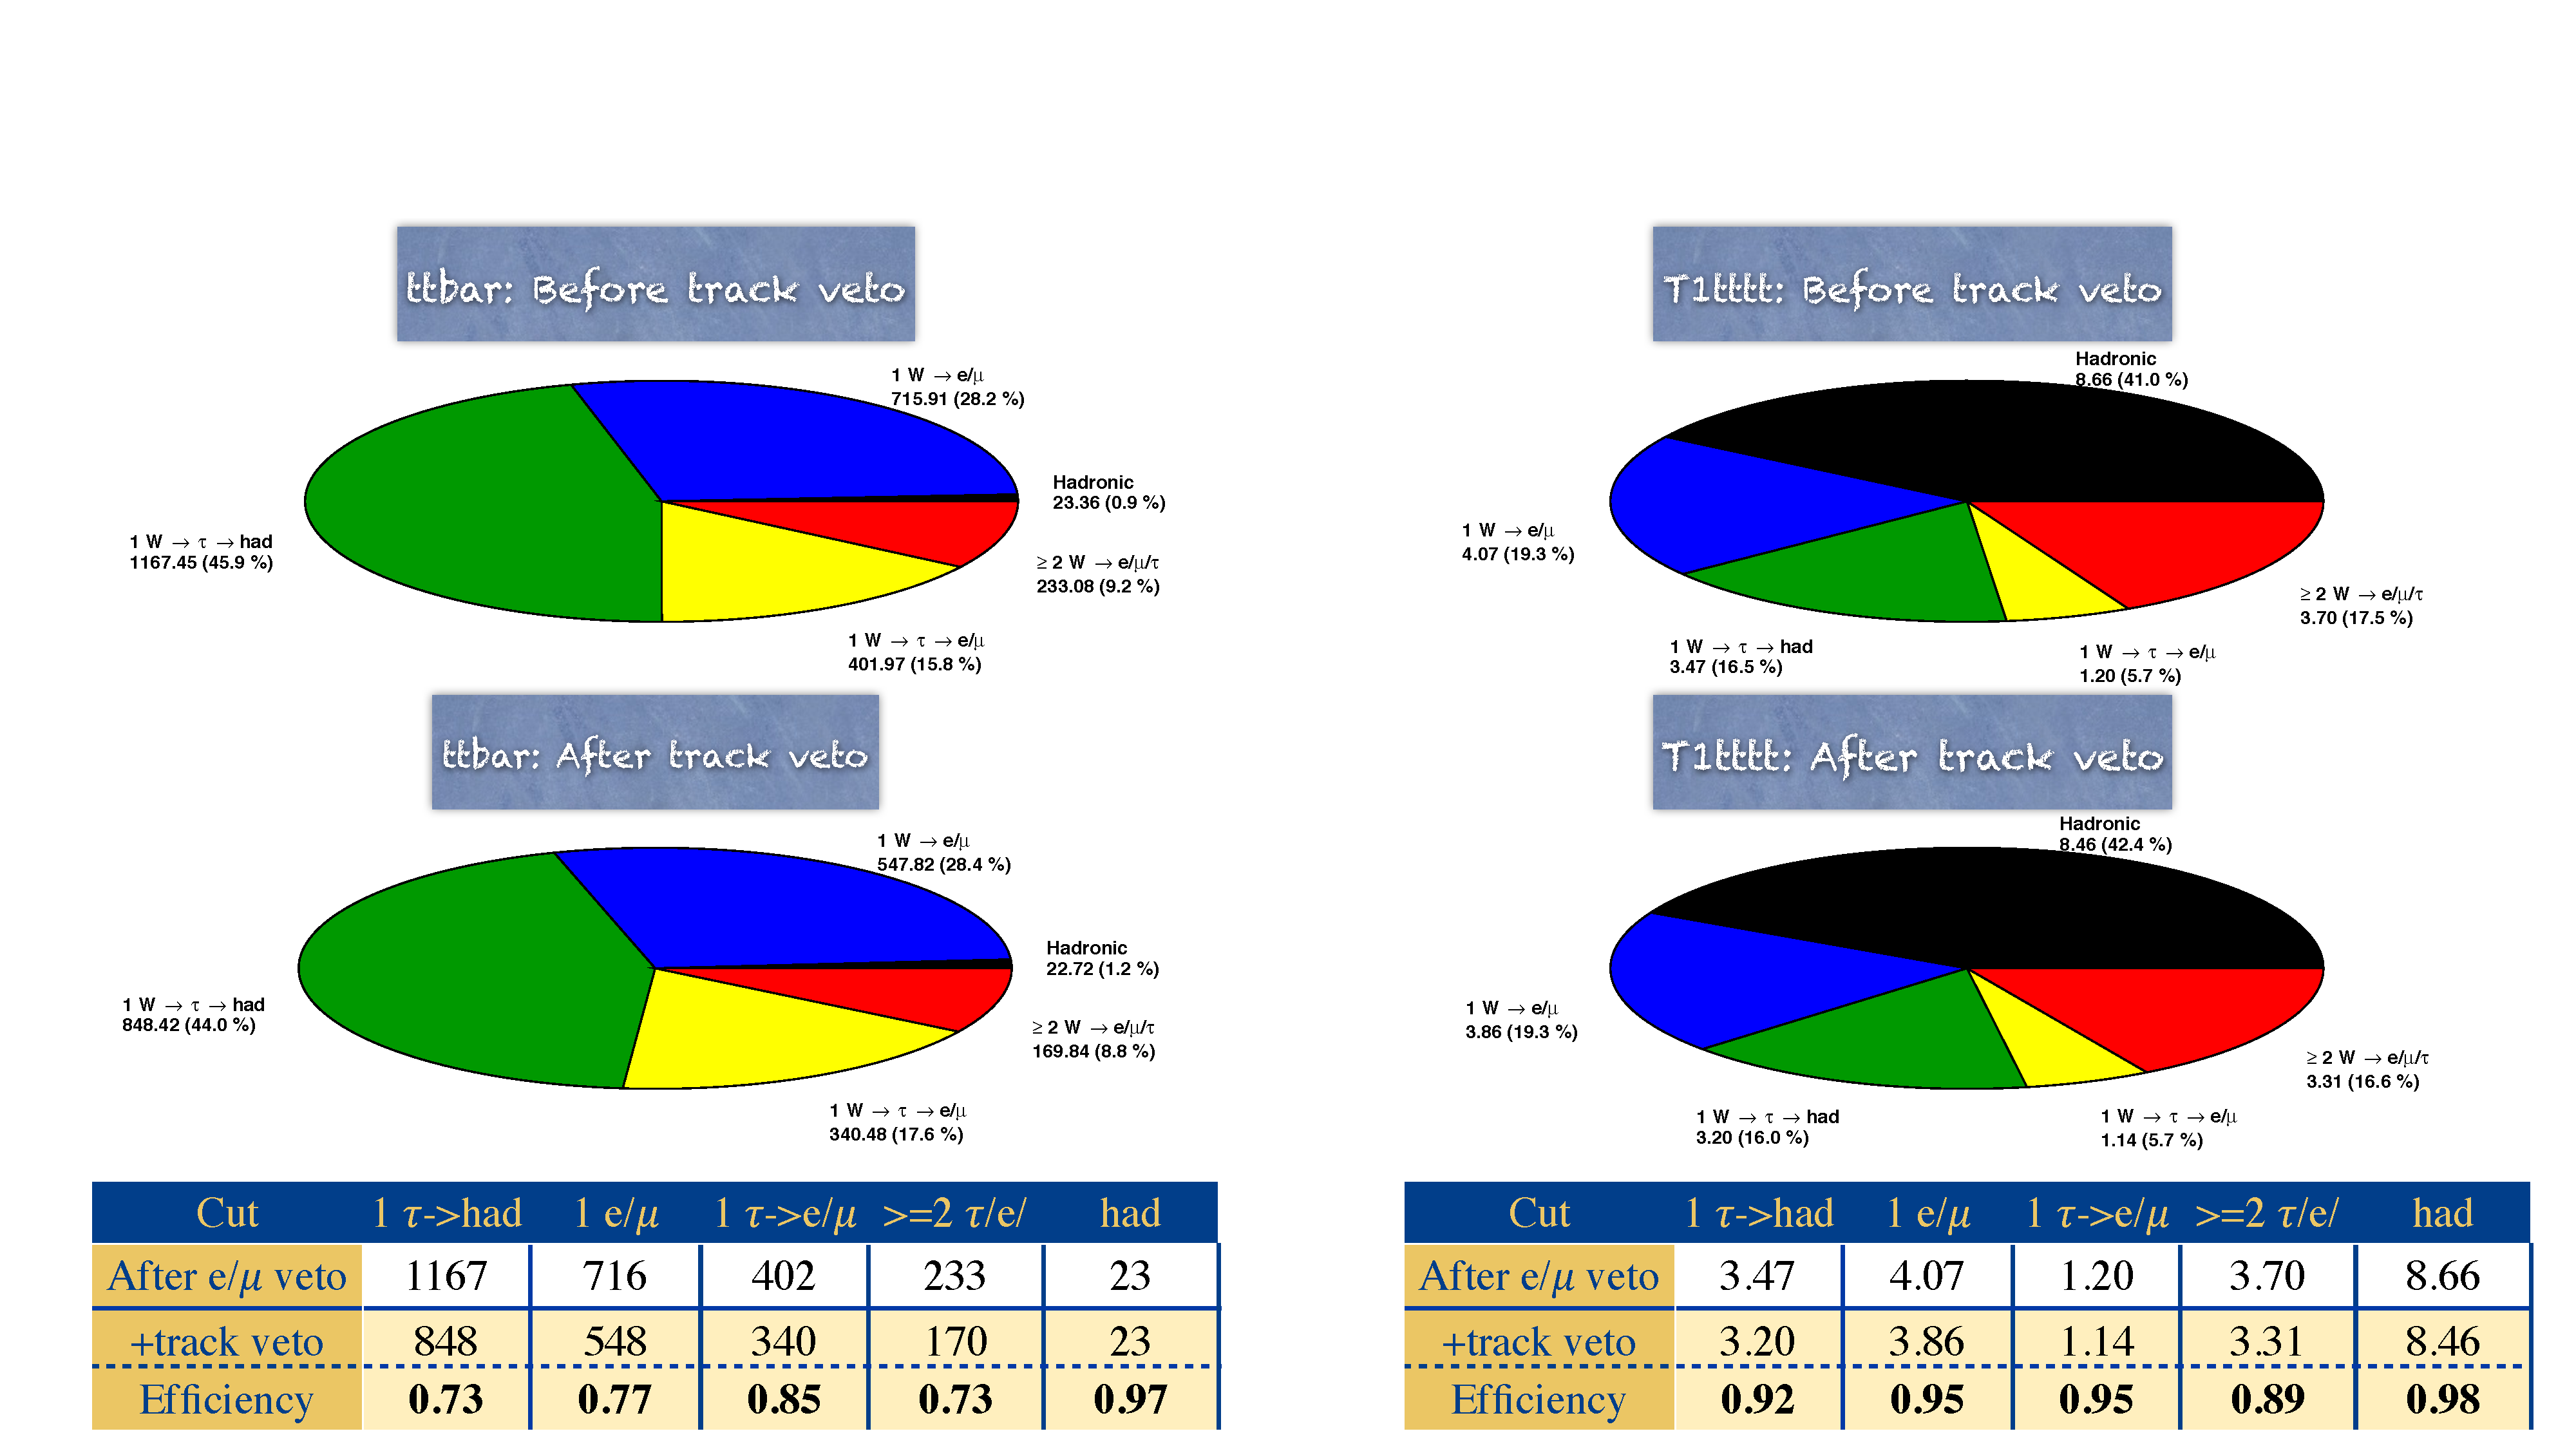
\includegraphics[width=\textwidth]{figures/jacks_Studies/rejection_slide}
  \end{figure}
\end{frame}


\begin{frame}
\frametitle{Parametrization of Efficiencies}
  \begin{columns}
    \begin{column}{0.5\textwidth}
     \centering
     Old
     \begin{itemize}




        \item Isolation
   \begin{itemize}
    \item \HT \MHT \NJets (\BTags)
   \end{itemize}
   \item Reconstruction
   \begin{itemize}
    \item \HT \MHT \NJets (\BTags)
   \end{itemize}
   \item Acceptance
   \begin{itemize}
    \item \MHT \NJets (\BTags)
   \end{itemize}
   \item Purity (only electron CS)
   \begin{itemize}
    \item \MHT \NJets
   \end{itemize}
      \item Di-lep contamination
   \begin{itemize}
    \item \MHT \NJets
   \end{itemize}
   \item Di-lep efficiency
   \begin{itemize}
    \item \NJets
   \end{itemize}
   \item \mt cut efficiency
   \begin{itemize}
    \item \NJets
   \end{itemize}
     \end{itemize}
    \end{column}
    \begin{column}{0.5\textwidth}
      \centering
      New
             \begin{itemize}


        \item Isolation
   \begin{itemize}
    \item Lep \pt Activity
   \end{itemize}
   \item Reconstruction
   \begin{itemize}
    \item Activity
   \end{itemize}
   \item Acceptance
   \begin{itemize}
    \item \BTags \NJets
   \end{itemize}
   \item Purity (only electron CS)
   \begin{itemize}
    \item \MHT \NJets
   \end{itemize}
      \item Di-lep contamination
   \begin{itemize}
    \item \NJets
   \end{itemize}
   \item Di-lep efficiency
   \begin{itemize}
    \item \NJets
   \end{itemize}
   \item \mt cut efficiency
   \begin{itemize}
    \item Activity
   \end{itemize}
     \end{itemize}
    \end{column}
  \end{columns}
\end{frame}
\subsection{Closure}
\begin{frame}
 \begin{center}
    {\Large Closure Muon Control Sample}
  \end{center}
\end{frame}
\begin{frame}
\frametitle{Muon Control Sample: Closure Test \HT \& \MHT}
  \begin{columns}
    \begin{column}{0.5\textwidth}
     \centering
      \begin{overpic}[width=0.70\textwidth]{figures/deltaphicut/Closure_Old_Parametrization/Closure__HT__MuPrMTWDiLep_vs_MCEx__Baseline.pdf}\put(100,60){\rotatebox{-90}{\scriptsize Old Parametrization Variables}}
     \end{overpic}
      \begin{overpic}[width=0.70\textwidth]{figures/deltaphicut/Closure_Old_Parametrization/Closure__MHT__MuPrMTWDiLep_vs_MCEx__Baseline.pdf}
     \end{overpic}
    \end{column}
    \begin{column}{0.5\textwidth}
      \centering
      \begin{overpic}[width=0.70\textwidth]{figures/deltaphicut/Closure_New_Parametrization/Closure__HT__MuPrMTWDiLep_vs_MCEx__Baseline.pdf} \put(100,60){\rotatebox{-90}{\scriptsize New Parametrization Variables}}     \end{overpic}
      \centering
      \begin{overpic}[width=0.70\textwidth]{figures/deltaphicut/Closure_New_Parametrization/Closure__MHT__MuPrMTWDiLep_vs_MCEx__Baseline}     \end{overpic}
    \end{column}
  \end{columns}
\end{frame}

\begin{frame}
\frametitle{Muon Control Sample: Closure Test \NJets \& \BTags}
  \begin{columns}
    \begin{column}{0.5\textwidth}
     \centering
      \begin{overpic}[width=0.70\textwidth]{figures/deltaphicut/Closure_Old_Parametrization/Closure__BTags__MuPrMTWDiLep_vs_MCEx__Baseline.pdf} \put(100,60){\rotatebox{-90}{\scriptsize Old Parametrization Variables}}
     \end{overpic}
      \begin{overpic}[width=0.70\textwidth]{figures/deltaphicut/Closure_Old_Parametrization/Closure__NJets__MuPrMTWDiLep_vs_MCEx__Baseline.pdf}
     \end{overpic}
    \end{column}
    \begin{column}{0.5\textwidth}
      \centering
      \begin{overpic}[width=0.70\textwidth]{figures/deltaphicut/Closure_New_Parametrization/Closure__BTags__MuPrMTWDiLep_vs_MCEx__Baseline.pdf}  \put(100,60){\rotatebox{-90}{\scriptsize New Parametrization Variables}}
      \end{overpic}
      \centering
      \begin{overpic}[width=0.70\textwidth]{figures/deltaphicut/Closure_New_Parametrization/Closure__NJets__MuPrMTWDiLep_vs_MCEx__Baseline}     \end{overpic}
    \end{column}
  \end{columns}
\end{frame}

\begin{frame}
 \begin{center}
    {\Large Closure Eletron Control Sample}
  \end{center}
\end{frame}

\begin{frame}
\frametitle{Electron Control Sample: Closure Test \HT \& \MHT}
  \begin{columns}
    \begin{column}{0.5\textwidth}
     \centering
      \begin{overpic}[width=0.70\textwidth]{figures/deltaphicut/Closure_Old_Parametrization/Closure__HT__ElecPrMTWDiLep_vs_MCEx__Baseline.pdf}\put(100,60){\rotatebox{-90}{\scriptsize Old Parametrization Variables}}
     \end{overpic}
      \begin{overpic}[width=0.70\textwidth]{figures/deltaphicut/Closure_Old_Parametrization/Closure__MHT__ElecPrMTWDiLep_vs_MCEx__Baseline.pdf}
     \end{overpic}
    \end{column}
    \begin{column}{0.5\textwidth}
      \centering
      \begin{overpic}[width=0.70\textwidth]{figures/deltaphicut/Closure_New_Parametrization/Closure__HT__ElecPrMTWDiLep_vs_MCEx__Baseline.pdf}  \put(100,60){\rotatebox{-90}{\scriptsize New Parametrization Variables}}   \end{overpic}
      \centering
      \begin{overpic}[width=0.70\textwidth]{figures/deltaphicut/Closure_New_Parametrization/Closure__MHT__ElecPrMTWDiLep_vs_MCEx__Baseline}     \end{overpic}
    \end{column}
  \end{columns}
\end{frame}

\begin{frame}
\frametitle{Electron Control Sample Closure Test \NJets \& \BTags}
  \begin{columns}
    \begin{column}{0.5\textwidth}
     \centering
      \begin{overpic}[width=0.70\textwidth]{figures/deltaphicut/Closure_Old_Parametrization/Closure__BTags__ElecPrMTWDiLep_vs_MCEx__Baseline.pdf} \put(100,60){\rotatebox{-90}{\scriptsize Old Parametrization Variables}}
     \end{overpic}
      \begin{overpic}[width=0.70\textwidth]{figures/deltaphicut/Closure_Old_Parametrization/Closure__NJets__ElecPrMTWDiLep_vs_MCEx__Baseline.pdf}
     \end{overpic}
    \end{column}
    \begin{column}{0.5\textwidth}
      \centering
      \begin{overpic}[width=0.70\textwidth]{figures/deltaphicut/Closure_New_Parametrization/Closure__BTags__ElecPrMTWDiLep_vs_MCEx__Baseline.pdf}  \put(100,60){\rotatebox{-90}{\scriptsize New Parametrization Variables}}   \end{overpic}
      \centering
      \begin{overpic}[width=0.70\textwidth]{figures/deltaphicut/Closure_New_Parametrization/Closure__NJets__ElecPrMTWDiLep_vs_MCEx__Baseline}     \end{overpic}
    \end{column}
  \end{columns}
\end{frame}



\begin{frame}
 \begin{center}
    {\Large Combined Electron and Muon Control Sample Closure}
  \end{center}
\end{frame}
\begin{frame}
\frametitle{Muon \& Elec Control Sample Combined Closure}
  \begin{columns}
    \begin{column}{0.5\textwidth}
     \centering
      \begin{overpic}[width=0.70\textwidth]{figures/deltaphicut/Closure_New_Parametrization/Closure_Combined__HT__MCEx_vs_MuPrMTWDiLep+ElecPrMTWDiLep__Baseline.pdf}
     \end{overpic}
     \begin{overpic}[width=0.70\textwidth]{figures/deltaphicut/Closure_New_Parametrization/Closure_Combined__BTags__MCEx_vs_MuPrMTWDiLep+ElecPrMTWDiLep__Baseline.pdf}
     \end{overpic}
    \end{column}
    \begin{column}{0.5\textwidth}
      \centering
      \begin{overpic}[width=0.70\textwidth]{figures/deltaphicut/Closure_New_Parametrization/Closure_Combined__MHT__MCEx_vs_MuPrMTWDiLep+ElecPrMTWDiLep__Baseline.pdf}     \end{overpic}
      \centering
      \begin{overpic}[width=0.70\textwidth]{figures/deltaphicut/Closure_New_Parametrization/Closure_Combined__NJets__MCEx_vs_MuPrMTWDiLep+ElecPrMTWDiLep__Baseline.pdf}     \end{overpic}
    \end{column}
  \end{columns}
\end{frame}

\begin{frame}
 \begin{center}
    {\Large Separate Closure Muon Control Sample}
  \end{center}
\end{frame}

\subsection{Lost Lepton equations (reminder)}
\begin{frame}
 \begin{equation}
 \rm !ISO^{\mu} = {\rm CS}\cdot \frac{1-\epsilon_{\rm ISO}^{\mu}}{\epsilon_{\rm ISO}^{\mu}}
    %%   \rm !ISO^{\mu}} = {\rm CS}\cdot \frac{1-\epsilon_{\rm ISO}^{\mu}}{\epsilon_{\rm ISO}^{\mu}}
\label{eq:isolation_muon}
\end{equation}
\begin{equation}
 {\rm !Reco^{\mu}} = {\rm CS}\cdot \frac{1}{\epsilon_{\rm ISO}^{\mu}} \cdot \frac{1-\epsilon_{\rm Reco}^{\mu}}{\epsilon_{\rm Reco}^{\mu}}
\label{eq:reconstruction_muon}
\end{equation}
\begin{equation}
 {\rm !Acc^{\mu}} = {\rm CS}\cdot \frac{1}{\epsilon_{\rm ISO}^{\mu}}\cdot \frac{1}{\epsilon_{\rm Reco}^{\mu}} \cdot \frac{1-\epsilon^{\mu}_{Acc}}{\epsilon^{\mu}_{Acc}}
\label{eq:acceptance_muon}
\end{equation}
\begin{equation}
{\rm !Acc^{e}} = {\rm CS}\cdot \frac{1}{\epsilon_{\rm ISO}^{\mu}}\cdot \frac{1}{\epsilon_{\rm Reco}^{\mu}}  \cdot \frac{1 - \epsilon^{e}_{Acc}}{\epsilon^{\mu}_{Acc}}
 \label{eq:elec_acc}
\end{equation}
\begin{equation}
{\rm !Reco^{e}} = {\rm CS}\cdot \frac{1}{\epsilon_{\rm ISO}^{\mu}}\cdot \frac{1-\epsilon_{\rm Reco}^{e}}{\epsilon_{\rm Reco}^{\mu}}  \cdot \frac{\epsilon^{e}_{Acc}}{\epsilon^{\mu}_{Acc}}
 \label{eq:elec_reco}
\end{equation}
\begin{equation}
{\rm !ISO^{e}} = {\rm CS}\cdot \frac{1-\epsilon_{\rm ISO}^{e}}{\epsilon_{\rm ISO}^{\mu}} \cdot \frac{\epsilon^{e}_{Reco}}{\epsilon^{\mu}_{Reco}} \cdot \frac{\epsilon^{e}_{Acc}}{\epsilon^{\mu}_{Acc}}
\label{eq:elec_iso}
\end{equation}
\begin{itemize}
 \item Keep in mind the dependency of each step! Non-Closure propagates to all following precitions!
\end{itemize}

\end{frame}
\subsection{Muon CS Separate Closure}

\begin{frame}
 \frametitle{Muon Control Sample: Remaining Non-Closure $\mu$ Iso}
   \begin{columns}
    \begin{column}{0.5\textwidth}
     \centering
      \begin{overpic}[width=0.70\textwidth]{figures/deltaphicut/separate_closure/Mu_Closure_test__HT__MuExIso_vs_MuCSPrIso__Baseline.pdf}
     \end{overpic}
      \begin{overpic}[width=0.70\textwidth]{figures/deltaphicut/separate_closure/Mu_Closure_test__BTags__MuExIso_vs_MuCSPrIso__Baseline.pdf}
     \end{overpic}
    \end{column}
    \begin{column}{0.5\textwidth}
      \centering
      \begin{overpic}[width=0.70\textwidth]{figures/deltaphicut/separate_closure/Mu_Closure_test__MHT__MuExIso_vs_MuCSPrIso__Baseline.pdf}     \end{overpic}
      \centering
      \begin{overpic}[width=0.70\textwidth]{figures/deltaphicut/separate_closure/Mu_Closure_test__NJets__MuExIso_vs_MuCSPrIso__Baseline.pdf}     \end{overpic}
    \end{column}
  \end{columns}
\end{frame}
\begin{frame}
 \frametitle{Muon Control Sample: Remaining Non-Closure $\mu$ Reco}
   \begin{columns}
    \begin{column}{0.5\textwidth}
     \centering
      \begin{overpic}[width=0.70\textwidth]{figures/deltaphicut/separate_closure/Mu_Closure_test__HT__MuExReco_vs_MuCSPrReco__Baseline.pdf}
     \end{overpic}
      \begin{overpic}[width=0.70\textwidth]{figures/deltaphicut/separate_closure/Mu_Closure_test__BTags__MuExReco_vs_MuCSPrReco__Baseline.pdf}
     \end{overpic}
    \end{column}
    \begin{column}{0.5\textwidth}
      \centering
      \begin{overpic}[width=0.70\textwidth]{figures/deltaphicut/separate_closure/Mu_Closure_test__MHT__MuExReco_vs_MuCSPrReco__Baseline.pdf}     \end{overpic}
      \centering
      \begin{overpic}[width=0.70\textwidth]{figures/deltaphicut/separate_closure/Mu_Closure_test__NJets__MuExReco_vs_MuCSPrReco__Baseline.pdf}     \end{overpic}
    \end{column}
  \end{columns}
\end{frame}


\begin{frame}
 \frametitle{Muon Control Sample: Remaining Non-Closure $\mu$ Acc}
   \begin{columns}
    \begin{column}{0.5\textwidth}
     \centering
      \begin{overpic}[width=0.70\textwidth]{figures/deltaphicut/separate_closure/Mu_Closure_test__HT__MuExAcc_vs_MuCSPrAcc__Baseline.pdf}
     \end{overpic}
      \begin{overpic}[width=0.70\textwidth]{figures/deltaphicut/separate_closure/Mu_Closure_test__BTags__MuExAcc_vs_MuCSPrAcc__Baseline.pdf}
     \end{overpic}
    \end{column}
    \begin{column}{0.5\textwidth}
      \centering
      \begin{overpic}[width=0.70\textwidth]{figures/deltaphicut/separate_closure/Mu_Closure_test__MHT__MuExAcc_vs_MuCSPrAcc__Baseline.pdf}     \end{overpic}
      \centering
      \begin{overpic}[width=0.70\textwidth]{figures/deltaphicut/separate_closure/Mu_Closure_test__NJets__MuExAcc_vs_MuCSPrAcc__Baseline.pdf}     \end{overpic}
    \end{column}
  \end{columns}
\end{frame}


\begin{frame}
 \frametitle{Muon Control Sample: Remaining Non-Closure e Acc}
   \begin{columns}
    \begin{column}{0.5\textwidth}
     \centering
      \begin{overpic}[width=0.70\textwidth]{figures/deltaphicut/separate_closure/Elec_Closure_test__HT__ElecExAcc_vs_MuCSPrAcc__Baseline.pdf}
     \end{overpic}
      \begin{overpic}[width=0.70\textwidth]{figures/deltaphicut/separate_closure/Elec_Closure_test__BTags__ElecExAcc_vs_MuCSPrAcc__Baseline.pdf}
     \end{overpic}
    \end{column}
    \begin{column}{0.5\textwidth}
      \centering
      \begin{overpic}[width=0.70\textwidth]{figures/deltaphicut/separate_closure/Elec_Closure_test__MHT__ElecExAcc_vs_MuCSPrAcc__Baseline.pdf}     \end{overpic}
      \centering
      \begin{overpic}[width=0.70\textwidth]{figures/deltaphicut/separate_closure/Elec_Closure_test__NJets__ElecExAcc_vs_MuCSPrAcc__Baseline.pdf}     \end{overpic}
    \end{column}
  \end{columns}
\end{frame}


\begin{frame}
 \frametitle{Muon Control Sample: Remaining Non-Closure e Reco}
   \begin{columns}
    \begin{column}{0.5\textwidth}
     \centering
      \begin{overpic}[width=0.70\textwidth]{figures/deltaphicut/separate_closure/Elec_Closure_test__HT__ElecExReco_vs_MuCSPrReco__Baseline.pdf}
     \end{overpic}
      \begin{overpic}[width=0.70\textwidth]{figures/deltaphicut/separate_closure/Elec_Closure_test__BTags__ElecExReco_vs_MuCSPrReco__Baseline.pdf}
     \end{overpic}
    \end{column}
    \begin{column}{0.5\textwidth}
      \centering
      \begin{overpic}[width=0.70\textwidth]{figures/deltaphicut/separate_closure/Elec_Closure_test__MHT__ElecExReco_vs_MuCSPrReco__Baseline.pdf}     \end{overpic}
      \centering
      \begin{overpic}[width=0.70\textwidth]{figures/deltaphicut/separate_closure/Elec_Closure_test__NJets__ElecExReco_vs_MuCSPrReco__Baseline.pdf}     \end{overpic}
    \end{column}
  \end{columns}
\end{frame}


\begin{frame}
 \frametitle{Muon Control Sample: Remaining Non-Closure e Iso}
   \begin{columns}
    \begin{column}{0.5\textwidth}
     \centering
      \begin{overpic}[width=0.70\textwidth]{figures/deltaphicut/separate_closure/Elec_Closure_test__HT__ElecExIso_vs_MuCSPrIso__Baseline.pdf}
     \end{overpic}
      \begin{overpic}[width=0.70\textwidth]{figures/deltaphicut/separate_closure/Elec_Closure_test__BTags__ElecExIso_vs_MuCSPrIso__Baseline.pdf}
     \end{overpic}
    \end{column}
    \begin{column}{0.5\textwidth}
      \centering
      \begin{overpic}[width=0.70\textwidth]{figures/deltaphicut/separate_closure/Elec_Closure_test__MHT__ElecExIso_vs_MuCSPrIso__Baseline.pdf}     \end{overpic}
      \centering
      \begin{overpic}[width=0.70\textwidth]{figures/deltaphicut/separate_closure/Elec_Closure_test__NJets__ElecExIso_vs_MuCSPrIso__Baseline.pdf}     \end{overpic}
    \end{column}
  \end{columns}
\end{frame}

\subsection{Electron CS Separate Closure}
\begin{frame}
 \begin{center}
    {\Large Separate Closure Eletron Control Sample}
  \end{center}
\end{frame}


\begin{frame}
 \frametitle{Elec Control Sample: Remaining Non-Closure e Iso}
   \begin{columns}
    \begin{column}{0.5\textwidth}
     \centering
      \begin{overpic}[width=0.70\textwidth]{figures/deltaphicut/separate_closure/Elec_Closure_test__HT__ElecExIso_vs_ElecCSPrIso__Baseline.pdf}
     \end{overpic}
      \begin{overpic}[width=0.70\textwidth]{figures/deltaphicut/separate_closure/Elec_Closure_test__BTags__ElecExIso_vs_ElecCSPrIso__Baseline.pdf}
     \end{overpic}
    \end{column}
    \begin{column}{0.5\textwidth}
      \centering
      \begin{overpic}[width=0.70\textwidth]{figures/deltaphicut/separate_closure/Elec_Closure_test__MHT__ElecExIso_vs_ElecCSPrIso__Baseline.pdf}     \end{overpic}
      \centering
      \begin{overpic}[width=0.70\textwidth]{figures/deltaphicut/separate_closure/Elec_Closure_test__NJets__ElecExIso_vs_ElecCSPrIso__Baseline.pdf}     \end{overpic}
    \end{column}
  \end{columns}
\end{frame}



\begin{frame}
 \frametitle{Elec Control Sample: Remaining Non-Closure e Reco}
   \begin{columns}
    \begin{column}{0.5\textwidth}
     \centering
      \begin{overpic}[width=0.70\textwidth]{figures/deltaphicut/separate_closure/Elec_Closure_test__HT__ElecExReco_vs_ElecCSPrReco__Baseline.pdf}
     \end{overpic}
      \begin{overpic}[width=0.70\textwidth]{figures/deltaphicut/separate_closure/Elec_Closure_test__BTags__ElecExReco_vs_ElecCSPrReco__Baseline.pdf}
     \end{overpic}
    \end{column}
    \begin{column}{0.5\textwidth}
      \centering
      \begin{overpic}[width=0.70\textwidth]{figures/deltaphicut/separate_closure/Elec_Closure_test__MHT__ElecExReco_vs_ElecCSPrReco__Baseline.pdf}     \end{overpic}
      \centering
      \begin{overpic}[width=0.70\textwidth]{figures/deltaphicut/separate_closure/Elec_Closure_test__NJets__ElecExReco_vs_ElecCSPrReco__Baseline.pdf}     \end{overpic}
    \end{column}
  \end{columns}
\end{frame}





\begin{frame}
 \frametitle{Elec Control Sample: Remaining Non-Closure e Acc}
   \begin{columns}
    \begin{column}{0.5\textwidth}
     \centering
      \begin{overpic}[width=0.70\textwidth]{figures/deltaphicut/separate_closure/Elec_Closure_test__HT__ElecExAcc_vs_ElecCSPrAcc__Baseline.pdf}
     \end{overpic}
      \begin{overpic}[width=0.70\textwidth]{figures/deltaphicut/separate_closure/Elec_Closure_test__BTags__ElecExAcc_vs_ElecCSPrAcc__Baseline.pdf}
     \end{overpic}
    \end{column}
    \begin{column}{0.5\textwidth}
      \centering
      \begin{overpic}[width=0.70\textwidth]{figures/deltaphicut/separate_closure/Elec_Closure_test__MHT__ElecExAcc_vs_ElecCSPrAcc__Baseline.pdf}     \end{overpic}
      \centering
      \begin{overpic}[width=0.70\textwidth]{figures/deltaphicut/separate_closure/Elec_Closure_test__NJets__ElecExAcc_vs_ElecCSPrAcc__Baseline.pdf}     \end{overpic}
    \end{column}
  \end{columns}
\end{frame}


\begin{frame}
 \frametitle{Elec Control Sample: Remaining Non-Closure $\mu$ Acc}
   \begin{columns}
    \begin{column}{0.5\textwidth}
     \centering
      \begin{overpic}[width=0.70\textwidth]{figures/deltaphicut/separate_closure/Mu_Closure_test__HT__MuExAcc_vs_ElecCSPrAcc__Baseline.pdf}
     \end{overpic}
      \begin{overpic}[width=0.70\textwidth]{figures/deltaphicut/separate_closure/Mu_Closure_test__BTags__MuExAcc_vs_ElecCSPrAcc__Baseline.pdf}
     \end{overpic}
    \end{column}
    \begin{column}{0.5\textwidth}
      \centering
      \begin{overpic}[width=0.70\textwidth]{figures/deltaphicut/separate_closure/Mu_Closure_test__MHT__MuExAcc_vs_ElecCSPrAcc__Baseline.pdf}     \end{overpic}
      \centering
      \begin{overpic}[width=0.70\textwidth]{figures/deltaphicut/separate_closure/Mu_Closure_test__NJets__MuExAcc_vs_ElecCSPrAcc__Baseline.pdf}     \end{overpic}
    \end{column}
  \end{columns}
\end{frame}




\begin{frame}
 \frametitle{Elec Control Sample: Remaining Non-Closure $\mu$ Reco}
   \begin{columns}
    \begin{column}{0.5\textwidth}
     \centering
      \begin{overpic}[width=0.70\textwidth]{figures/deltaphicut/separate_closure/Mu_Closure_test__HT__MuExReco_vs_ElecCSPrReco__Baseline.pdf}
     \end{overpic}
      \begin{overpic}[width=0.70\textwidth]{figures/deltaphicut/separate_closure/Mu_Closure_test__BTags__MuExReco_vs_ElecCSPrReco__Baseline.pdf}
     \end{overpic}
    \end{column}
    \begin{column}{0.5\textwidth}
      \centering
      \begin{overpic}[width=0.70\textwidth]{figures/deltaphicut/separate_closure/Mu_Closure_test__MHT__MuExReco_vs_ElecCSPrReco__Baseline.pdf}     \end{overpic}
      \centering
      \begin{overpic}[width=0.70\textwidth]{figures/deltaphicut/separate_closure/Mu_Closure_test__NJets__MuExReco_vs_ElecCSPrReco__Baseline.pdf}     \end{overpic}
    \end{column}
  \end{columns}
\end{frame}



\begin{frame}
 \frametitle{Elec Control Sample: Remaining Non-Closure $\mu$ Iso}
   \begin{columns}
    \begin{column}{0.5\textwidth}
     \centering
      \begin{overpic}[width=0.70\textwidth]{figures/deltaphicut/separate_closure/Mu_Closure_test__HT__MuExIso_vs_ElecCSPrIso__Baseline.pdf}
     \end{overpic}
      \begin{overpic}[width=0.70\textwidth]{figures/deltaphicut/separate_closure/Mu_Closure_test__BTags__MuExIso_vs_ElecCSPrIso__Baseline.pdf}
     \end{overpic}
    \end{column}
    \begin{column}{0.5\textwidth}
      \centering
      \begin{overpic}[width=0.70\textwidth]{figures/deltaphicut/separate_closure/Mu_Closure_test__MHT__MuExIso_vs_ElecCSPrIso__Baseline.pdf}     \end{overpic}
      \centering
      \begin{overpic}[width=0.70\textwidth]{figures/deltaphicut/separate_closure/Mu_Closure_test__NJets__MuExIso_vs_ElecCSPrIso__Baseline.pdf}     \end{overpic}
    \end{column}
  \end{columns}
\end{frame}

\subsection{Muon Efficiencies}
\begin{frame}
 \begin{center}
    {\Large Efficiencies: Muon}
  \end{center}
\end{frame}

\begin{frame}
\frametitle{$\mu$ iso}
   \begin{columns}
    \begin{column}{0.33\textwidth}
     \centering
      \begin{overpic}[width=1.00\textwidth]{figures/deltaphicut/efficiencies/MuIsoHT1D.pdf}
     \end{overpic}
      \begin{overpic}[width=1.00\textwidth]{figures/deltaphicut/efficiencies/MuIsoNJets1D.pdf}
     \end{overpic}
    \end{column}
    \begin{column}{0.33\textwidth}
      \centering
      \begin{overpic}[width=1.00\textwidth]{figures/deltaphicut/efficiencies/MuIsoMHT1D.pdf}      \end{overpic}
      \centering
      \begin{overpic}[width=1.00\textwidth]{figures/deltaphicut/efficiencies/MuIsoPT.pdf}      \end{overpic}
    \end{column}
    \begin{column}{0.33\textwidth}
     \centering
      \begin{overpic}[width=1.00\textwidth]{figures/deltaphicut/efficiencies/MuIsoBTag1D.pdf}      \end{overpic}
      \begin{overpic}[width=1.00\textwidth]{figures/deltaphicut/efficiencies/MuIsoActivity.pdf} \end{overpic}

    \end{column}

  \end{columns}
\end{frame}

\begin{frame}
 \frametitle{$\mu$ iso used parametization and binnning}
\centering
      \begin{overpic}[width=0.90\textwidth]{figures/deltaphicut/efficiencies/MuIsoPTActivity.pdf}
     \end{overpic}
\end{frame}

\begin{frame}
\frametitle{$\mu$ reco}
   \begin{columns}
    \begin{column}{0.33\textwidth}
     \centering
      \begin{overpic}[width=1.00\textwidth]{figures/deltaphicut/efficiencies/MuRecoHT1D.pdf}
     \end{overpic}
      \begin{overpic}[width=1.00\textwidth]{figures/deltaphicut/efficiencies/MuRecoNJets1D.pdf}
     \end{overpic}
    \end{column}
    \begin{column}{0.33\textwidth}
      \centering
      \begin{overpic}[width=1.00\textwidth]{figures/deltaphicut/efficiencies/MuRecoMHT1D.pdf}      \end{overpic}
      \centering
      \begin{overpic}[width=1.00\textwidth]{figures/deltaphicut/efficiencies/MuRecoPT.pdf}      \end{overpic}
    \end{column}
    \begin{column}{0.33\textwidth}
     \centering
      \begin{overpic}[width=1.00\textwidth]{figures/deltaphicut/efficiencies/MuRecoBTag1D.pdf}      \end{overpic}
         \begin{overpic}[width=1.00\textwidth]{figures/deltaphicut/efficiencies/MuRecoActivity.pdf} \end{overpic}

    \end{column}

  \end{columns}
\end{frame}

\begin{frame}
 \frametitle{$\mu$ reco used parametization and binnning}
\centering
      \begin{overpic}[width=0.90\textwidth]{figures/deltaphicut/efficiencies/MuRecoActivity.pdf}
     \end{overpic}
\end{frame}

\begin{frame}
\frametitle{$\mu$ acc}
   \begin{columns}
    \begin{column}{0.33\textwidth}
     \centering
      \begin{overpic}[width=1.00\textwidth]{figures/deltaphicut/efficiencies/MuAccHT1D.pdf}
     \end{overpic}
      \begin{overpic}[width=1.00\textwidth]{figures/deltaphicut/efficiencies/MuAccNJets1D.pdf}
     \end{overpic}
    \end{column}
    \begin{column}{0.33\textwidth}
      \centering
      \begin{overpic}[width=1.00\textwidth]{figures/deltaphicut/efficiencies/MuAccMHT1D.pdf}      \end{overpic}
      \begin{overpic}[width=1.00\textwidth]{figures/deltaphicut/efficiencies/MuAccActivity.pdf} \end{overpic}
      \centering
    \end{column}
    \begin{column}{0.33\textwidth}
     \centering
      \begin{overpic}[width=1.00\textwidth]{figures/deltaphicut/efficiencies/MuAccBTag1D.pdf}      \end{overpic}
\begin{overpic}[width=1.00\textwidth]{figures/deltaphicut/efficiencies/MuAccPT.pdf}      \end{overpic}

    \end{column}

  \end{columns}
\end{frame}

\begin{frame}
 \frametitle{$\mu$ acc used parametization and binnning}
\centering
      \begin{overpic}[width=0.90\textwidth]{figures/deltaphicut/efficiencies/MuAccBTagNJets.pdf}
     \end{overpic}
\end{frame}

\begin{frame}
\frametitle{$\mu$ Purity}
   \begin{columns}
    \begin{column}{0.33\textwidth}
     \centering
      \begin{overpic}[width=1.00\textwidth]{figures/deltaphicut/efficiencies/MuPurityHT1D.pdf}
     \end{overpic}
      \begin{overpic}[width=1.00\textwidth]{figures/deltaphicut/efficiencies/MuPurityNJets1D.pdf}
     \end{overpic}
    \end{column}
    \begin{column}{0.33\textwidth}
      \centering
      \begin{overpic}[width=1.00\textwidth]{figures/deltaphicut/efficiencies/MuPurityMHT1D.pdf}      \end{overpic}
      \begin{overpic}[width=1.00\textwidth]{figures/deltaphicut/efficiencies/MuPurityActivity.pdf} \end{overpic}
      \centering
    \end{column}
    \begin{column}{0.33\textwidth}
     \centering
      \begin{overpic}[width=1.00\textwidth]{figures/deltaphicut/efficiencies/MuPurityBTag1D.pdf}      \end{overpic}
\begin{overpic}[width=1.00\textwidth]{figures/deltaphicut/efficiencies/MuPurityPT.pdf}      \end{overpic}

    \end{column}

  \end{columns}
\end{frame}


\begin{frame}
 \begin{center}
    {\Large $\mu$ purity not corrected for!}
  \end{center}
\end{frame}

\begin{frame}
\frametitle{$\mu$ \mt-cut}
   \begin{columns}
    \begin{column}{0.33\textwidth}
     \centering
      \begin{overpic}[width=1.00\textwidth]{figures/deltaphicut/efficiencies/MuMTWHT1D.pdf}
     \end{overpic}
      \begin{overpic}[width=1.00\textwidth]{figures/deltaphicut/efficiencies/MuMTWNJets1D.pdf}
     \end{overpic}
    \end{column}
    \begin{column}{0.33\textwidth}
      \centering
      \begin{overpic}[width=1.00\textwidth]{figures/deltaphicut/efficiencies/MuMTWMHT1D.pdf}      \end{overpic}
      \begin{overpic}[width=1.00\textwidth]{figures/deltaphicut/efficiencies/MuMTWActivity.pdf} \end{overpic}
      \centering
    \end{column}
    \begin{column}{0.33\textwidth}
     \centering
      \begin{overpic}[width=1.00\textwidth]{figures/deltaphicut/efficiencies/MuMTWBTag1D.pdf}      \end{overpic}
\begin{overpic}[width=1.00\textwidth]{figures/deltaphicut/efficiencies/MuMTWPT.pdf}      \end{overpic}

    \end{column}

  \end{columns}
\end{frame}


\begin{frame}
 \frametitle{$\mu$ \mt-cut used parametization and binnning}
\centering
      \begin{overpic}[width=0.90\textwidth]{figures/deltaphicut/efficiencies/MuMTWPTActivity.pdf}
     \end{overpic}
\end{frame}


\begin{frame}
\frametitle{$\mu$ di lep contribution to control sample}
   \begin{columns}
    \begin{column}{0.33\textwidth}
     \centering
      \begin{overpic}[width=1.00\textwidth]{figures/deltaphicut/efficiencies/MuDiLepContributionHT1D.pdf}
     \end{overpic}
      \begin{overpic}[width=1.00\textwidth]{figures/deltaphicut/efficiencies/MuDiLepContributionNJets1D.pdf}
     \end{overpic}
    \end{column}
    \begin{column}{0.33\textwidth}
      \centering
      \begin{overpic}[width=1.00\textwidth]{figures/deltaphicut/efficiencies/MuDiLepContributionMHT1D.pdf}      \end{overpic}
            \begin{overpic}[width=1.00\textwidth]{figures/deltaphicut/efficiencies/MuDiLepContributionBTag1D.pdf}      \end{overpic}
      \centering
    \end{column}
  \end{columns}
\end{frame}


\begin{frame}
 \frametitle{$\mu$ di lep contamination used parametization and binnning}
\centering
      \begin{overpic}[width=1.00\textwidth]{figures/deltaphicut/efficiencies/MuDiLepContributionNJets1D.pdf}
     \end{overpic}
\end{frame}



\subsection{Electron Efficiencies}
\begin{frame}
 \begin{center}
    {\Large Efficiencies: Electron}
  \end{center}
\end{frame}

\begin{frame}
\frametitle{e iso}
   \begin{columns}
    \begin{column}{0.33\textwidth}
     \centering
      \begin{overpic}[width=1.00\textwidth]{figures/deltaphicut/efficiencies/ElecIsoHT1D.pdf}
     \end{overpic}
      \begin{overpic}[width=1.00\textwidth]{figures/deltaphicut/efficiencies/ElecIsoNJets1D.pdf}
     \end{overpic}
    \end{column}
    \begin{column}{0.33\textwidth}
      \centering
      \begin{overpic}[width=1.00\textwidth]{figures/deltaphicut/efficiencies/ElecIsoMHT1D.pdf}      \end{overpic}
      \centering
      \begin{overpic}[width=1.00\textwidth]{figures/deltaphicut/efficiencies/ElecIsoPT.pdf}      \end{overpic}
    \end{column}
    \begin{column}{0.33\textwidth}
     \centering
      \begin{overpic}[width=1.00\textwidth]{figures/deltaphicut/efficiencies/ElecIsoBTag1D.pdf}      \end{overpic}
      \begin{overpic}[width=1.00\textwidth]{figures/deltaphicut/efficiencies/ElecIsoActivity.pdf} \end{overpic}

    \end{column}

  \end{columns}
\end{frame}

\begin{frame}
 \frametitle{e iso used parametization and binnning}
\centering
      \begin{overpic}[width=0.90\textwidth]{figures/deltaphicut/efficiencies/ElecIsoPTActivity.pdf}
     \end{overpic}
\end{frame}

\begin{frame}
\frametitle{e reco}
   \begin{columns}
    \begin{column}{0.33\textwidth}
     \centering
      \begin{overpic}[width=1.00\textwidth]{figures/deltaphicut/efficiencies/ElecRecoHT1D.pdf}
     \end{overpic}
      \begin{overpic}[width=1.00\textwidth]{figures/deltaphicut/efficiencies/ElecRecoNJets1D.pdf}
     \end{overpic}
    \end{column}
    \begin{column}{0.33\textwidth}
      \centering
      \begin{overpic}[width=1.00\textwidth]{figures/deltaphicut/efficiencies/ElecRecoMHT1D.pdf}      \end{overpic}
      \centering
      \begin{overpic}[width=1.00\textwidth]{figures/deltaphicut/efficiencies/ElecRecoPT.pdf}      \end{overpic}
    \end{column}
    \begin{column}{0.33\textwidth}
     \centering
      \begin{overpic}[width=1.00\textwidth]{figures/deltaphicut/efficiencies/ElecRecoBTag1D.pdf}      \end{overpic}
         \begin{overpic}[width=1.00\textwidth]{figures/deltaphicut/efficiencies/ElecRecoActivity.pdf} \end{overpic}

    \end{column}

  \end{columns}
\end{frame}

\begin{frame}
 \frametitle{e reco used parametization and binnning}
\centering
      \begin{overpic}[width=0.90\textwidth]{figures/deltaphicut/efficiencies/ElecRecoActivity.pdf}
     \end{overpic}
\end{frame}

\begin{frame}
\frametitle{e acc}
   \begin{columns}
    \begin{column}{0.33\textwidth}
     \centering
      \begin{overpic}[width=1.00\textwidth]{figures/deltaphicut/efficiencies/ElecAccHT1D.pdf}
     \end{overpic}
      \begin{overpic}[width=1.00\textwidth]{figures/deltaphicut/efficiencies/ElecAccNJets1D.pdf}
     \end{overpic}
    \end{column}
    \begin{column}{0.33\textwidth}
      \centering
      \begin{overpic}[width=1.00\textwidth]{figures/deltaphicut/efficiencies/ElecAccMHT1D.pdf}      \end{overpic}
      \begin{overpic}[width=1.00\textwidth]{figures/deltaphicut/efficiencies/ElecAccActivity.pdf} \end{overpic}
      \centering
    \end{column}
    \begin{column}{0.33\textwidth}
     \centering
      \begin{overpic}[width=1.00\textwidth]{figures/deltaphicut/efficiencies/ElecAccBTag1D.pdf}      \end{overpic}
\begin{overpic}[width=1.00\textwidth]{figures/deltaphicut/efficiencies/ElecAccPT.pdf}      \end{overpic}

    \end{column}

  \end{columns}
\end{frame}

\begin{frame}
 \frametitle{e acc used parametization and binnning}
\centering
      \begin{overpic}[width=0.90\textwidth]{figures/deltaphicut/efficiencies/ElecAccBTagNJets.pdf}
     \end{overpic}
\end{frame}

\begin{frame}
\frametitle{e Purity}
   \begin{columns}
    \begin{column}{0.33\textwidth}
     \centering
      \begin{overpic}[width=1.00\textwidth]{figures/deltaphicut/efficiencies/ElecPurityHT1D.pdf}
     \end{overpic}
      \begin{overpic}[width=1.00\textwidth]{figures/deltaphicut/efficiencies/ElecPurityNJets1D.pdf}
     \end{overpic}
    \end{column}
    \begin{column}{0.33\textwidth}
      \centering
      \begin{overpic}[width=1.00\textwidth]{figures/deltaphicut/efficiencies/ElecPurityMHT1D.pdf}      \end{overpic}
      \begin{overpic}[width=1.00\textwidth]{figures/deltaphicut/efficiencies/ElecPurityActivity.pdf} \end{overpic}
      \centering
    \end{column}
    \begin{column}{0.33\textwidth}
     \centering
      \begin{overpic}[width=1.00\textwidth]{figures/deltaphicut/efficiencies/ElecPurityBTag1D.pdf}      \end{overpic}
\begin{overpic}[width=1.00\textwidth]{figures/deltaphicut/efficiencies/ElecPurityPT.pdf}      \end{overpic}

    \end{column}

  \end{columns}
\end{frame}


\begin{frame}
 \frametitle{e purity used parametization and binnning}
\centering
      \begin{overpic}[width=0.90\textwidth]{figures/deltaphicut/efficiencies/ElecPurity.pdf}
     \end{overpic}
\end{frame}

\begin{frame}
\frametitle{e \mt-cut}
   \begin{columns}
    \begin{column}{0.33\textwidth}
     \centering
      \begin{overpic}[width=1.00\textwidth]{figures/deltaphicut/efficiencies/ElecMTWHT1D.pdf}
     \end{overpic}
      \begin{overpic}[width=1.00\textwidth]{figures/deltaphicut/efficiencies/ElecMTWNJets1D.pdf}
     \end{overpic}
    \end{column}
    \begin{column}{0.33\textwidth}
      \centering
      \begin{overpic}[width=1.00\textwidth]{figures/deltaphicut/efficiencies/ElecMTWMHT1D.pdf}      \end{overpic}
      \begin{overpic}[width=1.00\textwidth]{figures/deltaphicut/efficiencies/ElecMTWActivity.pdf} \end{overpic}
      \centering
    \end{column}
    \begin{column}{0.33\textwidth}
     \centering
      \begin{overpic}[width=1.00\textwidth]{figures/deltaphicut/efficiencies/ElecMTWBTag1D.pdf}      \end{overpic}
\begin{overpic}[width=1.00\textwidth]{figures/deltaphicut/efficiencies/ElecMTWPT.pdf}      \end{overpic}

    \end{column}

  \end{columns}
\end{frame}


\begin{frame}
 \frametitle{e \mt-cut used parametization and binnning}
\centering
      \begin{overpic}[width=0.90\textwidth]{figures/deltaphicut/efficiencies/ElecMTWPTActivity.pdf}
     \end{overpic}
\end{frame}


\begin{frame}
\frametitle{e di lep contribution to control sample}
   \begin{columns}
    \begin{column}{0.33\textwidth}
     \centering
      \begin{overpic}[width=1.00\textwidth]{figures/deltaphicut/efficiencies/ElecDiLepContributionHT1D.pdf}
     \end{overpic}
      \begin{overpic}[width=1.00\textwidth]{figures/deltaphicut/efficiencies/ElecDiLepContributionNJets1D.pdf}
     \end{overpic}
    \end{column}
    \begin{column}{0.33\textwidth}
      \centering
      \begin{overpic}[width=1.00\textwidth]{figures/deltaphicut/efficiencies/ElecDiLepContributionMHT1D.pdf}      \end{overpic}
            \begin{overpic}[width=1.00\textwidth]{figures/deltaphicut/efficiencies/ElecDiLepContributionBTag1D.pdf}      \end{overpic}
      \centering
    \end{column}
  \end{columns}
\end{frame}


\begin{frame}
 \frametitle{e di lep contribution used parametization and binnning}
\centering
      \begin{overpic}[width=1.00\textwidth]{figures/deltaphicut/efficiencies/ElecDiLepContributionNJets1D.pdf}
     \end{overpic}
\end{frame}

\subsection{Closure Search bins}
\begin{frame}
 \begin{center}
    {\Large Closure for fine search bins of\\ \HT, \MHT, \NJets \& \BTags}
  \end{center}
\end{frame}
\begin{frame}
\tiny
\begin{tabular}{lrrrr}
\toprule

                                                Selection  &                     MCEx  &           ElecPr  &             MuPr  &          Combined Pre.  \\
\midrule
                                         Baseline &           $3844.8\pm17.9$&           $1848.2\pm10.7$&           $1852.2\pm11.8$&               $3700.4\pm26.7$ \\
     B\_0\_NJet\_4-6\_HT\_0500-0800\_MHT\_200-500 &             $822.6\pm6.8$&             $387.9\pm3.7$&             $399.1\pm4.1$&                 $787.0\pm9.3$ \\
     B\_0\_NJet\_4-6\_HT\_0800-1200\_MHT\_200-500 &             $223.9\pm2.9$&             $118.6\pm1.8$&             $125.7\pm2.0$&                 $244.3\pm4.5$ \\
     B\_0\_NJet\_4-6\_HT\_0500-1200\_MHT\_500-750 &              $34.4\pm1.1$&              $17.4\pm0.6$&              $16.9\pm0.5$&                  $34.3\pm1.4$ \\
      B\_0\_NJet\_4-6\_HT\_1200-Inf\_MHT\_200-500 &              $42.8\pm1.2$&              $23.3\pm0.7$&              $24.8\pm0.8$&                  $48.1\pm1.8$ \\
      B\_0\_NJet\_4-6\_HT\_1200-Inf\_MHT\_500-750 &               $4.0\pm0.4$&               $2.8\pm0.2$&               $3.2\pm0.3$&                   $6.0\pm0.6$ \\
      B\_0\_NJet\_4-6\_HT\_0800-Inf\_MHT\_750-Inf &               $4.0\pm0.3$&               $2.1\pm0.2$&               $2.2\pm0.1$&                   $4.3\pm0.4$ \\
     B\_0\_NJet\_7-8\_HT\_0500-0800\_MHT\_200-500 &              $61.2\pm2.4$&              $30.4\pm1.3$&              $30.7\pm1.5$&                  $61.1\pm3.3$ \\
     B\_0\_NJet\_7-8\_HT\_0800-1200\_MHT\_200-500 &              $42.1\pm1.7$&              $27.9\pm1.2$&              $27.4\pm1.3$&                  $55.2\pm3.0$ \\
     B\_0\_NJet\_7-8\_HT\_0500-1200\_MHT\_500-750 &               $1.5\pm0.2$&               $1.0\pm0.2$&               $1.1\pm0.2$&                   $2.0\pm0.4$ \\
      B\_0\_NJet\_7-8\_HT\_1200-Inf\_MHT\_200-500 &               $9.7\pm0.8$&               $7.0\pm0.6$&               $7.0\pm0.6$&                  $14.0\pm1.4$ \\
      B\_0\_NJet\_7-8\_HT\_1200-Inf\_MHT\_500-750 &               $0.7\pm0.2$&               $0.6\pm0.1$&               $0.7\pm0.2$&                   $1.3\pm0.3$ \\
      B\_0\_NJet\_7-8\_HT\_0800-Inf\_MHT\_750-Inf &               $0.3\pm0.1$&               $0.2\pm0.0$&               $0.3\pm0.1$&                   $0.5\pm0.1$ \\
   B\_0\_NJet\_9-Inf\_HT\_0500-0800\_MHT\_200-500 &               $1.8\pm0.4$&               $1.5\pm0.3$&               $1.7\pm0.3$&                   $3.1\pm0.8$ \\
   B\_0\_NJet\_9-Inf\_HT\_0800-1200\_MHT\_200-500 &               $7.4\pm0.8$&               $4.7\pm0.5$&               $3.8\pm0.5$&                   $8.5\pm1.2$ \\
   B\_0\_NJet\_9-Inf\_HT\_0500-1200\_MHT\_500-750 &               $0.2\pm0.1$&               $0.1\pm0.0$&               $0.1\pm0.1$&                   $0.2\pm0.1$ \\
    B\_0\_NJet\_9-Inf\_HT\_1200-Inf\_MHT\_200-500 &               $2.9\pm0.5$&               $1.6\pm0.3$&               $1.5\pm0.3$&                   $3.2\pm0.7$ \\
    B\_0\_NJet\_9-Inf\_HT\_1200-Inf\_MHT\_500-750 &               $0.2\pm0.1$&               $0.1\pm0.0$&               $0.0\pm0.0$&                   $0.1\pm0.1$ \\
    B\_0\_NJet\_9-Inf\_HT\_0800-Inf\_MHT\_750-Inf &               $0.0\pm0.0$&               $0.0\pm0.0$&               $0.0\pm0.0$&                   $0.0\pm0.0$ \\

\bottomrule
\end{tabular}
\end{frame}

\begin{frame}
\tiny
\begin{tabular}{lrrrr}
\toprule

                                                Selection  &                     MCEx  &           ElecPr  &             MuPr  &          Combined Pre.  \\
\midrule
     B-1\_NJet\_4-6\_HT\_0500-0800\_MHT\_200-500 &             $654.1\pm8.4$&             $296.8\pm4.7$&             $302.6\pm5.3$&                $599.4\pm11.8$ \\
      B-1\_NJet\_4-6\_HT\_0800-1200\_MHT\_200-500 &             $175.0\pm4.1$&              $84.3\pm2.6$&              $80.4\pm2.8$&                 $164.7\pm6.4$ \\
      B-1\_NJet\_4-6\_HT\_0500-1200\_MHT\_500-750 &              $14.4\pm1.1$&               $6.2\pm0.6$&               $6.3\pm0.6$&                  $12.6\pm1.4$ \\
       B-1\_NJet\_4-6\_HT\_1200-Inf\_MHT\_200-500 &              $29.3\pm1.6$&              $15.3\pm1.1$&              $15.6\pm1.3$&                  $30.9\pm2.8$ \\
       B-1\_NJet\_4-6\_HT\_1200-Inf\_MHT\_500-750 &               $2.5\pm0.4$&               $1.9\pm0.4$&               $1.1\pm0.2$&                   $3.0\pm0.8$ \\
       B-1\_NJet\_4-6\_HT\_0800-Inf\_MHT\_750-Inf &               $1.9\pm0.3$&               $0.7\pm0.1$&               $0.5\pm0.1$&                   $1.1\pm0.3$ \\
      B-1\_NJet\_7-8\_HT\_0500-0800\_MHT\_200-500 &             $105.1\pm3.6$&              $61.0\pm2.2$&              $52.8\pm2.3$&                 $113.8\pm5.4$ \\
      B-1\_NJet\_7-8\_HT\_0800-1200\_MHT\_200-500 &              $74.0\pm2.9$&              $45.8\pm2.0$&              $44.1\pm2.2$&                  $89.9\pm4.9$ \\
      B-1\_NJet\_7-8\_HT\_0500-1200\_MHT\_500-750 &               $1.4\pm0.4$&               $1.0\pm0.2$&               $0.9\pm0.3$&                   $1.8\pm0.6$ \\
       B-1\_NJet\_7-8\_HT\_1200-Inf\_MHT\_200-500 &              $18.0\pm1.4$&              $10.2\pm1.0$&              $11.7\pm1.2$&                  $21.9\pm2.5$ \\
       B-1\_NJet\_7-8\_HT\_1200-Inf\_MHT\_500-750 &               $1.3\pm0.4$&               $1.0\pm0.3$&               $1.0\pm0.3$&                   $1.9\pm0.7$ \\
       B-1\_NJet\_7-8\_HT\_0800-Inf\_MHT\_750-Inf &               $0.3\pm0.2$&               $0.1\pm0.0$&               $0.0\pm0.0$&                   $0.1\pm0.1$ \\
    B-1\_NJet\_9-Inf\_HT\_0500-0800\_MHT\_200-500 &               $8.9\pm1.1$&               $4.1\pm0.6$&               $4.1\pm0.6$&                   $8.2\pm1.4$ \\
    B-1\_NJet\_9-Inf\_HT\_0800-1200\_MHT\_200-500 &              $20.3\pm1.6$&              $10.8\pm0.9$&              $10.5\pm1.1$&                  $21.4\pm2.3$ \\
    B-1\_NJet\_9-Inf\_HT\_0500-1200\_MHT\_500-750 &               $0.0\pm0.0$&               $0.1\pm0.1$&               $0.0\pm0.0$&                   $0.1\pm0.2$ \\
     B-1\_NJet\_9-Inf\_HT\_1200-Inf\_MHT\_200-500 &               $6.8\pm0.9$&               $4.0\pm0.6$&               $3.4\pm0.6$&                   $7.3\pm1.4$ \\
     B-1\_NJet\_9-Inf\_HT\_1200-Inf\_MHT\_500-750 &               $0.4\pm0.2$&               $0.4\pm0.2$&               $0.3\pm0.1$&                   $0.6\pm0.4$ \\
     B-1\_NJet\_9-Inf\_HT\_0800-Inf\_MHT\_750-Inf &               $0.0\pm0.0$&               $0.0\pm0.0$&               $0.0\pm0.0$&                   $0.0\pm0.0$ \\

\bottomrule
\end{tabular}
\end{frame}


\begin{frame}
\tiny
\begin{tabular}{lrrrr}
\toprule

                                                Selection  &                     MCEx  &           ElecPr  &             MuPr  &          Combined Pre.  \\
\midrule
     B\_2\_NJet\_4-6\_HT\_0500-0800\_MHT\_200-500 &             $402.1\pm7.0$&             $187.5\pm4.2$&             $179.8\pm4.6$&                $367.3\pm10.5$ \\
     B\_2\_NJet\_4-6\_HT\_0800-1200\_MHT\_200-500 &             $107.5\pm3.6$&              $50.0\pm2.3$&              $48.0\pm2.5$&                  $98.1\pm5.8$ \\
     B\_2\_NJet\_4-6\_HT\_0500-1200\_MHT\_500-750 &               $5.0\pm0.7$&               $2.9\pm0.5$&               $2.6\pm0.6$&                   $5.4\pm1.2$ \\
      B\_2\_NJet\_4-6\_HT\_1200-Inf\_MHT\_200-500 &              $16.9\pm1.4$&               $7.5\pm0.9$&               $6.7\pm1.0$&                  $14.2\pm2.3$ \\
      B\_2\_NJet\_4-6\_HT\_1200-Inf\_MHT\_500-750 &               $1.1\pm0.4$&               $0.3\pm0.1$&               $0.8\pm0.4$&                   $1.1\pm0.5$ \\
      B\_2\_NJet\_4-6\_HT\_0800-Inf\_MHT\_750-Inf &               $0.5\pm0.2$&               $0.1\pm0.0$&               $0.2\pm0.1$&                   $0.3\pm0.1$ \\
     B\_2\_NJet\_7-8\_HT\_0500-0800\_MHT\_200-500 &              $89.9\pm3.4$&              $48.2\pm2.0$&              $50.6\pm2.3$&                  $98.8\pm5.0$ \\
     B\_2\_NJet\_7-8\_HT\_0800-1200\_MHT\_200-500 &              $66.2\pm2.9$&              $41.1\pm2.0$&              $38.5\pm2.1$&                  $79.6\pm4.9$ \\
     B\_2\_NJet\_7-8\_HT\_0500-1200\_MHT\_500-750 &               $1.5\pm0.4$&               $0.5\pm0.2$&               $0.8\pm0.4$&                   $1.4\pm0.6$ \\
      B\_2\_NJet\_7-8\_HT\_1200-Inf\_MHT\_200-500 &              $15.7\pm1.4$&               $9.6\pm1.0$&               $8.6\pm1.1$&                  $18.2\pm2.5$ \\
      B\_2\_NJet\_7-8\_HT\_1200-Inf\_MHT\_500-750 &               $1.0\pm0.3$&               $0.7\pm0.3$&               $0.6\pm0.3$&                   $1.3\pm0.7$ \\
      B\_2\_NJet\_7-8\_HT\_0800-Inf\_MHT\_750-Inf &               $0.1\pm0.1$&               $0.1\pm0.1$&               $0.1\pm0.1$&                   $0.2\pm0.2$ \\
   B\_2\_NJet\_9-Inf\_HT\_0500-0800\_MHT\_200-500 &               $9.4\pm1.1$&               $3.6\pm0.5$&               $3.2\pm0.5$&                   $6.8\pm1.2$ \\
   B\_2\_NJet\_9-Inf\_HT\_0800-1200\_MHT\_200-500 &              $21.1\pm1.6$&              $11.8\pm1.0$&              $11.5\pm1.1$&                  $23.2\pm2.5$ \\
   B\_2\_NJet\_9-Inf\_HT\_0500-1200\_MHT\_500-750 &               $0.1\pm0.1$&               $0.1\pm0.1$&               $0.0\pm0.0$&                   $0.1\pm0.1$ \\
    B\_2\_NJet\_9-Inf\_HT\_1200-Inf\_MHT\_200-500 &               $7.8\pm1.0$&               $4.5\pm0.7$&               $4.0\pm0.7$&                   $8.5\pm1.6$ \\
    B\_2\_NJet\_9-Inf\_HT\_1200-Inf\_MHT\_500-750 &               $0.3\pm0.2$&               $0.4\pm0.2$&               $0.2\pm0.1$&                   $0.6\pm0.5$ \\
    B\_2\_NJet\_9-Inf\_HT\_0800-Inf\_MHT\_750-Inf &               $0.0\pm0.0$&               $0.0\pm0.0$&               $0.0\pm0.0$&                   $0.0\pm0.0$ \\


\bottomrule
\end{tabular}
\end{frame}



\begin{frame}
\tiny
\begin{tabular}{lrrrr}
\toprule

                                                Selection  &                     MCEx  &           ElecPr  &             MuPr  &          Combined Pre.  \\
\midrule
     B>=3\_NJet\_4-6\_HT\_0500-0800\_MHT\_200-500 &              $64.6\pm2.8$&              $29.8\pm1.7$&              $26.0\pm1.9$&                  $55.8\pm4.3$ \\
     B>=3\_NJet\_4-6\_HT\_0800-1200\_MHT\_200-500 &              $19.9\pm1.6$&              $10.2\pm1.1$&               $8.5\pm1.1$&                  $18.8\pm2.7$ \\
     B>=3\_NJet\_4-6\_HT\_0500-1200\_MHT\_500-750 &               $0.4\pm0.2$&               $0.5\pm0.3$&               $0.3\pm0.2$&                   $0.8\pm0.6$ \\
      B>=3\_NJet\_4-6\_HT\_1200-Inf\_MHT\_200-500 &               $3.4\pm0.6$&               $1.8\pm0.5$&               $0.9\pm0.3$&                   $2.7\pm1.0$ \\
      B>=3\_NJet\_4-6\_HT\_1200-Inf\_MHT\_500-750 &               $0.0\pm0.0$&               $0.0\pm0.0$&               $0.0\pm0.0$&                   $0.0\pm0.0$ \\
      B>=3\_NJet\_4-6\_HT\_0800-Inf\_MHT\_750-Inf &               $0.1\pm0.1$&               $0.0\pm0.0$&               $0.0\pm0.0$&                   $0.0\pm0.0$ \\
     B>=3\_NJet\_7-8\_HT\_0500-0800\_MHT\_200-500 &              $26.0\pm1.8$&              $12.7\pm1.1$&              $10.7\pm1.1$&                  $23.4\pm2.5$ \\
     B>=3\_NJet\_7-8\_HT\_0800-1200\_MHT\_200-500 &              $20.8\pm1.6$&              $11.5\pm1.1$&              $10.2\pm1.1$&                  $21.6\pm2.7$ \\
     B>=3\_NJet\_7-8\_HT\_0500-1200\_MHT\_500-750 &               $0.1\pm0.1$&               $0.0\pm0.0$&               $0.0\pm0.0$&                   $0.0\pm0.0$ \\
      B>=3\_NJet\_7-8\_HT\_1200-Inf\_MHT\_200-500 &               $4.5\pm0.7$&               $2.3\pm0.5$&               $1.6\pm0.5$&                   $4.0\pm1.2$ \\
      B>=3\_NJet\_7-8\_HT\_1200-Inf\_MHT\_500-750 &               $0.5\pm0.3$&               $0.2\pm0.1$&               $0.1\pm0.1$&                   $0.3\pm0.3$ \\
      B>=3\_NJet\_7-8\_HT\_0800-Inf\_MHT\_750-Inf &               $0.0\pm0.0$&               $0.0\pm0.0$&               $0.1\pm0.1$&                   $0.1\pm0.1$ \\
   B>=3\_NJet\_9-Inf\_HT\_0500-0800\_MHT\_200-500 &               $2.8\pm0.6$&               $1.6\pm0.3$&               $1.9\pm0.4$&                   $3.5\pm0.9$ \\
   B>=3\_NJet\_9-Inf\_HT\_0800-1200\_MHT\_200-500 &               $9.2\pm1.1$&               $6.0\pm0.8$&               $4.0\pm0.6$&                  $10.0\pm1.8$ \\
   B>=3\_NJet\_9-Inf\_HT\_0500-1200\_MHT\_500-750 &               $0.0\pm0.0$&               $0.1\pm0.1$&               $0.0\pm0.0$&                   $0.1\pm0.2$ \\
    B>=3\_NJet\_9-Inf\_HT\_1200-Inf\_MHT\_200-500 &               $2.9\pm0.6$&               $2.3\pm0.5$&               $1.4\pm0.4$&                   $3.7\pm1.1$ \\
    B>=3\_NJet\_9-Inf\_HT\_1200-Inf\_MHT\_500-750 &               $0.0\pm0.0$&               $0.0\pm0.0$&               $0.0\pm0.0$&                   $0.0\pm0.0$ \\
    B>=3\_NJet\_9-Inf\_HT\_0800-Inf\_MHT\_750-Inf &               $0.0\pm0.0$&               $0.0\pm0.0$&               $0.0\pm0.0$&                   $0.0\pm0.0$ \\


\bottomrule
\end{tabular}
\end{frame}
% --------------------------------------------------

\subsection{ControlSamples}

\begin{frame}
  \begin{center}
    {\Large Search bin control sample \HT \NJets with $p_{T}>30$GeV jets}
  \end{center}
\end{frame}

\begin{frame}
\tiny
\begin{tabular}{lrrrr}
\toprule

                                                Selection  &          MCEx  &         ElecCS  &                     MuCS  &          Total CS  \\
\midrule
                                         Baseline &           $3844.8\pm17.9$&           $1702.1\pm8.4$&           $1521.9\pm7.8$&               $3224.0\pm19.9$ \\
     B\_0\_NJet\_4-6\_HT\_0500-0800\_MHT\_200-500 &             $822.6\pm6.8$&            $418.5\pm3.5$&            $388.5\pm3.3$&                 $807.0\pm8.3$ \\
     B\_0\_NJet\_4-6\_HT\_0800-1200\_MHT\_200-500 &             $223.9\pm2.9$&            $111.6\pm1.4$&            $104.9\pm1.3$&                 $216.5\pm3.3$ \\
     B\_0\_NJet\_4-6\_HT\_0500-1200\_MHT\_500-750 &              $34.4\pm1.1$&             $19.8\pm0.5$&             $18.0\pm0.5$&                  $37.8\pm1.2$ \\
      B\_0\_NJet\_4-6\_HT\_1200-Inf\_MHT\_200-500 &              $42.8\pm1.2$&             $20.7\pm0.5$&             $19.7\pm0.5$&                  $40.4\pm1.3$ \\
      B\_0\_NJet\_4-6\_HT\_1200-Inf\_MHT\_500-750 &               $4.0\pm0.4$&              $2.7\pm0.2$&              $2.5\pm0.2$&                   $5.2\pm0.4$ \\
      B\_0\_NJet\_4-6\_HT\_0800-Inf\_MHT\_750-Inf &               $4.0\pm0.3$&              $2.4\pm0.2$&              $2.3\pm0.1$&                   $4.8\pm0.4$ \\
     B\_0\_NJet\_7-8\_HT\_0500-0800\_MHT\_200-500 &              $61.2\pm2.4$&             $34.9\pm1.3$&             $31.3\pm1.2$&                  $66.2\pm3.0$ \\
     B\_0\_NJet\_7-8\_HT\_0800-1200\_MHT\_200-500 &              $42.1\pm1.7$&             $26.9\pm1.0$&             $23.3\pm0.9$&                  $50.2\pm2.2$ \\
     B\_0\_NJet\_7-8\_HT\_0500-1200\_MHT\_500-750 &               $1.5\pm0.2$&              $1.2\pm0.1$&              $1.2\pm0.2$&                   $2.4\pm0.4$ \\
      B\_0\_NJet\_7-8\_HT\_1200-Inf\_MHT\_200-500 &               $9.7\pm0.8$&              $6.3\pm0.4$&              $5.4\pm0.4$&                  $11.7\pm1.0$ \\
      B\_0\_NJet\_7-8\_HT\_1200-Inf\_MHT\_500-750 &               $0.7\pm0.2$&              $0.6\pm0.1$&              $0.7\pm0.1$&                   $1.2\pm0.2$ \\
      B\_0\_NJet\_7-8\_HT\_0800-Inf\_MHT\_750-Inf &               $0.3\pm0.1$&              $0.3\pm0.0$&              $0.3\pm0.1$&                   $0.6\pm0.1$ \\
   B\_0\_NJet\_9-Inf\_HT\_0500-0800\_MHT\_200-500 &               $1.8\pm0.4$&              $1.6\pm0.3$&              $2.0\pm0.3$&                   $3.6\pm0.7$ \\
   B\_0\_NJet\_9-Inf\_HT\_0800-1200\_MHT\_200-500 &               $7.4\pm0.8$&              $5.5\pm0.5$&              $4.0\pm0.4$&                   $9.5\pm1.1$ \\
   B\_0\_NJet\_9-Inf\_HT\_0500-1200\_MHT\_500-750 &               $0.2\pm0.1$&              $0.1\pm0.1$&              $0.2\pm0.1$&                   $0.3\pm0.2$ \\
    B\_0\_NJet\_9-Inf\_HT\_1200-Inf\_MHT\_200-500 &               $2.9\pm0.5$&              $1.8\pm0.3$&              $1.4\pm0.2$&                   $3.2\pm0.6$ \\
    B\_0\_NJet\_9-Inf\_HT\_1200-Inf\_MHT\_500-750 &               $0.2\pm0.1$&              $0.2\pm0.1$&              $0.0\pm0.0$&                   $0.2\pm0.1$ \\
    B\_0\_NJet\_9-Inf\_HT\_0800-Inf\_MHT\_750-Inf &               $0.0\pm0.0$&              $0.0\pm0.0$&              $0.0\pm0.0$&                   $0.0\pm0.0$ \\
\bottomrule
\end{tabular}
\end{frame}

\begin{frame}
\tiny
\begin{tabular}{lrrrr}
\toprule

                                                Selection  &          MCEx  &         ElecCS  &                     MuCS  &          Total CS  \\
\midrule
      B-1\_NJet\_4-6\_HT\_0500-0800\_MHT\_200-500 &             $654.1\pm8.4$&            $286.3\pm3.9$&            $261.1\pm3.8$&                 $547.4\pm9.4$ \\
      B-1\_NJet\_4-6\_HT\_0800-1200\_MHT\_200-500 &             $175.0\pm4.1$&             $67.4\pm1.7$&             $58.5\pm1.6$&                 $125.9\pm4.1$ \\
      B-1\_NJet\_4-6\_HT\_0500-1200\_MHT\_500-750 &              $14.4\pm1.1$&              $6.5\pm0.5$&              $5.7\pm0.4$&                  $12.2\pm1.1$ \\
       B-1\_NJet\_4-6\_HT\_1200-Inf\_MHT\_200-500 &              $29.3\pm1.6$&             $11.3\pm0.7$&              $9.7\pm0.6$&                  $21.0\pm1.6$ \\
       B-1\_NJet\_4-6\_HT\_1200-Inf\_MHT\_500-750 &               $2.5\pm0.4$&              $1.3\pm0.2$&              $0.9\pm0.1$&                   $2.2\pm0.5$ \\
       B-1\_NJet\_4-6\_HT\_0800-Inf\_MHT\_750-Inf &               $1.9\pm0.3$&              $0.7\pm0.1$&              $0.5\pm0.1$&                   $1.2\pm0.2$ \\
      B-1\_NJet\_7-8\_HT\_0500-0800\_MHT\_200-500 &             $105.1\pm3.6$&             $65.6\pm2.0$&             $50.6\pm1.7$&                 $116.2\pm4.7$ \\
      B-1\_NJet\_7-8\_HT\_0800-1200\_MHT\_200-500 &              $74.0\pm2.9$&             $41.2\pm1.5$&             $32.6\pm1.4$&                  $73.7\pm3.6$ \\
      B-1\_NJet\_7-8\_HT\_0500-1200\_MHT\_500-750 &               $1.4\pm0.4$&              $1.2\pm0.2$&              $0.7\pm0.2$&                   $1.9\pm0.5$ \\
       B-1\_NJet\_7-8\_HT\_1200-Inf\_MHT\_200-500 &              $18.0\pm1.4$&              $8.1\pm0.7$&              $7.3\pm0.6$&                  $15.4\pm1.6$ \\
       B-1\_NJet\_7-8\_HT\_1200-Inf\_MHT\_500-750 &               $1.3\pm0.4$&              $0.9\pm0.2$&              $0.6\pm0.2$&                   $1.4\pm0.5$ \\
       B-1\_NJet\_7-8\_HT\_0800-Inf\_MHT\_750-Inf &               $0.3\pm0.2$&              $0.1\pm0.0$&              $0.0\pm0.0$&                   $0.1\pm0.1$ \\
    B-1\_NJet\_9-Inf\_HT\_0500-0800\_MHT\_200-500 &               $8.9\pm1.1$&              $4.5\pm0.5$&              $4.5\pm0.5$&                   $9.1\pm1.3$ \\
    B-1\_NJet\_9-Inf\_HT\_0800-1200\_MHT\_200-500 &              $20.3\pm1.6$&             $10.3\pm0.8$&              $8.7\pm0.7$&                  $19.0\pm1.9$ \\
    B-1\_NJet\_9-Inf\_HT\_0500-1200\_MHT\_500-750 &               $0.0\pm0.0$&              $0.1\pm0.1$&              $0.0\pm0.0$&                   $0.1\pm0.1$ \\
     B-1\_NJet\_9-Inf\_HT\_1200-Inf\_MHT\_200-500 &               $6.8\pm0.9$&              $3.4\pm0.4$&              $2.2\pm0.4$&                   $5.6\pm1.0$ \\
     B-1\_NJet\_9-Inf\_HT\_1200-Inf\_MHT\_500-750 &               $0.4\pm0.2$&              $0.2\pm0.1$&              $0.3\pm0.1$&                   $0.5\pm0.3$ \\
     B-1\_NJet\_9-Inf\_HT\_0800-Inf\_MHT\_750-Inf &               $0.0\pm0.0$&              $0.0\pm0.0$&              $0.0\pm0.0$&                   $0.0\pm0.0$ \\
\bottomrule
\end{tabular}
\end{frame}

\begin{frame}
\tiny
\begin{tabular}{lrrrr}
\toprule

                                                Selection  &          MCEx  &         ElecCS  &                     MuCS  &          Total CS  \\
\midrule
     B\_2\_NJet\_4-6\_HT\_0500-0800\_MHT\_200-500 &             $402.1\pm7.0$&            $157.9\pm3.1$&            $133.7\pm2.9$&                 $291.6\pm7.4$ \\
     B\_2\_NJet\_4-6\_HT\_0800-1200\_MHT\_200-500 &             $107.5\pm3.6$&             $35.0\pm1.4$&             $29.7\pm1.3$&                  $64.7\pm3.4$ \\
     B\_2\_NJet\_4-6\_HT\_0500-1200\_MHT\_500-750 &               $5.0\pm0.7$&              $2.3\pm0.3$&              $1.9\pm0.3$&                   $4.2\pm0.8$ \\
      B\_2\_NJet\_4-6\_HT\_1200-Inf\_MHT\_200-500 &              $16.9\pm1.4$&              $4.7\pm0.5$&              $3.6\pm0.4$&                   $8.2\pm1.2$ \\
      B\_2\_NJet\_4-6\_HT\_1200-Inf\_MHT\_500-750 &               $1.1\pm0.4$&              $0.3\pm0.1$&              $0.4\pm0.1$&                   $0.7\pm0.3$ \\
      B\_2\_NJet\_4-6\_HT\_0800-Inf\_MHT\_750-Inf &               $0.5\pm0.2$&              $0.1\pm0.0$&              $0.2\pm0.1$&                   $0.3\pm0.1$ \\
     B\_2\_NJet\_7-8\_HT\_0500-0800\_MHT\_200-500 &              $89.9\pm3.4$&             $49.0\pm1.8$&             $43.8\pm1.7$&                  $92.8\pm4.2$ \\
     B\_2\_NJet\_7-8\_HT\_0800-1200\_MHT\_200-500 &              $66.2\pm2.9$&             $32.8\pm1.4$&             $27.1\pm1.3$&                  $59.9\pm3.4$ \\
     B\_2\_NJet\_7-8\_HT\_0500-1200\_MHT\_500-750 &               $1.5\pm0.4$&              $0.6\pm0.2$&              $0.7\pm0.2$&                   $1.3\pm0.5$ \\
      B\_2\_NJet\_7-8\_HT\_1200-Inf\_MHT\_200-500 &              $15.7\pm1.4$&              $6.2\pm0.6$&              $5.2\pm0.6$&                  $11.4\pm1.4$ \\
      B\_2\_NJet\_7-8\_HT\_1200-Inf\_MHT\_500-750 &               $1.0\pm0.3$&              $0.4\pm0.2$&              $0.3\pm0.1$&                   $0.7\pm0.4$ \\
      B\_2\_NJet\_7-8\_HT\_0800-Inf\_MHT\_750-Inf &               $0.1\pm0.1$&              $0.1\pm0.1$&              $0.1\pm0.1$&                   $0.2\pm0.2$ \\
   B\_2\_NJet\_9-Inf\_HT\_0500-0800\_MHT\_200-500 &               $9.4\pm1.1$&              $4.2\pm0.5$&              $3.7\pm0.5$&                   $7.9\pm1.2$ \\
   B\_2\_NJet\_9-Inf\_HT\_0800-1200\_MHT\_200-500 &              $21.1\pm1.6$&             $10.6\pm0.8$&              $9.1\pm0.8$&                  $19.6\pm1.9$ \\
   B\_2\_NJet\_9-Inf\_HT\_0500-1200\_MHT\_500-750 &               $0.1\pm0.1$&              $0.1\pm0.1$&              $0.1\pm0.1$&                   $0.2\pm0.2$ \\
    B\_2\_NJet\_9-Inf\_HT\_1200-Inf\_MHT\_200-500 &               $7.8\pm1.0$&              $3.4\pm0.5$&              $2.9\pm0.4$&                   $6.3\pm1.1$ \\
    B\_2\_NJet\_9-Inf\_HT\_1200-Inf\_MHT\_500-750 &               $0.3\pm0.2$&              $0.2\pm0.1$&              $0.2\pm0.1$&                   $0.4\pm0.3$ \\
    B\_2\_NJet\_9-Inf\_HT\_0800-Inf\_MHT\_750-Inf &               $0.0\pm0.0$&              $0.0\pm0.0$&              $0.0\pm0.0$&                   $0.0\pm0.0$ \\
\end{tabular}
\end{frame}

\begin{frame}
\tiny
\begin{tabular}{lrrrr}
\toprule

                                                Selection  &          MCEx  &         ElecCS  &                     MuCS  &          Total CS  \\
\midrule
     B>=3\_NJet\_4-6\_HT\_0500-0800\_MHT\_200-500 &              $64.6\pm2.8$&             $23.8\pm1.2$&             $17.5\pm1.1$&                  $41.4\pm2.8$ \\
     B>=3\_NJet\_4-6\_HT\_0800-1200\_MHT\_200-500 &              $19.9\pm1.6$&              $6.5\pm0.6$&              $4.6\pm0.5$&                  $11.1\pm1.5$ \\
     B>=3\_NJet\_4-6\_HT\_0500-1200\_MHT\_500-750 &               $0.4\pm0.2$&              $0.3\pm0.1$&              $0.1\pm0.1$&                   $0.4\pm0.3$ \\
      B>=3\_NJet\_4-6\_HT\_1200-Inf\_MHT\_200-500 &               $3.4\pm0.6$&              $1.2\pm0.3$&              $0.5\pm0.2$&                   $1.7\pm0.6$ \\
      B>=3\_NJet\_4-6\_HT\_1200-Inf\_MHT\_500-750 &               $0.0\pm0.0$&              $0.0\pm0.0$&              $0.0\pm0.0$&                   $0.0\pm0.0$ \\
      B>=3\_NJet\_4-6\_HT\_0800-Inf\_MHT\_750-Inf &               $0.1\pm0.1$&              $0.0\pm0.0$&              $0.0\pm0.0$&                   $0.0\pm0.0$ \\
     B>=3\_NJet\_7-8\_HT\_0500-0800\_MHT\_200-500 &              $26.0\pm1.8$&             $11.9\pm0.9$&              $9.1\pm0.8$&                  $21.0\pm2.1$ \\
     B>=3\_NJet\_7-8\_HT\_0800-1200\_MHT\_200-500 &              $20.8\pm1.6$&              $8.8\pm0.7$&              $7.0\pm0.7$&                  $15.8\pm1.7$ \\
     B>=3\_NJet\_7-8\_HT\_0500-1200\_MHT\_500-750 &               $0.1\pm0.1$&              $0.0\pm0.0$&              $0.0\pm0.0$&                   $0.0\pm0.0$ \\
      B>=3\_NJet\_7-8\_HT\_1200-Inf\_MHT\_200-500 &               $4.5\pm0.7$&              $1.5\pm0.3$&              $0.9\pm0.2$&                   $2.5\pm0.7$ \\
      B>=3\_NJet\_7-8\_HT\_1200-Inf\_MHT\_500-750 &               $0.5\pm0.3$&              $0.1\pm0.1$&              $0.1\pm0.1$&                   $0.2\pm0.2$ \\
      B>=3\_NJet\_7-8\_HT\_0800-Inf\_MHT\_750-Inf &               $0.0\pm0.0$&              $0.0\pm0.0$&              $0.1\pm0.1$&                   $0.1\pm0.1$ \\
   B>=3\_NJet\_9-Inf\_HT\_0500-0800\_MHT\_200-500 &               $2.8\pm0.6$&              $1.7\pm0.3$&              $1.7\pm0.3$&                   $3.5\pm0.8$ \\
   B>=3\_NJet\_9-Inf\_HT\_0800-1200\_MHT\_200-500 &               $9.2\pm1.1$&              $4.8\pm0.6$&              $3.1\pm0.4$&                   $7.9\pm1.3$ \\
   B>=3\_NJet\_9-Inf\_HT\_0500-1200\_MHT\_500-750 &               $0.0\pm0.0$&              $0.1\pm0.1$&              $0.0\pm0.0$&                   $0.1\pm0.1$ \\
    B>=3\_NJet\_9-Inf\_HT\_1200-Inf\_MHT\_200-500 &               $2.9\pm0.6$&              $1.6\pm0.3$&              $1.0\pm0.2$&                   $2.6\pm0.7$ \\
    B>=3\_NJet\_9-Inf\_HT\_1200-Inf\_MHT\_500-750 &               $0.0\pm0.0$&              $0.0\pm0.0$&              $0.0\pm0.0$&                   $0.0\pm0.0$ \\
    B>=3\_NJet\_9-Inf\_HT\_0800-Inf\_MHT\_750-Inf &               $0.0\pm0.0$&              $0.0\pm0.0$&              $0.0\pm0.0$&                   $0.0\pm0.0$ \\
\bottomrule
\end{tabular}
\end{frame}




\begin{frame}
  \begin{center}
    {\Large Old search bins and  \HT \NJets defintion}
  \end{center}
\end{frame}
\begin{frame}
\tiny
\begin{tabular}{lrrr}
\toprule

                                                Selection  &                   ElecCS  &                     MuCS  &          Total MC Control Sample  \\
\midrule
                                             Baseline &           $3296.0\pm18.4$&           $2941.4\pm17.2$&               $6237.4\pm43.6$ \\
      BTag\_0\_NJet\_3-5\_\_HT\_0500-0800\_\_MHT\_200-300 &             $661.9\pm6.8$&             $627.6\pm6.7$&               $1289.5\pm16.4$ \\
      BTag\_0\_NJet\_3-5\_\_HT\_0500-0800\_\_MHT\_300-450 &             $281.5\pm4.0$&             $265.3\pm3.9$&                 $546.9\pm9.6$ \\
      BTag\_0\_NJet\_3-5\_\_HT\_0500-0800\_\_MHT\_450-600 &              $50.4\pm1.4$&              $48.6\pm1.3$&                  $99.0\pm3.3$ \\
      BTag\_0\_NJet\_3-5\_\_HT\_0500-0800\_\_MHT\_600-Inf &               $4.9\pm0.3$&               $5.1\pm0.4$&                  $10.0\pm0.8$ \\
      BTag\_0\_NJet\_3-5\_\_HT\_0800-1000\_\_MHT\_200-300 &              $90.9\pm2.0$&              $83.2\pm1.9$&                 $174.0\pm4.8$ \\
      BTag\_0\_NJet\_3-5\_\_HT\_0800-1000\_\_MHT\_300-450 &              $46.5\pm1.4$&              $44.1\pm1.2$&                  $90.5\pm3.2$ \\
      BTag\_0\_NJet\_3-5\_\_HT\_0800-1000\_\_MHT\_450-600 &              $15.7\pm0.7$&              $16.2\pm0.8$&                  $31.8\pm1.8$ \\
      BTag\_0\_NJet\_3-5\_\_HT\_0800-1000\_\_MHT\_600-Inf &               $7.7\pm0.4$&               $7.8\pm0.5$&                  $15.4\pm1.1$ \\
      BTag\_0\_NJet\_3-5\_\_HT\_1000-1250\_\_MHT\_200-300 &              $37.7\pm1.2$&              $34.1\pm1.0$&                  $71.8\pm2.8$ \\
      BTag\_0\_NJet\_3-5\_\_HT\_1000-1250\_\_MHT\_300-450 &              $20.6\pm0.9$&              $20.7\pm0.9$&                  $41.3\pm2.1$ \\
      BTag\_0\_NJet\_3-5\_\_HT\_1000-1250\_\_MHT\_450-600 &               $7.5\pm0.5$&               $6.8\pm0.5$&                  $14.4\pm1.2$ \\
      BTag\_0\_NJet\_3-5\_\_HT\_1000-1250\_\_MHT\_600-Inf &               $5.1\pm0.3$&               $4.8\pm0.3$&                   $9.9\pm0.8$ \\
      BTag\_0\_NJet\_3-5\_\_HT\_1250-1500\_\_MHT\_200-300 &              $13.0\pm0.6$&              $11.9\pm0.7$&                  $24.9\pm1.5$ \\
      BTag\_0\_NJet\_3-5\_\_HT\_1250-1500\_\_MHT\_300-450 &               $7.4\pm0.5$&               $7.7\pm0.5$&                  $15.2\pm1.2$ \\
      BTag\_0\_NJet\_3-5\_\_HT\_1250-1500\_\_MHT\_450-Inf &               $5.2\pm0.4$&               $4.3\pm0.3$&                   $9.5\pm0.9$ \\
       BTag\_0\_NJet\_3-5\_\_HT\_1500-Inf\_\_MHT\_200-300 &               $9.4\pm0.6$&               $7.7\pm0.5$&                  $17.1\pm1.4$ \\
       BTag\_0\_NJet\_3-5\_\_HT\_1500-Inf\_\_MHT\_300-Inf &               $9.0\pm0.5$&               $7.4\pm0.4$&                  $16.3\pm1.1$ \\
      BTag\_0\_NJet\_6-7\_\_HT\_0500-0800\_\_MHT\_200-300 &              $34.1\pm2.0$&              $29.1\pm1.8$&                  $63.2\pm4.6$ \\
      BTag\_0\_NJet\_6-7\_\_HT\_0500-0800\_\_MHT\_300-450 &               $8.0\pm0.9$&               $6.8\pm0.8$&                  $14.8\pm2.1$ \\
      BTag\_0\_NJet\_6-7\_\_HT\_0500-0800\_\_MHT\_450-Inf &               $0.4\pm0.1$&               $0.4\pm0.1$&                   $0.8\pm0.3$ \\
      BTag\_0\_NJet\_6-7\_\_HT\_0800-1000\_\_MHT\_200-300 &              $14.6\pm1.1$&              $13.1\pm1.1$&                  $27.8\pm2.7$ \\
      BTag\_0\_NJet\_6-7\_\_HT\_0800-1000\_\_MHT\_300-450 &               $5.4\pm0.6$&               $5.0\pm0.6$&                  $10.4\pm1.5$ \\
      BTag\_0\_NJet\_6-7\_\_HT\_0800-1000\_\_MHT\_450-Inf &               $1.2\pm0.2$&               $1.6\pm0.3$&                   $2.8\pm0.6$ \\
      BTag\_0\_NJet\_6-7\_\_HT\_1000-1250\_\_MHT\_200-300 &               $7.8\pm0.7$&               $6.7\pm0.7$&                  $14.5\pm1.8$ \\
      BTag\_0\_NJet\_6-7\_\_HT\_1000-1250\_\_MHT\_300-450 &               $4.2\pm0.5$&               $3.8\pm0.5$&                   $8.0\pm1.3$ \\
      BTag\_0\_NJet\_6-7\_\_HT\_1000-1250\_\_MHT\_450-Inf &               $1.6\pm0.3$&               $1.4\pm0.2$&                   $3.0\pm0.6$ \\
      BTag\_0\_NJet\_6-7\_\_HT\_1250-1500\_\_MHT\_200-300 &               $3.6\pm0.5$&               $3.0\pm0.4$&                   $6.7\pm1.2$ \\
      BTag\_0\_NJet\_6-7\_\_HT\_1250-1500\_\_MHT\_300-450 &               $1.6\pm0.3$&               $1.2\pm0.2$&                   $2.8\pm0.7$ \\
      BTag\_0\_NJet\_6-7\_\_HT\_1250-1500\_\_MHT\_450-Inf &               $0.9\pm0.1$&               $0.9\pm0.2$&                   $1.8\pm0.4$ \\
       BTag\_0\_NJet\_6-7\_\_HT\_1500-Inf\_\_MHT\_200-300 &               $2.3\pm0.3$&               $2.2\pm0.3$&                   $4.5\pm0.8$ \\
       BTag\_0\_NJet\_6-7\_\_HT\_1500-Inf\_\_MHT\_300-Inf &               $2.8\pm0.4$&               $2.2\pm0.3$&                   $5.0\pm0.8$ \\
    BTag\_0\_NJet\_8-Inf\_\_HT\_0500-0800\_\_MHT\_200-Inf &               $1.2\pm0.4$&               $0.9\pm0.4$&                   $2.2\pm1.0$ \\
    BTag\_0\_NJet\_8-Inf\_\_HT\_0800-1000\_\_MHT\_200-Inf &               $1.4\pm0.4$&               $2.3\pm0.6$&                   $3.7\pm1.1$ \\
    BTag\_0\_NJet\_8-Inf\_\_HT\_1000-1250\_\_MHT\_200-Inf &               $1.2\pm0.3$&               $1.2\pm0.4$&                   $2.5\pm0.8$ \\
    BTag\_0\_NJet\_8-Inf\_\_HT\_1250-1500\_\_MHT\_200-Inf &               $0.4\pm0.2$&               $0.4\pm0.2$&                   $0.8\pm0.4$ \\
     BTag\_0\_NJet\_8-Inf\_\_HT\_1500-Inf\_\_MHT\_200-Inf &               $1.0\pm0.3$&               $1.0\pm0.3$&                   $1.9\pm0.6$ \\

\bottomrule
\end{tabular}
\end{frame}

\begin{frame}
\tiny
\begin{tabular}{lrrr}
\toprule

                                                Selection  &                   ElecCS  &                     MuCS  &          Total MC Control Sample  \\
\midrule
                                             Baseline &           $3296.0\pm18.4$&           $2941.4\pm17.2$&               $6237.4\pm43.6$ \\
      BTag\_1\_NJet\_3-5\_\_HT\_0500-0800\_\_MHT\_200-300 &             $515.7\pm8.1$&             $474.8\pm7.7$&                $990.5\pm19.2$ \\
      BTag\_1\_NJet\_3-5\_\_HT\_0500-0800\_\_MHT\_300-450 &             $171.2\pm4.3$&             $159.7\pm4.2$&                $330.9\pm10.4$ \\
      BTag\_1\_NJet\_3-5\_\_HT\_0500-0800\_\_MHT\_450-600 &              $22.2\pm1.3$&              $20.8\pm1.2$&                  $43.0\pm3.1$ \\
      BTag\_1\_NJet\_3-5\_\_HT\_0500-0800\_\_MHT\_600-Inf &               $2.6\pm0.4$&               $1.6\pm0.2$&                   $4.1\pm0.9$ \\
      BTag\_1\_NJet\_3-5\_\_HT\_0800-1000\_\_MHT\_200-300 &              $71.8\pm2.7$&              $61.0\pm2.5$&                 $132.8\pm6.4$ \\
      BTag\_1\_NJet\_3-5\_\_HT\_0800-1000\_\_MHT\_300-450 &              $31.8\pm1.7$&              $24.9\pm1.5$&                  $56.6\pm4.0$ \\
      BTag\_1\_NJet\_3-5\_\_HT\_0800-1000\_\_MHT\_450-600 &               $8.3\pm0.8$&               $7.5\pm0.7$&                  $15.8\pm1.8$ \\
      BTag\_1\_NJet\_3-5\_\_HT\_0800-1000\_\_MHT\_600-Inf &               $3.1\pm0.4$&               $2.9\pm0.3$&                   $6.0\pm0.9$ \\
      BTag\_1\_NJet\_3-5\_\_HT\_1000-1250\_\_MHT\_200-300 &              $29.2\pm1.7$&              $25.7\pm1.5$&                  $54.9\pm3.9$ \\
      BTag\_1\_NJet\_3-5\_\_HT\_1000-1250\_\_MHT\_300-450 &              $15.3\pm1.2$&              $10.7\pm1.0$&                  $25.9\pm2.7$ \\
      BTag\_1\_NJet\_3-5\_\_HT\_1000-1250\_\_MHT\_450-600 &               $4.1\pm0.5$&               $3.7\pm0.5$&                   $7.9\pm1.2$ \\
      BTag\_1\_NJet\_3-5\_\_HT\_1000-1250\_\_MHT\_600-Inf &               $2.5\pm0.4$&               $1.7\pm0.2$&                   $4.2\pm0.8$ \\
      BTag\_1\_NJet\_3-5\_\_HT\_1250-1500\_\_MHT\_200-300 &               $7.9\pm0.8$&               $7.8\pm0.8$&                  $15.7\pm1.9$ \\
      BTag\_1\_NJet\_3-5\_\_HT\_1250-1500\_\_MHT\_300-450 &               $4.2\pm0.5$&               $4.5\pm0.6$&                   $8.7\pm1.3$ \\
      BTag\_1\_NJet\_3-5\_\_HT\_1250-1500\_\_MHT\_450-Inf &               $2.4\pm0.3$&               $2.1\pm0.3$&                   $4.5\pm0.7$ \\
       BTag\_1\_NJet\_3-5\_\_HT\_1500-Inf\_\_MHT\_200-300 &               $5.4\pm0.6$&               $5.3\pm0.6$&                  $10.7\pm1.5$ \\
       BTag\_1\_NJet\_3-5\_\_HT\_1500-Inf\_\_MHT\_300-Inf &               $5.4\pm0.6$&               $4.7\pm0.5$&                  $10.1\pm1.3$ \\
      BTag\_1\_NJet\_6-7\_\_HT\_0500-0800\_\_MHT\_200-300 &              $74.4\pm3.3$&              $64.1\pm3.1$&                 $138.5\pm7.9$ \\
      BTag\_1\_NJet\_6-7\_\_HT\_0500-0800\_\_MHT\_300-450 &              $11.7\pm1.3$&              $13.8\pm1.4$&                  $25.5\pm3.2$ \\
      BTag\_1\_NJet\_6-7\_\_HT\_0500-0800\_\_MHT\_450-Inf &               $0.5\pm0.2$&               $0.5\pm0.2$&                   $1.0\pm0.5$ \\
      BTag\_1\_NJet\_6-7\_\_HT\_0800-1000\_\_MHT\_200-300 &              $28.6\pm2.0$&              $27.3\pm2.0$&                  $55.8\pm4.8$ \\
      BTag\_1\_NJet\_6-7\_\_HT\_0800-1000\_\_MHT\_300-450 &              $11.3\pm1.2$&               $7.6\pm1.0$&                  $19.0\pm2.8$ \\
      BTag\_1\_NJet\_6-7\_\_HT\_0800-1000\_\_MHT\_450-Inf &               $1.6\pm0.4$&               $1.4\pm0.4$&                   $3.0\pm0.9$ \\
      BTag\_1\_NJet\_6-7\_\_HT\_1000-1250\_\_MHT\_200-300 &              $16.6\pm1.5$&              $14.6\pm1.4$&                  $31.2\pm3.6$ \\
      BTag\_1\_NJet\_6-7\_\_HT\_1000-1250\_\_MHT\_300-450 &               $7.2\pm1.0$&               $5.9\pm0.9$&                  $13.1\pm2.2$ \\
      BTag\_1\_NJet\_6-7\_\_HT\_1000-1250\_\_MHT\_450-Inf &               $1.9\pm0.4$&               $1.3\pm0.3$&                   $3.2\pm1.0$ \\
      BTag\_1\_NJet\_6-7\_\_HT\_1250-1500\_\_MHT\_200-300 &               $4.6\pm0.7$&               $4.7\pm0.7$&                   $9.3\pm1.8$ \\
      BTag\_1\_NJet\_6-7\_\_HT\_1250-1500\_\_MHT\_300-450 &               $3.2\pm0.7$&               $2.8\pm0.6$&                   $6.1\pm1.5$ \\
      BTag\_1\_NJet\_6-7\_\_HT\_1250-1500\_\_MHT\_450-Inf &               $1.3\pm0.3$&               $0.9\pm0.3$&                   $2.2\pm0.8$ \\
       BTag\_1\_NJet\_6-7\_\_HT\_1500-Inf\_\_MHT\_200-300 &               $4.4\pm0.7$&               $3.0\pm0.6$&                   $7.4\pm1.6$ \\
       BTag\_1\_NJet\_6-7\_\_HT\_1500-Inf\_\_MHT\_300-Inf &               $4.3\pm0.7$&               $2.7\pm0.5$&                   $7.1\pm1.6$ \\
    BTag\_1\_NJet\_8-Inf\_\_HT\_0500-0800\_\_MHT\_200-Inf &               $2.5\pm0.6$&               $1.3\pm0.5$&                   $3.8\pm1.4$ \\
    BTag\_1\_NJet\_8-Inf\_\_HT\_0800-1000\_\_MHT\_200-Inf &               $3.8\pm0.8$&               $2.9\pm0.7$&                   $6.8\pm1.8$ \\
    BTag\_1\_NJet\_8-Inf\_\_HT\_1000-1250\_\_MHT\_200-Inf &               $3.0\pm0.7$&               $2.0\pm0.5$&                   $5.0\pm1.5$ \\
    BTag\_1\_NJet\_8-Inf\_\_HT\_1250-1500\_\_MHT\_200-Inf &               $2.5\pm0.6$&               $1.8\pm0.5$&                   $4.4\pm1.4$ \\
     BTag\_1\_NJet\_8-Inf\_\_HT\_1500-Inf\_\_MHT\_200-Inf &               $1.8\pm0.5$&               $2.8\pm0.6$&                   $4.6\pm1.2$ \\

\bottomrule
\end{tabular}
\end{frame}

\begin{frame}
\tiny
\begin{tabular}{lrrr}
\toprule

                                                Selection  &                   ElecCS  &                     MuCS  &          Total MC Control Sample  \\
\midrule
                                             Baseline &           $3296.0\pm18.4$&           $2941.4\pm17.2$&               $6237.4\pm43.6$ \\
 BTag\_2\_Inf\_NJet\_3-5\_\_HT\_0500-0800\_\_MHT\_200-300 &             $358.8\pm7.4$&             $307.0\pm6.8$&                $665.8\pm17.5$ \\
 BTag\_2\_Inf\_NJet\_3-5\_\_HT\_0500-0800\_\_MHT\_300-450 &              $92.8\pm3.7$&              $68.3\pm3.1$&                 $161.1\pm8.5$ \\
 BTag\_2\_Inf\_NJet\_3-5\_\_HT\_0500-0800\_\_MHT\_450-600 &              $10.3\pm1.2$&               $7.2\pm1.0$&                  $17.5\pm2.7$ \\
 BTag\_2\_Inf\_NJet\_3-5\_\_HT\_0500-0800\_\_MHT\_600-Inf &               $0.3\pm0.1$&               $0.8\pm0.3$&                   $1.1\pm0.4$ \\
 BTag\_2\_Inf\_NJet\_3-5\_\_HT\_0800-1000\_\_MHT\_200-300 &              $45.6\pm2.6$&              $38.1\pm2.3$&                  $83.7\pm6.1$ \\
 BTag\_2\_Inf\_NJet\_3-5\_\_HT\_0800-1000\_\_MHT\_300-450 &              $20.9\pm1.7$&              $15.2\pm1.5$&                  $36.1\pm4.0$ \\
 BTag\_2\_Inf\_NJet\_3-5\_\_HT\_0800-1000\_\_MHT\_450-600 &               $5.8\pm0.9$&               $4.2\pm0.7$&                  $10.0\pm2.0$ \\
 BTag\_2\_Inf\_NJet\_3-5\_\_HT\_0800-1000\_\_MHT\_600-Inf &               $1.2\pm0.4$&               $0.5\pm0.2$&                   $1.7\pm0.8$ \\
 BTag\_2\_Inf\_NJet\_3-5\_\_HT\_1000-1250\_\_MHT\_200-300 &              $19.7\pm1.7$&              $15.3\pm1.5$&                  $35.0\pm3.9$ \\
 BTag\_2\_Inf\_NJet\_3-5\_\_HT\_1000-1250\_\_MHT\_300-450 &              $10.3\pm1.2$&               $5.6\pm0.8$&                  $15.9\pm2.7$ \\
 BTag\_2\_Inf\_NJet\_3-5\_\_HT\_1000-1250\_\_MHT\_450-600 &               $1.6\pm0.4$&               $1.9\pm0.5$&                   $3.5\pm1.1$ \\
 BTag\_2\_Inf\_NJet\_3-5\_\_HT\_1000-1250\_\_MHT\_600-Inf &               $1.1\pm0.3$&               $0.8\pm0.3$&                   $1.9\pm0.8$ \\
 BTag\_2\_Inf\_NJet\_3-5\_\_HT\_1250-1500\_\_MHT\_200-300 &               $6.0\pm0.9$&               $3.7\pm0.7$&                   $9.7\pm2.0$ \\
 BTag\_2\_Inf\_NJet\_3-5\_\_HT\_1250-1500\_\_MHT\_300-450 &               $2.5\pm0.6$&               $2.2\pm0.5$&                   $4.7\pm1.4$ \\
 BTag\_2\_Inf\_NJet\_3-5\_\_HT\_1250-1500\_\_MHT\_450-Inf &               $1.1\pm0.3$&               $1.5\pm0.4$&                   $2.6\pm0.9$ \\
  BTag\_2\_Inf\_NJet\_3-5\_\_HT\_1500-Inf\_\_MHT\_200-300 &               $3.5\pm0.7$&               $3.3\pm0.7$&                   $6.8\pm1.6$ \\
  BTag\_2\_Inf\_NJet\_3-5\_\_HT\_1500-Inf\_\_MHT\_300-Inf &               $2.6\pm0.5$&               $1.6\pm0.4$&                   $4.1\pm1.2$ \\
 BTag\_2\_Inf\_NJet\_6-7\_\_HT\_0500-0800\_\_MHT\_200-300 &             $101.1\pm4.0$&              $77.2\pm3.5$&                 $178.3\pm9.3$ \\
 BTag\_2\_Inf\_NJet\_6-7\_\_HT\_0500-0800\_\_MHT\_300-450 &              $15.3\pm1.5$&              $12.4\pm1.4$&                  $27.8\pm3.6$ \\
 BTag\_2\_Inf\_NJet\_6-7\_\_HT\_0500-0800\_\_MHT\_450-Inf &               $0.6\pm0.3$&               $1.0\pm0.4$&                   $1.6\pm0.8$ \\
 BTag\_2\_Inf\_NJet\_6-7\_\_HT\_0800-1000\_\_MHT\_200-300 &              $44.8\pm2.6$&              $35.5\pm2.4$&                  $80.2\pm6.2$ \\
 BTag\_2\_Inf\_NJet\_6-7\_\_HT\_0800-1000\_\_MHT\_300-450 &              $13.9\pm1.5$&               $6.9\pm1.0$&                  $20.8\pm3.2$ \\
 BTag\_2\_Inf\_NJet\_6-7\_\_HT\_0800-1000\_\_MHT\_450-Inf &               $1.8\pm0.5$&               $1.5\pm0.5$&                   $3.3\pm1.2$ \\
 BTag\_2\_Inf\_NJet\_6-7\_\_HT\_1000-1250\_\_MHT\_200-300 &              $22.8\pm1.9$&              $16.8\pm1.6$&                  $39.6\pm4.3$ \\
 BTag\_2\_Inf\_NJet\_6-7\_\_HT\_1000-1250\_\_MHT\_300-450 &               $8.1\pm1.1$&               $5.7\pm0.9$&                  $13.8\pm2.5$ \\
 BTag\_2\_Inf\_NJet\_6-7\_\_HT\_1000-1250\_\_MHT\_450-Inf &               $1.5\pm0.5$&               $1.2\pm0.4$&                   $2.7\pm1.1$ \\
 BTag\_2\_Inf\_NJet\_6-7\_\_HT\_1250-1500\_\_MHT\_200-300 &               $7.3\pm1.1$&               $6.1\pm1.0$&                  $13.4\pm2.5$ \\
 BTag\_2\_Inf\_NJet\_6-7\_\_HT\_1250-1500\_\_MHT\_300-450 &               $3.6\pm0.7$&               $2.4\pm0.6$&                   $5.9\pm1.7$ \\
 BTag\_2\_Inf\_NJet\_6-7\_\_HT\_1250-1500\_\_MHT\_450-Inf &               $1.4\pm0.4$&               $0.9\pm0.4$&                   $2.4\pm1.0$ \\
  BTag\_2\_Inf\_NJet\_6-7\_\_HT\_1500-Inf\_\_MHT\_200-300 &               $6.1\pm1.0$&               $4.5\pm0.8$&                  $10.6\pm2.2$ \\
  BTag\_2\_Inf\_NJet\_6-7\_\_HT\_1500-Inf\_\_MHT\_300-Inf &               $2.0\pm0.5$&               $2.1\pm0.5$&                   $4.0\pm1.2$ \\
 BTag\_2\_Inf\_NJet\_8-Inf\_\_HT\_0500-0800\_\_MHT\_200-Inf &               $1.6\pm0.5$&               $2.8\pm0.7$&                   $4.4\pm1.3$ \\
 BTag\_2\_Inf\_NJet\_8-Inf\_\_HT\_0800-1000\_\_MHT\_200-Inf &               $7.5\pm1.1$&               $5.9\pm1.0$&                  $13.4\pm2.5$ \\
 BTag\_2\_Inf\_NJet\_8-Inf\_\_HT\_1000-1250\_\_MHT\_200-Inf &               $8.4\pm1.2$&               $7.8\pm1.1$&                  $16.2\pm2.7$ \\
 BTag\_2\_Inf\_NJet\_8-Inf\_\_HT\_1250-1500\_\_MHT\_200-Inf &               $4.7\pm0.9$&               $3.6\pm0.7$&                   $8.3\pm2.0$ \\
 BTag\_2\_Inf\_NJet\_8-Inf\_\_HT\_1500-Inf\_\_MHT\_200-Inf &               $3.0\pm0.7$&               $2.8\pm0.6$&                   $5.8\pm1.6$ \\
\bottomrule
\end{tabular}
\end{frame}

% --------------------------------------------------

\setcounter{framenumber}{19}

\end{document}
